\newpage
\section{Proposal}
\label{sec:proposal}

Defining and implementing a continuous query engine requires to address many different problems, each of different nature. 
In addition, the proof of concept we intend to provide has itself its own complications.
We address all of them in this section.
%

\subsection{Modeling and Implementing the Continuous Query Engine}
To define a proper architecture for a continuous query engine is one of the most challenging activities of our work. Among other tasks, this comprises: to define a graph-based query language expressive enough that allows capturing the different patterns representing anomalous queries; to establish the algorithms for identifying the patterns associated to anomalous queries; to choose and manage the right windowing approach and other features related to distributed query-evaluation; to deal with the evaluation of many continuous queries simultaneously; to evaluate the suitability of the implementation language, tools and the proper system configuration. Figure \ref{fig:DP_ATM} depicts a preliminary architecture for a continuous query engine for detecting anomalous ATM transactions, $\mathsf{DP_{ATM}}$.
Figure \ref{fig:architecture-usage} depicts an abstraction of the architecture of the Continuous Query Engine that we propose and show how this system can be used to prevent ATM transactions frauds combining it with a double check mechanism. 
%
\begin{figure}[H]
         \centering
         \hspace*{-0.8cm}
         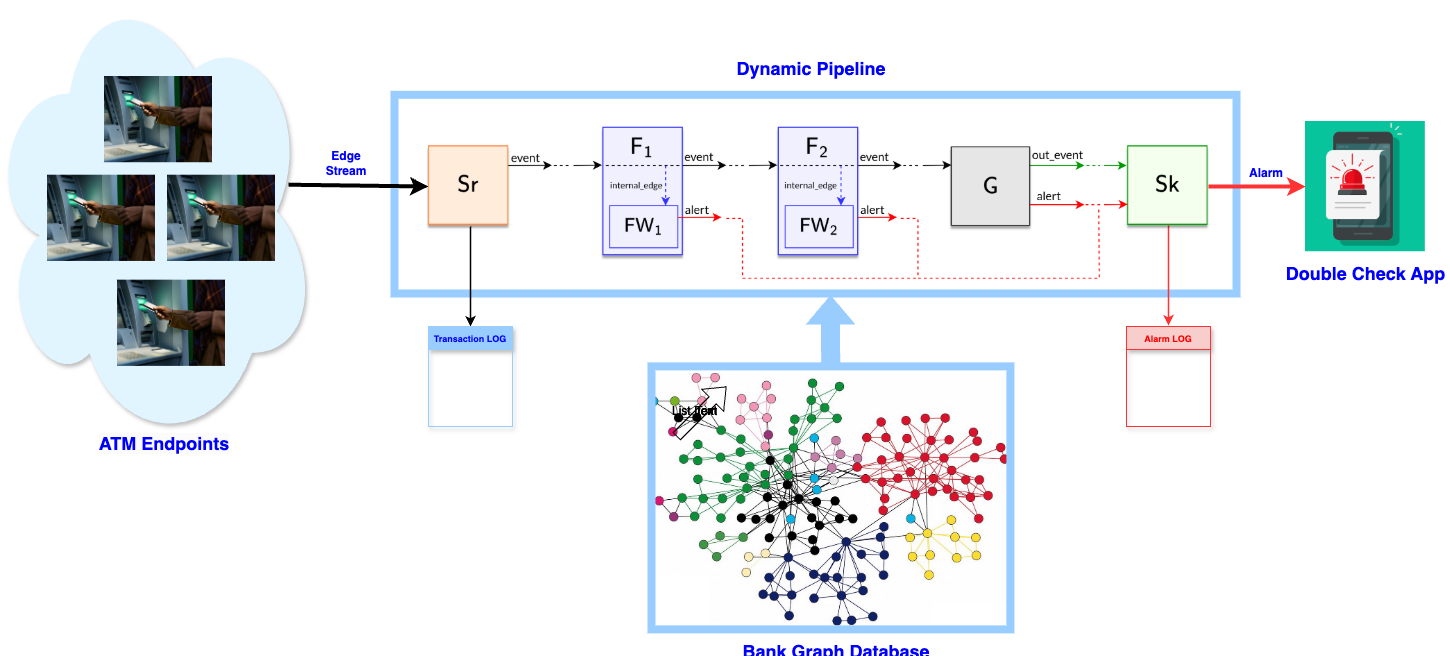
\includegraphics[scale = 0.32]{images/architectureCQE.png}
         \caption{Abstraction of the Continuous Query Engine for detecting anomalous 
         ATM transactions based on the dynamic pipeline computational model. 
         In this abstract architecture of the Continuous Query  all its components as well as its expected usage are shown. }
         \label{fig:architecture-usage}
\end{figure}
%
%Still we are working on the design and implementation of this model. 
As we said, we propose a solution that follows the Dynamic Computational Approach \cite{DP-pasarella2024computational}. Briefly speaking, in this approach, \emph{stages} are processes that execute tasks concurrently/in-parallel. The multiset underlying the input data stream is partitioned \cite{bender1974partitions} and distributed along filters according to a grouping relationship, usually based on filters' parameters. Each filter applies the same function to its block of data (stored as its state). Accordingly, the  $\mathsf{DP_{ATM}}$ algorithm is specified as follows: During a pre-defined time interval window, when an \textsf{interaction} $\mathsf{e}$ (together its properties' values)  arrives to the $\mathsf{DP_{ATM}}$, the stage $\mathsf{S_r}$ register it into a standard transactional log file. Then, $\mathsf{S_r}$ passes $\mathsf{e}$ to the next stage. If there exists a filter parameterized with the value of the property \textsf{number} of the Card vertex that is incident to  $\mathsf{e}$, this filter keeps $\mathsf{e}$ in its state. In this way, filters' states store  subgraphs induced by the edges in the volatile subgraph. Notice that these sets of edges in each filter correspond to blocks of the (multiset) input data stream.  Otherwise, the filter passes $\mathsf{e}$ to the next stage. The task/function of each filter is to decide if there is a match with (some of) the continuous query pattern(s) evaluated by the engine $\mathsf{DP_{ATM}}$ by means of the graph that it stores and the information retrieved from the stable PG to identify patterns and solve constraints. This is, indeed, the way to evaluate continuous queries. In case of matching a pattern, filters emit an alert reporting the finding. Hence, answers are the detected anomalies and they are emitted as they are obtained in filters. When answers arrive to $\mathsf{S_k}$, this stage  post-processes  and output  them. In addition, $\mathsf{S_k}$ maintains an answer log file. The fact that an \textsf{interaction} arrives to $\mathsf{G}$ means that there were not previous interactions having the same value of Card property \textsf{number} and thus, a new filter parameterized with this new value is spawned. When the time interval window is over, the $\mathsf{DP_{ATM}}$ is, in some sense, reset according to the given window policy. Note that the window policy must take into account stored data that might be valid in between two windows and handle the transition properly.
%
\subsection{Defining Anomalous Patterns of Transactions}\label{sub:anomalouspatterns}
It is not trivial to establish what is and in which circumstances a transaction can be considered anomalous. Based on a work that have addressed this characterization \cite{magdalena2021artificial} we intend to find a proper characterization and then define the graph patterns associated to these anomalies. The exact topology of an anomaly will depend on its own nature. Figure \ref{fig:constinuousPGb} depicts an example characterizing a possible card cloning, among many other possibilities. For instance, using a (stolen) card many times over a period of time at different ATMs to withdraw small amounts. In this latter case, there will arrive to the evolving PG many volatile (interaction) edges having the same card vertex and different ATM vertices. There could also be patterns related with frequent/very high expenses; transactions  located in an ATM out of the threshold distance of the usual/registered address of the card holder and so on.
Moreover, definition of patterns can be beyond ATM transactions by considering Point-Of-Sale (POS) or online card transactions.
%
\iffalse
\subsubsection*{Fraud Patterns Definition}

It is not trivial to establish what is and in which circumstances an ATM transaction can be considered anomalous. Based on a work that have addressed this characterization \cite{FP-magdalena2021artificial} we intend to find a proper characterization and then define the graph patterns associated to these anomalies. The exact topology of an anomaly will depend on its own nature. Moreover, definition of patterns can be beyond ATM transactions by considering online card transactions. In what follows, we propose a characterization of some possible anomalous patterns of ATM transactions and the definition of their associated PG graph patterns. 
\fi
%
\begin{enumerate}
\renewcommand{\labelenumi}{\Roman{enumi}.} % Roman numerals for the list
    \item Card cloning characterization
    \item Lost-and-stolen card characterization
    %\item Anomalous amount of withdrawals in a time period
    \item Other possible fraud scenarios
\end{enumerate}


\paragraph{I - Card Cloning Characterization\\\\}

\emph{Card cloning} can be defined as "a kind of fraud in which information on a card used for a transaction is covertly and illegally duplicated. 
Basically, it’s a process thieves use to copy the information on a transaction card without stealing the physical card itself. 
This information is then copied onto a new or reformatted card, allowing criminals to use it to make fraudulent purchases or gain unauthorized access to a person’s accounts" \cite{FP-unit21_card_cloning}.\\

There are many possible ways to detect a card cloning scenario, among others, the analysis of the customer's transaction data to construct typical transaction behaviors so to be able to detect uncommon transaction behaviors. However, in our work we propose an alternative possible method based on a PG graph pattern detection.\\

The method consists on detecting abnormal card-ATM activity of the same card at different ATMs taking place within an unfeasible time distance difference. That is, when a transaction is made at an ATM, and after that, another transaction is initiated with the same card at a different ATM, such that the distance between the two is impossible to be covered within the time between the transactions.
The detection of this anomalous scenario is represented on the PG graph pattern of Figure \ref{img:graphPattern-1}. 

\begin{figure}[H]
  \centering
  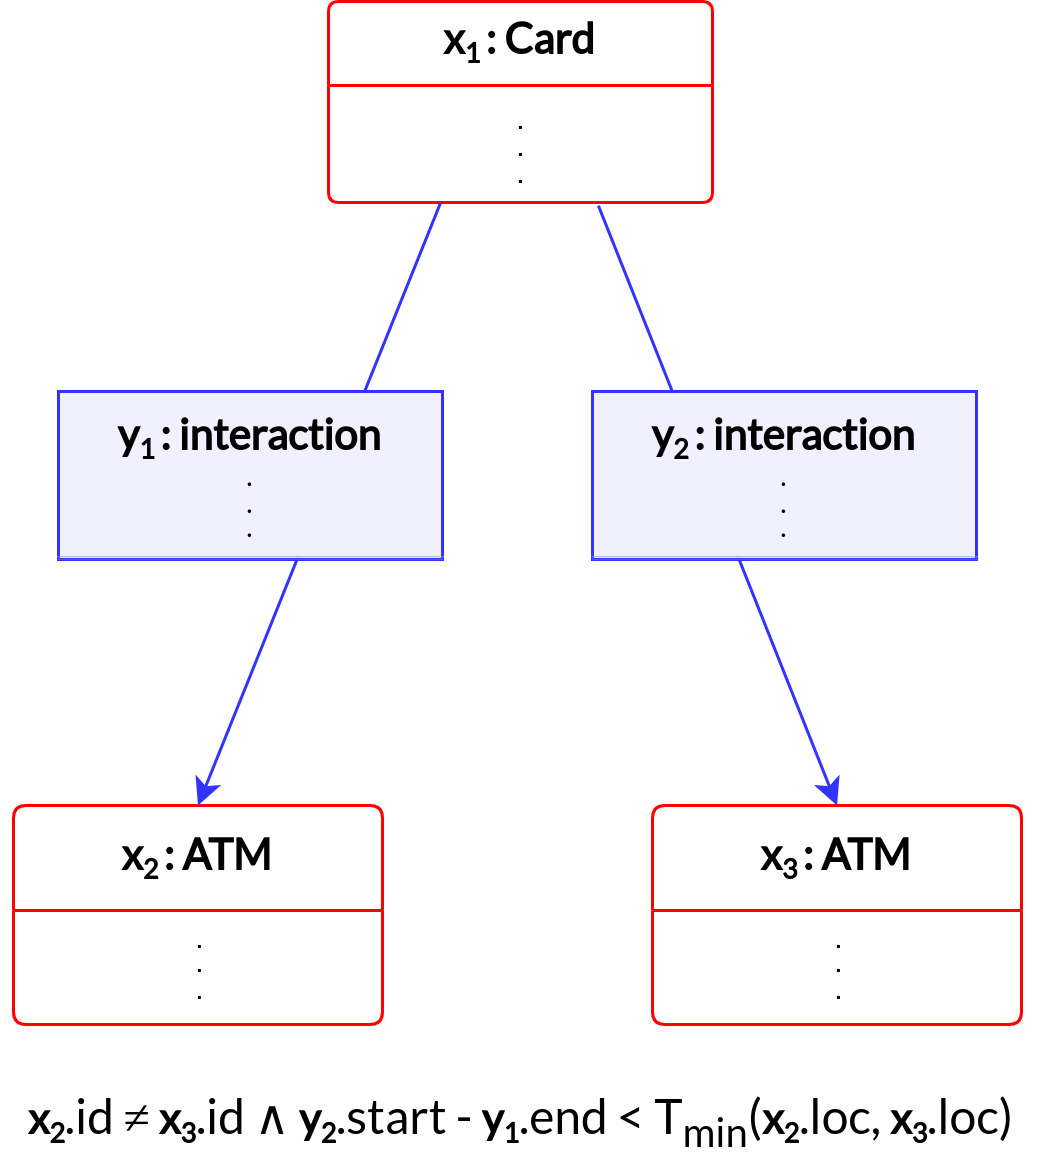
\includegraphics[scale = 0.8]{images/2-QueryModel/graphPattern-1.png}
  \caption{Property graph pattern - Card cloning characterization}
  \label{img:graphPattern-1}
\end{figure}

The pattern consists on a \texttt{Card} entity $x_1$, having two \texttt{interaction} relations $y_1$ and $y_2$ with two different \texttt{ATMs} $x_2$ and $x_3$, respectively, such that the time difference between the ending time of the first \texttt{interaction} $y_1.\textit{end}$ and the starting time of the second \texttt{interaction} $y_2.\textit{start}$, is not sufficient to cover the minimum time needed to travel from the first to the second \texttt{ATM} location $T_{min}(x_2.\textit{location}, x_3.\textit{location})$. As a whole:

$$
\small
x2.id \ne x3.id \ \land \ y_2.\textit{start} - y_1.\textit{end} < T_{min}(x_2.\textit{location}, x_3.\textit{location})
$$

where $x_2.\textit{location}$ represents the location coordinates pair of the $x_2$ ATM: $x_2.location = (x_2.loc\_latitude, x_2.loc\_longitude)$. Same for the \texttt{ATM} $x_3$.\\

An example of this kind of anomalous card-ATM interaction, could be one as represented on Figure \ref{img:graphPattern-1-Example}, in which an ATM interaction with a certain card is finished at time 22:14 in Barcelona, and then another interaction with that same card starts at time 22:56 of that same day in Madrid. Clearly this should be reported as this kind of anomalous scenario since it is impossible, for the time being, to cover the distance between these two cities in that time interval.

\begin{figure}[H]
  \centering
  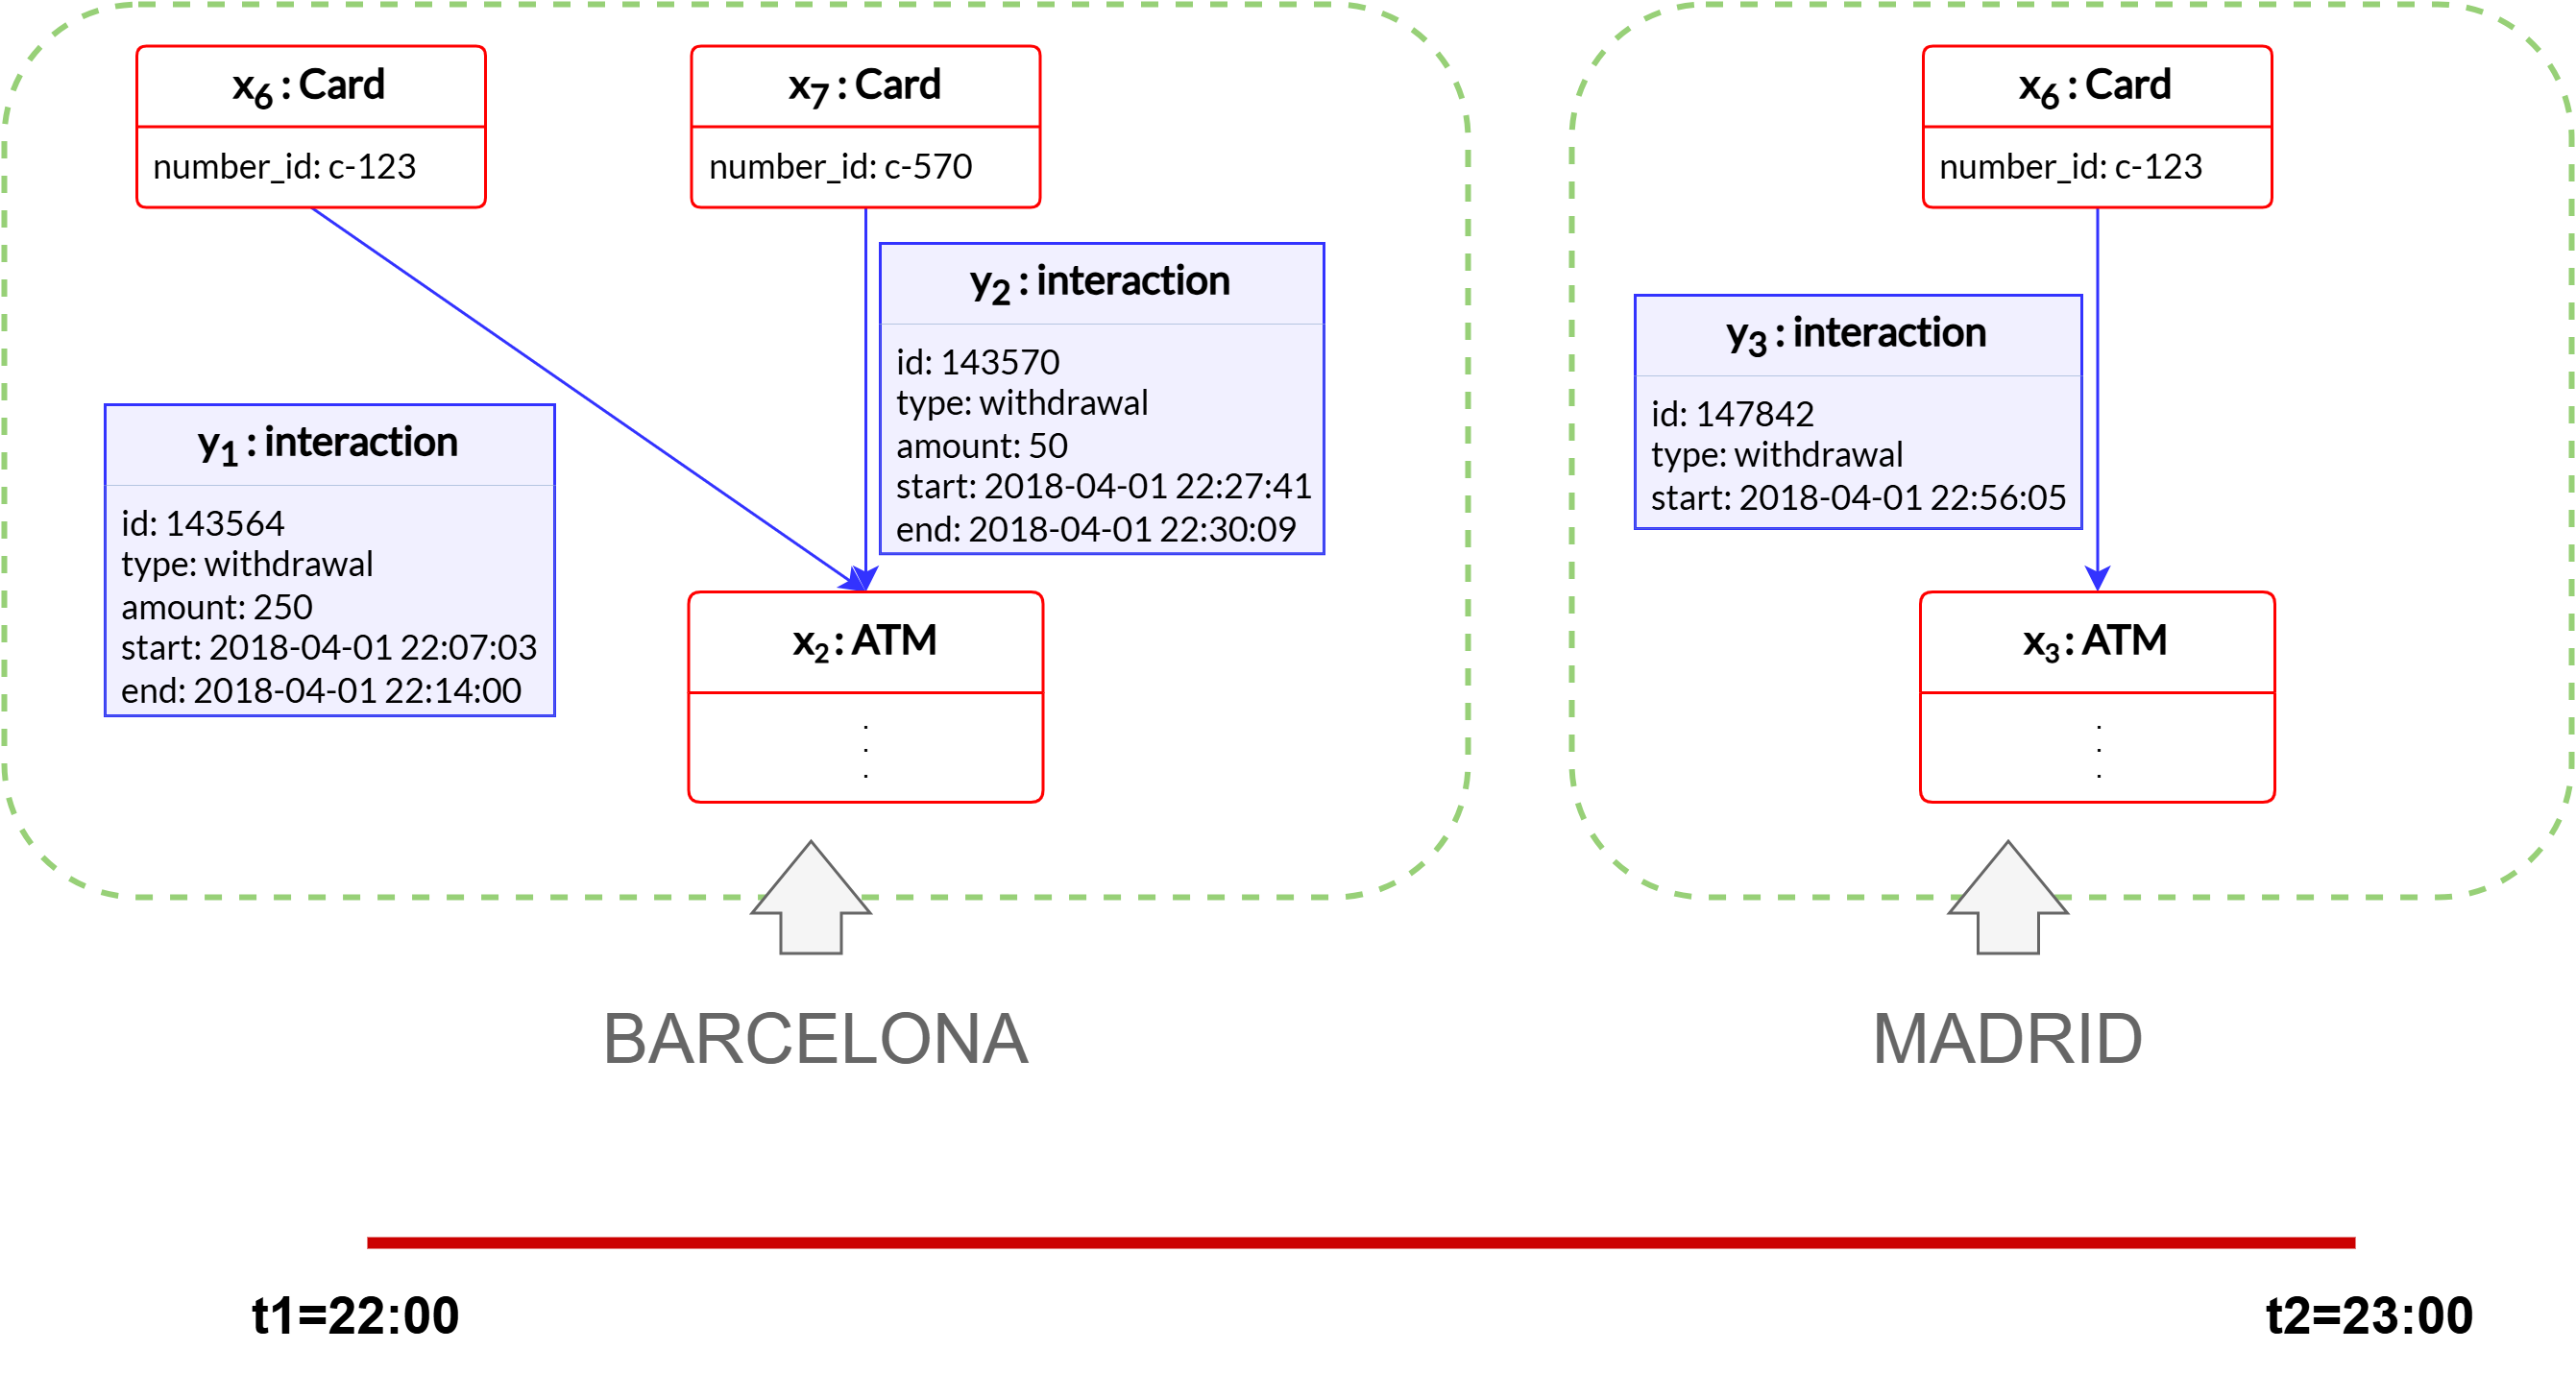
\includegraphics[scale = 0.7]{images/2-QueryModel/FP1-Example.png}
  \caption{Card cloning characterization - an example}
  \label{img:graphPattern-1-Example}
\end{figure}

\paragraph{II - Lost-and-Stolen Card Characterization\\\\}

"Lost-and-stolen card is the fraud scenario produced when a card is physically stolen or is lost, and is then used by a criminal, posing as you, to obtain goods and services" \cite{FP-lost-and-stolen-americanexpress2025}.\\

A possible way that we propose to detect this kind of fraud scenario is through the tracking of a typical behavior that it is produced when the card is used by the criminal. That is, when obtained, the fraudster tries to do as many as possible money withdrawals in different ATMs before the owner of the card become aware of the loss of the card and asks the bank to freeze it. The detection of this kind of fraud scenario is modeled with a PG graph pattern as the one represented in Figure \ref{img:graphPattern-2}.

\begin{figure}[H]
  \centering
  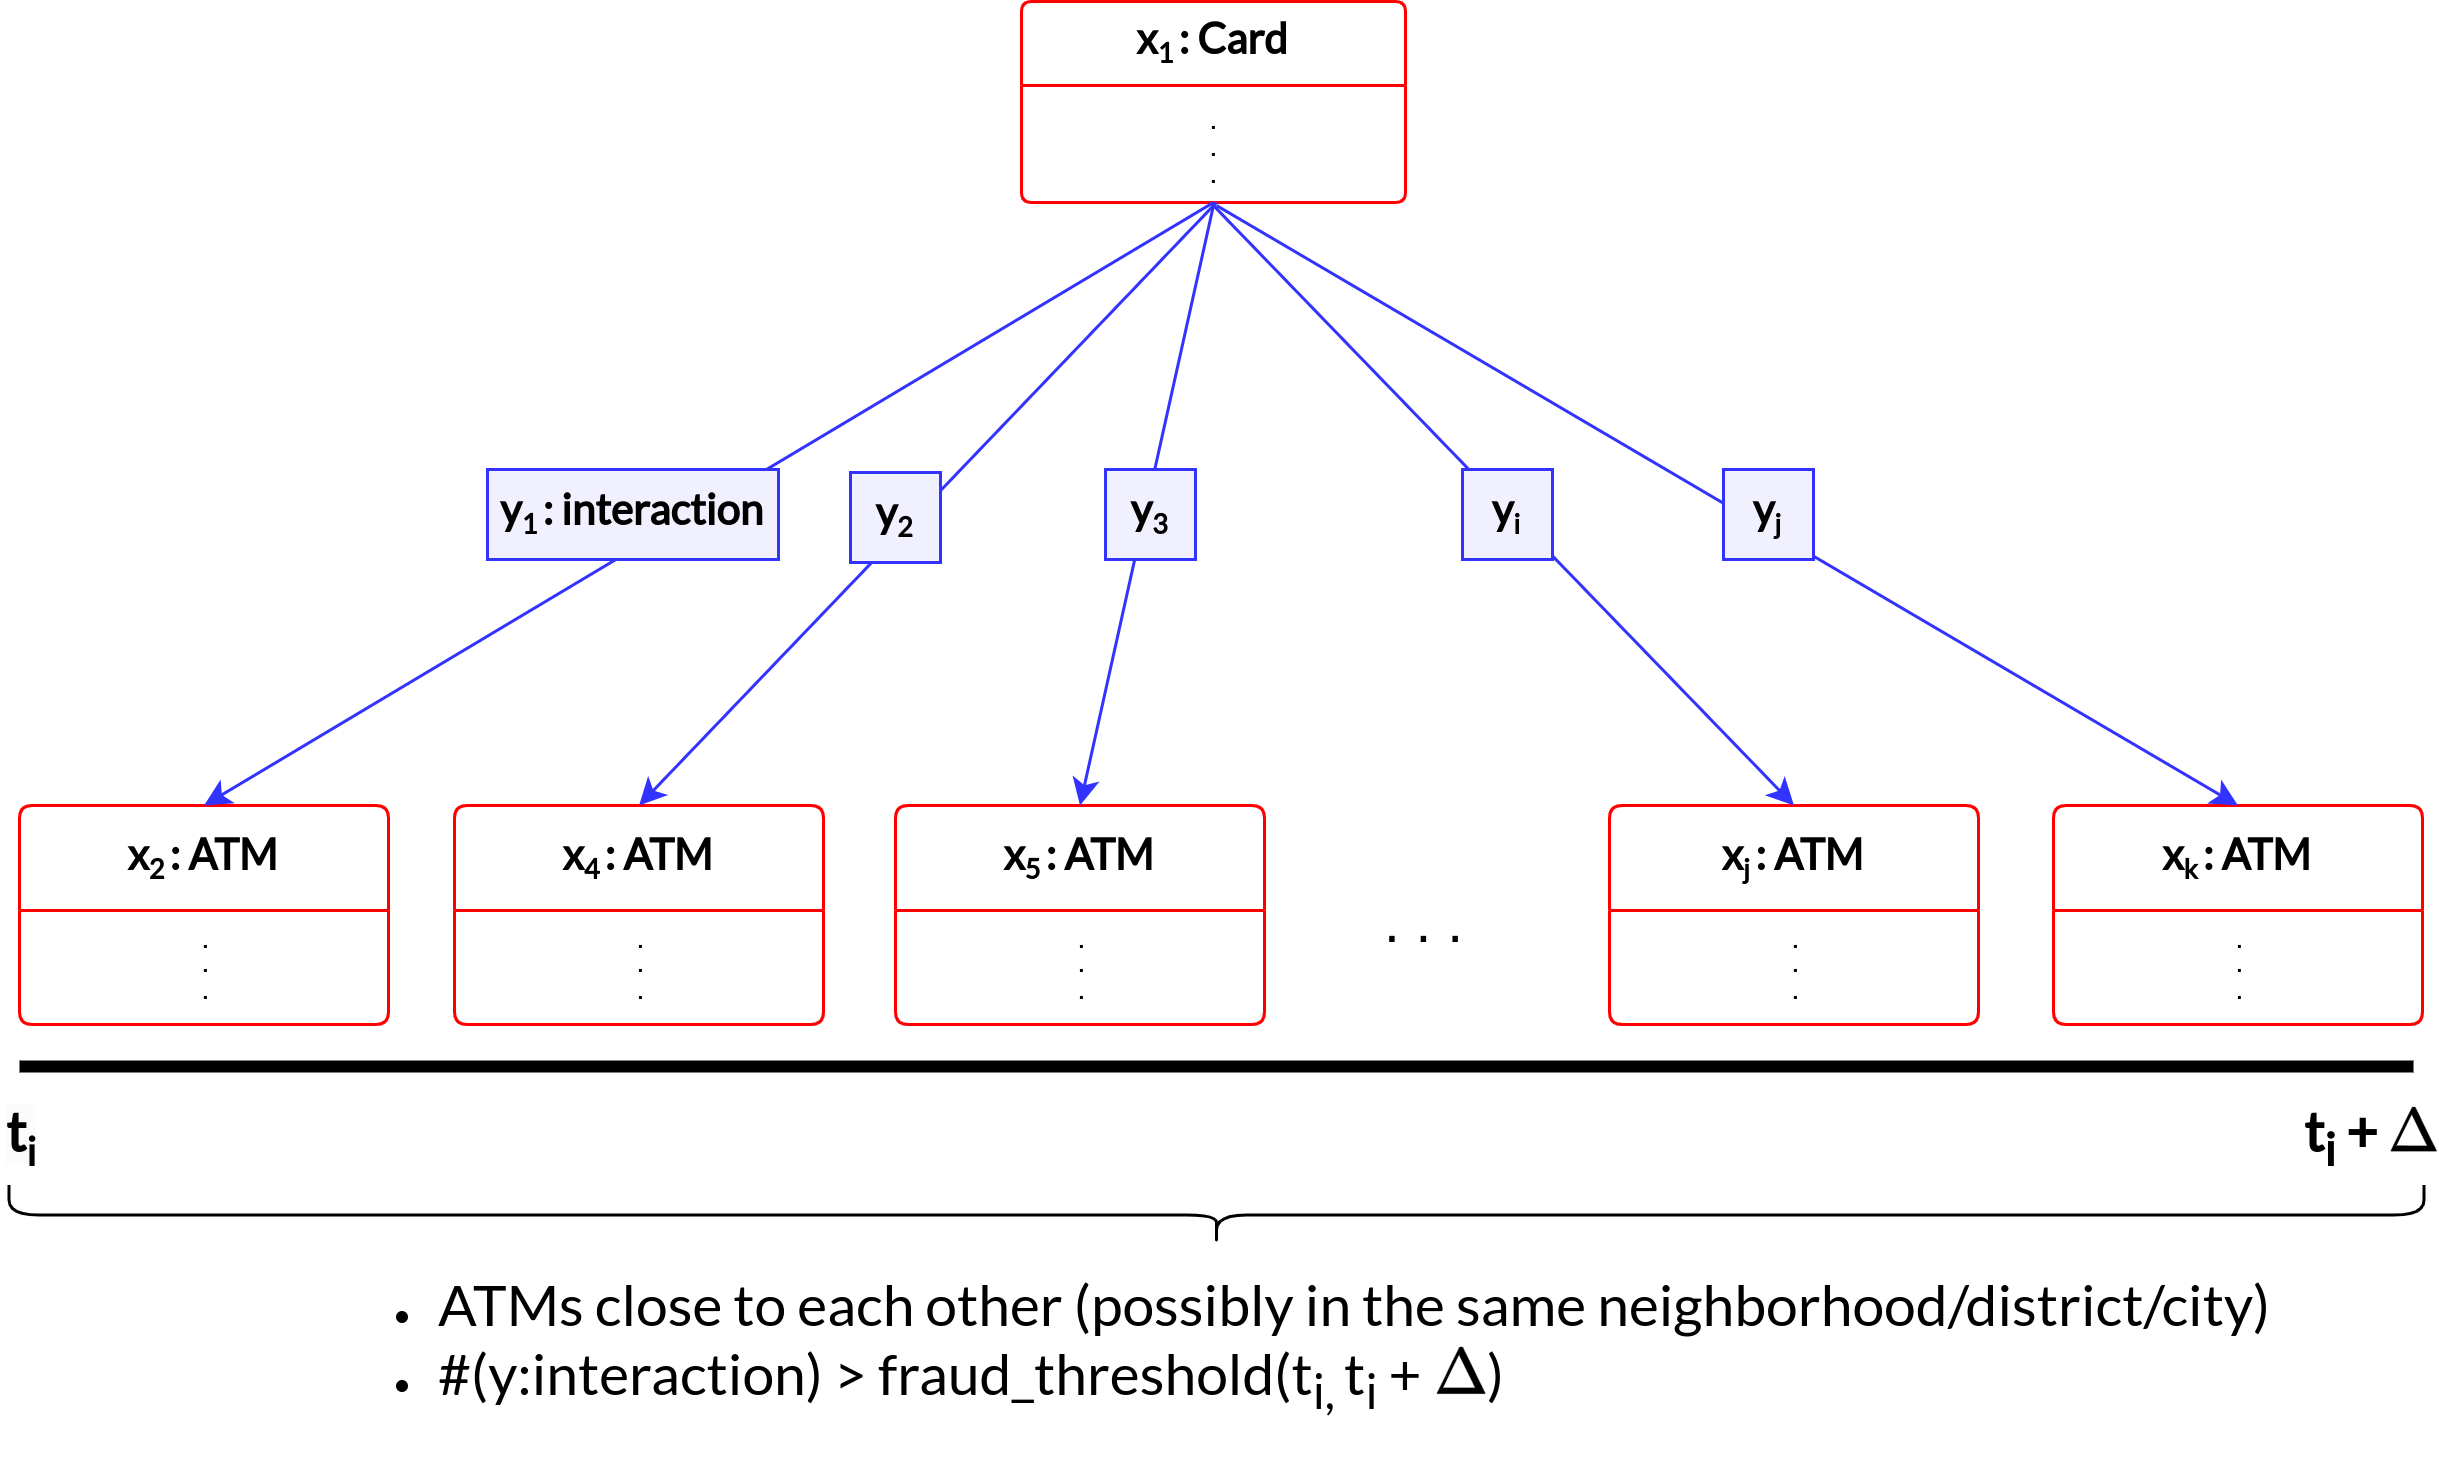
\includegraphics[scale = 0.7]{images/2-QueryModel/graphPattern-2.png}
  \caption{Property graph pattern - Lost-and-stolen card characterization. The interactions $y_1,...,y_j$ depicted are of the \emph{type} withdrawal}
  \label{img:graphPattern-2}
\end{figure}

On it we define a \texttt{Card} entity $x_1$ having a number $k$ of \texttt{interactions} $y$ at different \texttt{ATMs} $x_2 ... x_k$ within a time interval $[t_i, t_i + \Delta]$, where $t_i = y_1.\textit{start}$ and $t_i + \Delta = y_j.\textit{start}$, such that $k$ is considered to be an usual high number of withdrawals for that time interval. A reference for the usual number of withdrawals on a certain time interval for a specific cardholder can be obtained from the gathered cardholder behavior (in our case represented as the \emph{withdrawal\_day} \texttt{Card} entity property of our defined data model).
Another indicator of this scenario to be considered could also be the \emph{amount} value of the withdrawal operations performed, which, in these scenarios, is normally a low value to prevent that the card owner realises.

\paragraph{III - Other Possible Fraud Scenarios\\\\}

Some other anomalous scenarios for which more graph patterns could be defined are:
\begin{itemize}
    \item \textbf{Anomalous location usage}: When a transaction is made in a location out of the threshold distance of the usual/registered address of the cardholder.
    \item \textbf{Anomalous number of operations}: Related with the II pattern characterized, we could also define a graph pattern related with a higher than average number of operations of any kind (withdrawal, inquiry, transfer or deposit) for a cardholder in a certain time interval.
    \item \textbf{Anomalous high expenses:} Similar to the II pattern, but in this case, not considering only the number of the withdrawal operations performed on a certain time interval, but the amount of the withdrawal operations on a certain time interval. This could indicate an anomalous behavior of the cardholder, withdrawing an amount of money way higher for a considered time interval.
\end{itemize}

%


\section{Data Model}

%\textcolor{red}{$\rightarrow$ TODO: Explanation of the PG data model chosen - details, reason why...}

\begin{comment}
\textcolor{gray}{Nowadays data are in motion, change continuously and are -possibly- unbounded implying data
sources that are also constantly evolving. From the data persistence point of view this reality breaks the
usual paradigm of having dynamic but stable data sources. This, together with the increasing number
applications based on data streams for taking critical decisions in real time, raises the need for re-thinking
both the data and the query models to fit these new requirements. Therefore, under these circumstances,
it seems reasonable that a suitable data model is a continuously evolving data graph.\\
...
Regarding the data model, the new nature of data requires a de facto new database paradigm
-continuously evolving databases- where data can be both stable and volatile. Even though
evolving databases can be implemented according to any approach, graph databases seem
especially well suited here [1, 2]. Indeed, the natural way to process evolving graphs as streams
of edges gives insights on how to proceed in order to maintain dynamic graph databases. Hence,
we consider that a suitable data model is a continuously evolving data graph, a graph having
persistent (stable) as well as non persistent (volatile) relations. Stable relations correspond
to edges occurring in standard graph databases while volatile relations are edges arriving indata streams during a set time interval. Once this time interval is over, the relations are not
longer valid so that there is no need to store them in the (stable) graph database. However,
when required -as for further legal or auditing purposes- timestamped occurrences of volatile
relations can be kept in a log file. Volatile relations induce subgraphs that exist only while the
relations are still valid. Without loss of generality, in this work we consider property graphs
(PG) [3, 4] as the basic reference data model. As an example, Figure 1a depicts part of a schema
of a PG database where stable relations correspond to the data that a bank typically gathers
on its issued cards, ATMs (Automated Teller Machines) network, etc. Volatile relations model
the interaction between cards and ATM entities}
\end{comment}

The property graph data model consists of two sub property graphs: a stable and a volatile property graph. On the one hand, the stable is composed of the static part of the data that a bank typically gathers such as information about its clients, cards, ATMs (Automated Teller Machines). 
On the other hand, the volatile property graph models the transaction operations, which defines the most frequent and reiterative kind of interaction between entities of the data model.\\
The main difference and the main reason for this separation is the semantics with which we intentionally define each of the subgraphs: the stable will be understood like a fixed static bank database, whereas the volatile will be understood as the data model to define the transactions, as continuous interactions between the entities of the model, which will not be permanently saved, but instead, only for a certain window of time under the mission of detecting anomalous bank operations. Note that we will only model the transaction interaction in the volatile subgraph, only letting them occur here.
This separation will allow us to have a really simple and light property graph schema single-centered on the transactions with the minimal needed information (mostly identifiers of the entities a transaction links) and another, the stable, acting as a traditional bank database schema, from which to obtain the information details of the entities.

\subsection{Property Graph Design}

In what follows we provide the description of the design of our proposed
Property Graph data model, divided into the stable and volatile property
graphs.

\subsubsection{Stable Property Graph}

Due to the confidential and private nature of bank data, it was
impossible to find a real bank dataset nor a real bank data model. Therefore, we devoloped our own proposal of a bank database model.
We propose a simplified data model where the defined entities, relations and properties are reduced to the essential ones.
Although it is obvious that a real bank data model is way more complex than the one we propose, we believe that ours is relevant and representative enough and therefore sufficient for the purpose of our work. 

\begin{figure}[H]
    \centering
    \includegraphics[scale = 0.7]{sections/1-DataModel/images/PG-stable-edit-cardinal.png}
    \caption{Initial bank stable property graph model}
    \label{img:initial-pg-stable}
\end{figure}

% TODO: Cómo pongo que se entienda bien el 1er modelo y su correspondiente transformación al segundo y definitivo: explicando también en el medio las entidades, relaciones y atributos y su elección.
A first model proposal was the one shown in Figure \ref{img:initial-pg-stable}.
Basically, the idea of this first model attempt was to capture the data that a bank system database typically gathers.
It contains four entities: Bank, ATM, Client and Card with their respective properties, and the corresponding relationships between them.
The relations are: a directed relationship from Client to Card \texttt{owns} representing that a client can own multiple credit cards and that a card is owned by a unique client, then a bidirectional relation \texttt{has\_client} between Client and Bank; representing bank accounts of the clients in the bank. The relation between Card and Bank to represent that a card is \texttt{issued\_by} the bank, and that the bank can have multiple cards issued. Finally, the relations \texttt{belongs\_to} and \texttt{interbank} between the ATM and Bank entities, representing the two different kinds of ATMs depending on their relation with the bank; those ATMs owned and operated by the bank and those that, while not owned by the bank, are still accesible for the bank customers to perform transactions.

\begin{figure}[H]
    \centering
    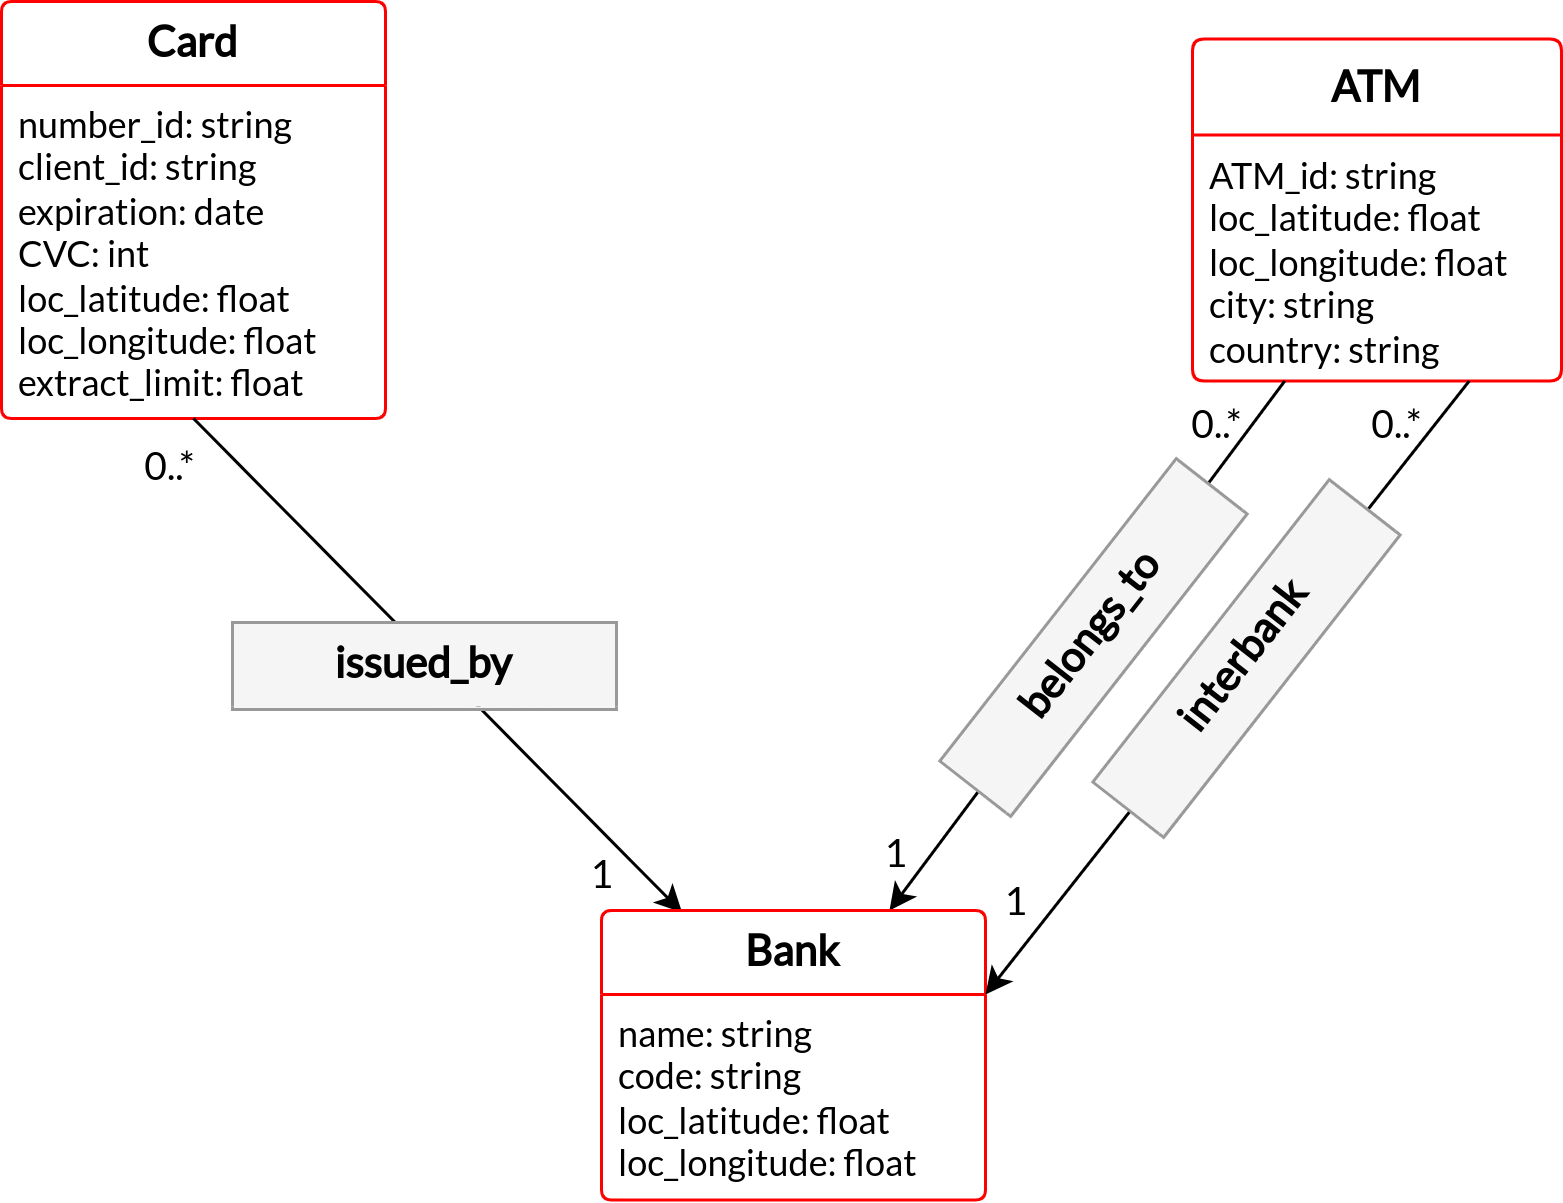
\includegraphics[scale = 0.7]{sections/1-DataModel/images/PG-stable-1-edit-cardinal.png}
    \caption{Definitive stable property graph model}
    \label{img:pg-stable-def}
\end{figure}

However, the final version of the model (see Figure \ref{img:pg-stable-def}) was simplified to reduce it to the minimal needed entities. In particular, we decided to remove the Client entity and to merge it inside the Card entity. This reduction allows to simplify the stable property graph to only three entities. 
For this, all the Client attributes were included in the Card entity. In the initial schema the Client entity was defined with three attributes: the identifier of the client and the GPS coordinates representing the usual residence of the client. This change is done while preserving the restriction of a Card belonging to a unique client the same way it was previously done with the relation between Card and Client \texttt{owns} in the initial schema, which now is therefore removed. \\
% Account relation removed
Another derived consequence of this simplification is the removal of the other relation that the Client entity had with other entities: the \texttt{has\_client} relation between Client and Bank, which was originally made with the intention of representing the bank accounts between clients and banks. Maintaining a bank account would imply having to consistently update the bank account state after each transaction of a client, complicating the model. Nevertheless, we elimintate the bank account relation, since its removal is considered negligible and at the same time helpful for the simplification of the model needed for the purposes of our work. However, for the sake of completeness the attribute \textit{extract\_limit} is introduced in the Card entity, representing a money amount limit a person can extract, which will be related with the amount of money a person owns. This will allow the detection of anomalies related with frequent or very high expenses.


\begin{comment}
The final entities and their selected attributes are described in what follows:

\paragraph{Entities\\}

\paragraph{Bank}

\begin{itemize}
\item[-] name: Bank name.
\item[-] code: Bank identifier code.
\item[-] loc\_latitude: Bank headquarters GPS-location latitude.
\item[-] loc\_longitude: Bank headquarters GPS-location longitude.
\end{itemize} 

\begin{figure}[H]
    \centering
    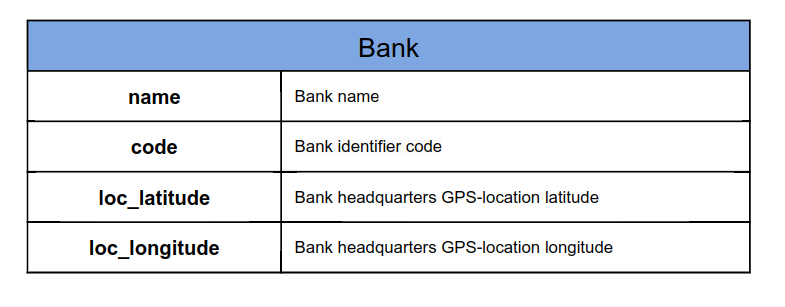
\includegraphics[scale = 0.4]{images/bank.png}
    \caption{Bank entity attributes}
    \label{img:pg-bank}
\end{figure}

\paragraph{ATM}

\begin{itemize}
\item[-] ATM\_id: Unique identifier of the ATM.
\item[-] loc\_latitude: GPS-location latitude where the ATM is located.
\item[-] loc\_longitude: GPS-location longitude where the ATM is located.
\item[-] city: City in which the ATM is located.
\item[-] country: Country in which the ATM is located.
\end{itemize}

\begin{figure}[H]
    \centering
    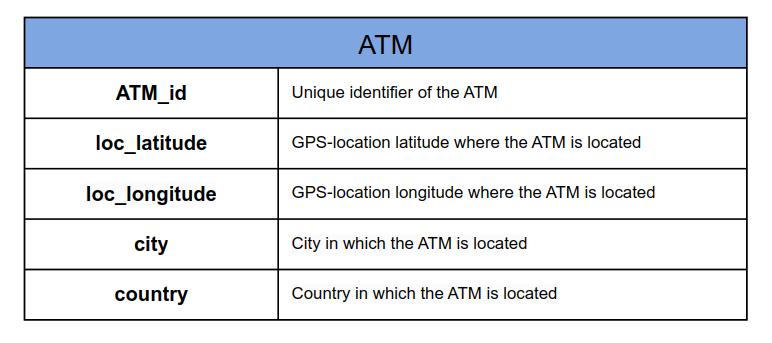
\includegraphics[scale = 0.4]{images/atm.png}
    \caption{ATM entity attributes}
    \label{img:pg-atm}
\end{figure}


\paragraph{Card}

\begin{itemize}
\item[-] number\_id: Unique identifier of the card.
\item[-] client\_id: Unique identifier of the client.
\item[-] expiration: Validity expiration date of the card.
\item[-] CVC: Card Verification Code.
\item[-] extract\_limit: Limit amount of money extraction associated with the card.
\item[-] loc\_latitude: Client address GPS-location latitude.
\item[-] loc\_longitude: Client address GPS-location longitude.
\end{itemize}

\begin{figure}[H]
    \centering
    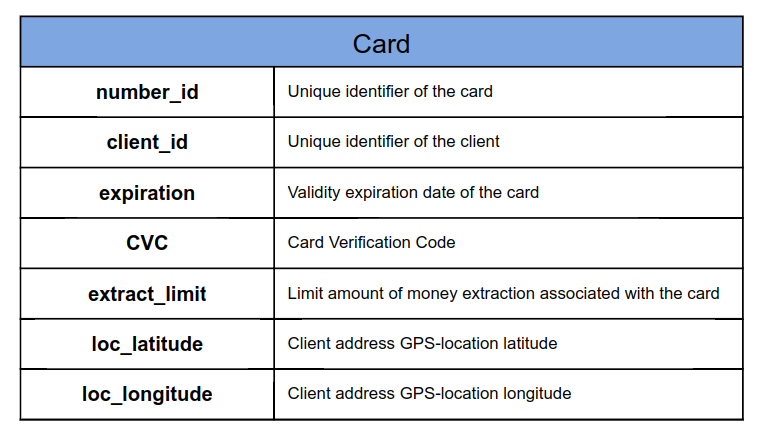
\includegraphics[scale = 0.4]{images/card.png}
    \caption{Card entity attributes}
    \label{img:pg-card}
\end{figure}

Note that for both the ATM and the Card entities we have the GPS coordinates information. In the first case referring to the geolocation of each specific ATM and in the last case referring to each specific client address geolocation. This will be useful to be able to detect transaction frauds related to geolocation distances.

Note that the client is completely anonymized in the system (no name, surname, age, or any other confidential details) by using only a client\_id. For the present purpose it is enough to uniquely identify each client.

% Relations -> and its attributes
\paragraph{Relations}
There are only two relations in the final stable subgraph, that is, the ones that are left after the deletion of the Client entity from the first version of the stable subgraph; the relation "issued\_by" between the Card and the Bank entities and the "belongs\_to" between ATM and Bank entities. For the moment they do not have any attribute, however they could potentially be added in the case this was needed.

\end{comment}

\subsubsection{Volatile property graph}
\textcolor{red}{$\rightarrow$ TODO: describe}

\begin{comment}
It contains the minimal needed information to be able to recognize the anomaly fraud patterns we want to identify.
This subgraph describes the most volatile part of our model, meaning the transactions between the client's cards and the ATMs. The idea is to have a data model to define the transactions, as continuous temporal interactions between the Card and ATM entities, restricting these kind of relations to the volatile subgraph.
The idea is to have a really simple and light property graph schema single-centered on the transactions. For that the Card and ATM entities will be simplified to the last bullet, containing only the identifier of the both entities that each transaction relation matches. These identifiers will be enough to be able to recover, if needed, the whole information about the specific Card or ATM entity in the stable subgraph.

\begin{figure}[H]
    \centering
    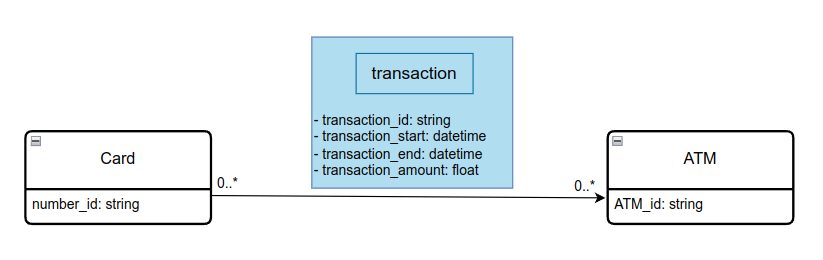
\includegraphics[scale = 0.45]{images/diagPG-volatile.png}
    \caption{Volatile property graph model}
    \label{img:pg-stable}
\end{figure}

Following this idea of volatile subgraph, the Card and ATM entities and transaction relations of it will not be permanently saved, but instead, only for a certain window of time under the mission of detecting anomalous bank operations. 

The transaction relation will include some attributes that will be essential for the detection of the fraud patterns, in particular:

\begin{itemize}
\item[-] transaction\_id: Unique identifier for each transaction in the database.
\item[-] transaction\_start: Datetime when the transaction started. Format: DD/MM/YYYY HH:MM (ex. 1/1/2022 4:50).
\item[-] transaction\_end: Datetime when the transaction was completed. Format: DD/MM/YYYY HH:MM (ex. 1/1/2022 4:54).
\item[-] transaction\_amount: Amount of money involved in the transaction.
\end{itemize}

\begin{figure}[H]
    \centering
    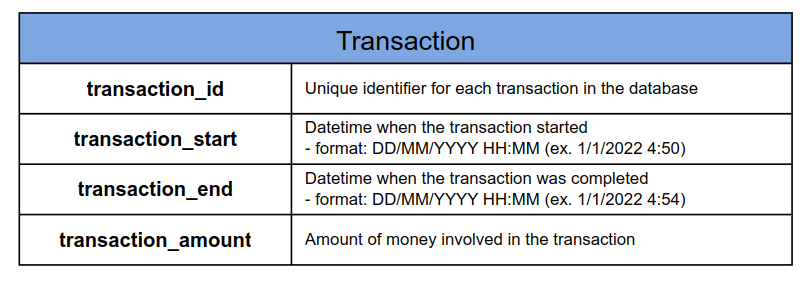
\includegraphics[scale = 0.40]{images/transaction.png}
    \caption{Transaction relation attributes}
    \label{img:pg-stable}
\end{figure}
\end{comment}
\textcolor{green}{\rule{\linewidth}{0.4mm}}
\subsection{Synthetic dataset creation}

As mentioned, given the confidential and private nature of bank data, it was not possible to find
any real bank datasets. In this regard, a synthetic property
graph bank dataset was built based on the \emph{Wisabi Bank Dataset}\footnote{\href{https://www.kaggle.com/datasets/obinnaiheanachor/wisabi-bank-dataset}{Wisabi bank dataset on kaggle}}. It is a fictional banking dataset that was made publicly available in
the Kaggle platform.

This synthetic bank dataset was considered of interest as a base for the synthetic bank
database that we wanted to develop. The interest to use this bank dataset as a base was mainly because of its size: it contains 8819 different customers, 50 different ATM locations and 2143838 transactions records of the different customers during a full year (2022). Additionally, it provides good heterogenity on the different kind of transactions: withdrawals, deposits, balance inquiries and transfers.

The main uses of this bank dataset are the obtention of a geographical distribution for
the locations of our generated ATMs and the construction of a card/client \emph{behavior},
for which the data of the \emph{Wisabi Bank Dataset} will be used.

\paragraph{Details of the \emph{Wisabi Bank Dataset}}
The \emph{Wisabi Bank Dataset} consists on ten CSV tables. Five of them are of transaction records of five different states of Nigeria (Federal Capital Territory, Lagos, Kano, Enugu and Rivers State) that refers to transactions of cardholders in ATMs. In particular they contain 2143838 transactions records done during the year 2022, of which 350251 are in Enugu, 159652 in Federal Capital Territory, 458764 in Kano, 755073 in Lagos and 420098 in Rivers. Then, the rest of the tables are: a customers table (`customers\_lookup`) where the data
of 8819 different cardholders is gathered, an ATM table (`atm\_location lookup`) with
information of each of the 50 different locations of the ATMs, and then three remaining
tables as complement of the previous ones (`calendar lookup`, `hour lookup` and 
`transaction\_type lookup`) 
(\href{https://app.diagrams.net/#G1eAn47YR7-zPNE5KgStkA6_IJcxZRYgX8#%7B%22pageId%22%3A%22R2lEEEUBdFMjLlhIrx00%22%7D}{tables summary}).

In what follows we give the details on the generation of the instances of our static database
entities.
For simplicity and to do it in a more stepwise manner, we are going to first create all the CSV data tablesfor the nodes and for the relations in the corresponding format and then we will populate the Neo4j GDB with them.

$\rightarrow$ To do the generation of a stable bank database use the Python program \texttt{bankDataGenerator.py}, in which you will have to enter the bank properties' values, 
as well as the parameters on the number of the bank ATMs and Cards: \texttt{n} and \texttt{m}, respectively.

\subsubsection*{Bank}

Since a unique bank instance is considered, the values of the properties of the bank node are 
manually assigned, leaving them completely customisable. Bank node type properties consist
on the bank \emph{name}, its identifier \emph{code} and the location
of the bank headquarters, expressed in terms of \emph{latitude} and \emph{longitude}
coordinates, as seen in Table \ref{table:bank-node-properties}.
For the bank, we will generate \texttt{n} ATM and \texttt{m} Card entities. Note that 
apart from the generation of the ATM and Card node types we will also need to generate 
the relationships between the ATM and Bank entities (\texttt{belongs\_to} and \texttt{interbank}) 
and the Card and Bank entities (\texttt{issued\_by}).

\begin{table}[H]
    \centering
      \begin{tabular}{|l|l|}
      \hline
      \textbf{Name}        & \textbf{Description and value}                                      \\ \hline
      \texttt{name}         & Bank name                                                 \\ \hline
      \texttt{code}         & Bank identifier code                                      \\ \hline
      \texttt{loc\_latitude}  & Bank headquarters GPS-location latitude                   \\ \hline
      \texttt{loc\_longitude} & Bank headquarters GPS-location longitude                  \\ \hline
      \end{tabular}
    \caption{Bank node properties}
    \label{table:bank-node-properties}
\end{table}

\subsubsection*{ATM}

\begin{table}[H]
    \centering
    \begin{tabular}{|l|l|}
    \hline
    \textbf{Property}        & \textbf{Description}                                      \\ \hline
    \texttt{ATM\_id}      & ATM unique identifier                             \\ \hline
    \texttt{loc\_latitude}  & ATM GPS-location latitude           \\ \hline
    \texttt{loc\_longitude} & ATM GPS-location longitude          \\ \hline
    \texttt{city}         & ATM city location                         \\ \hline
    \texttt{country}      & ATM country location                       \\ \hline
    \end{tabular}
    \caption{ATM node properties}
    \label{table:atm-node-properties}
\end{table}

The bank operates \texttt{n} ATMs, categorized in:

\begin{itemize}
  \item Internal ATMs: ATMs owned and operated by the bank. They are fully integrated within the
  bank's network. Modeled with the \texttt{belongs\_to} relation.
  \item External ATMs: These ATMs, while not owned by the bank, are still accessible for the bank
  customers to perform transactions.  Modeled with the \texttt{interbank}  relation. 
\end{itemize}

Both types of ATMs are considered to be of the same type of ATM node. Their difference
is modeled as their relation with the bank instance: \texttt{belongs\_to} for the internal ATMs and \texttt{interbank} for the external ATMs, having:
$$\texttt{n = n\_internal + n\_external}$$

where \texttt{n\_internal} is the number of internal ATMs owned by the bank and \texttt{n\_external}
is the number of external ATMs that are accesible to the bank.


The ATM node type properties consist on the ATM unique identifier \emph{ATM\_id}, its location, expressed in terms of 
\emph{latitude} and \emph{longitude} coordinates, and the \emph{city} and 
\emph{country} in which it is located, as seen in Table \ref{table:atm-node-properties}.
Note that the last
two properties are somehow redundant, considering that location coordinates
are already included. In any case both properties are maintained since their inclusion provides a more straightforward manner to explore and inspect the created
ATMs.

The generation of \texttt{n} ATMs for the bank is done following
the geographical distribution of the locations of the ATMs in the \emph{Wisabi Bank Dataset}. 
On this dataset there are 50 ATMs locations distributed along Nigerian cities. 
Note that for each of these ATMs locations, there can be more than one ATM.
However, this is not taken into account and only one ATM per location is assumed for the 
distribution.\\
\textcolor{blue}{$\Rightarrow$ Put a plot of the distribution of the ATM locations}\\
This distribution of the ATMs matches the relevance of the location in terms of its 
population, since the number of ATM locations is larger in the most populated 
Nigerian cities (30\% of the ATM locations are in the city of Lagos, then the 20\% in 
Kano...).
Therefore, for the generation of the location of each of the \texttt{n} ATMs, the location/city of an ATM selected uniformly at random from the \emph{Wisabi Bank Dataset} is assigned as \emph{city} and \emph{country}. Then, new random geolocation coordinates 
inside a bounding box of this city location are set as the \emph{loc\_latitude} and \emph{loc\_longitude} exact coordinates of the ATM. \\
Finally, as the ATM unique identifier \emph{ATM\_id} it is assigned a different code depending on the ATM internal or external category: 

\[
\emph{ATM\_id} =
\begin{cases} 
bank\_code + "-" + i & 0 \leq i < \texttt{n\_internal } \text{if internal ATM}  \\
EXT + "-" + i & 0 \leq i < \texttt{n\_external } \text{if external ATM}
\end{cases}
\]

% Potential possible generalization of the ATM entity to a POS entity
For the moment, this entity is understood as the classic Automated Teller Machine (ATM), however note that this entity could potentially be generalized to a Point Of Sale (POS), allowing a more general kind of transactions apart from the current Card-ATM transactions, where also online transactions could be included apart from the physical ones.

\subsubsection*{Card}

\begin{table}[H]
    \centering
    \begin{tabular}{|l|l|}
    \hline
    \textbf{Name}        & \textbf{Description and value}                                          \\ \hline
    \texttt{number\_id}   & Card unique identifier                               \\ \hline
    \texttt{client\_id}   & Client unique identifier                               \\ \hline
    \texttt{expiration}   & Card validity expiration date                      \\ \hline
    \texttt{CVC}          & Card Verification Code                                      \\ \hline
    \texttt{extract\_limit} & Card money amount extraction limit    \\ \hline
    \texttt{loc\_latitude}  & Client's habitual address GPS-location latitude                         \\ \hline
    \texttt{loc\_longitude} & Client's habitual address GPS-location longitude                        \\ \hline
    \end{tabular}
    \caption{Card node properties}
    \label{table:card-node-properties}
\end{table}

The bank manages a total of \texttt{m} cards. The Card node type properties, as depicted in Table
\ref{table:card-node-properties}, consist on the card unique 
identifier \emph{number\_id}, the associated client unique identifier \emph{client\_id}, as well
as the coordinates of the associated client habitual residence address \emph{loc\_latitude} and 
\emph{loc\_longitude}. Additionally it contains the card validity expiration date \emph{expiration}
and the Card Verification Code, \emph{CVC}.\\

Note that the client is completely anonymized in the system (no name, surname, age, or any other confidential details) by using only a \emph{client\_id}. For the present purpose it is enough to uniquely identify each client.

\textcolor{red}{$\Rightarrow ?$ Finally, it contains the property \emph{extract\_limit}
which represents the limit on the amount of money it can be extracted with the card on a single 
extraction/day?}

\textcolor{red}{$\Rightarrow ?$ Include in the card properties the properties related with the
gathered behavior for the card: \emph{withdrawal\_day}, \emph{transfer\_day}, 
\emph{withdrawal\_avg}... or just in the CSV to use them for the creation of the synthetic
transactions, but do not store them in the stable bank database}.

\begin{itemize}
\item Card and client identifiers:
so far, although for completeness the \emph{client\_id} is included in the properties of the Card node type, note that for simplicity it could be ignored, since due to the purposes of our work, a \emph{one-to-one} relationship between card and client 
is assumed, meaning that each card is uniquely associated with a single client, and that a client
can possess only one card. Therefore, the \emph{client\_id} is not relevant so far, but is included
in case the database model is extended to allow clients have multiple cards or cards belonging to 
multiple different clients. For each generated Card instance these identifiers are set as:

\[
\begin{cases} 
number\_id = \text{c-}bank\_code\text{-}i \\
client\_id = i 
\end{cases}
0 \leq i < \texttt{m}
\]

\item \texttt{Expiration} and \texttt{CVC} properties: they are not relevant, could be empty 
  value properties indeed or a same toy value for all the cards. For completeness the  
  same values are given for all the cards: $\texttt{Expiration} = \text{2050-01-17}$, $\texttt{CVC} = 999$.

\item Client's habitual address location (\texttt{loc\_latitude}, \texttt{loc\_longitude}): two possible options were designed to define the client habitual residence address. In both 
cases they are random 
coordinates drawn from a bounding box of a location/city. The difference is on to do the selection of the location/city:

  \begin{enumerate}
      \item Wisabi customers selection: Take the city/location of the habitual ATM of a random selected \emph{Wisabi} database customer. Note that in the \emph{Wisabi Bank Dataset} customers contain an identifier
      of their usual ATM, more in particular, the dataset is designed in such a way that customers
      only perform operations in the same ATM.
      With this approach, we maintain the geographical distribution of the \emph{Wisabi} customers.
      \item Generated ATMs selection: Take the city/location of a random ATM of the \texttt{n} generated ATMs. This method is the one utilized so far.
  \end{enumerate}

\item[$\circ$]\textbf{\emph{Behavior}}: It contains relevant attributes that will be of special interest when performing the 
generation of the synthetic transactions of each of the cards. The defined \emph{behavior}
parameters are shown in Table \ref{table:behavior-parameters}. 

\begin{table}[H]
    \centering
    \begin{tabular}{|l|l|}
        \hline
        \textbf{Behavior Property} & \textbf{Description} \\ 
        \hline
        $\mathsf{amount\_avg\_withdrawal}$ & Withdrawal amount mean\\ 
        \hline
        $\mathsf{amount\_std\_withdrawal}$ & Withdrawal amount standard deviation \\ 
        \hline
        $\mathsf{amount\_avg\_deposit}$ & Deposit amount mean \\ 
        \hline
        $\mathsf{amount\_std\_deposit}$ & Deposit amount standard deviation\\ 
        \hline
        $\mathsf{amount\_avg\_transfer}$ & Transfer amount mean \\ 
        \hline
        $\mathsf{amount\_std\_transfer}$ & Transfer amount standard deviation \\ 
        \hline
        $\mathsf{withdrawal\_day}$ & Average number of withdrawal operations per day \\ 
        \hline
        $\mathsf{deposit\_day}$ & Average number of deposit operations per day \\ 
        \hline
        $\mathsf{transfer\_day}$ & Average number of transfer operations per day \\ 
        \hline
        $\mathsf{inquiry\_day}$ & Average number of inquiry operations per day \\ 
        \hline
    \end{tabular}
    \caption{\emph{Behavior} properties}
    \label{table:behavior-properties}
\end{table}


For each card, its \emph{behavior} parameters are gathered from the operations history of a randomly selected customer on the \emph{Wisabi Bank Dataset}, from which we can access the operations log of $8819$ different customers for one year time interval. On it, there are four different types of operations that a customer can perform: withdrawal, deposit, balance inquiry and transaction. The parameters
for the \emph{behavior} gather information about these four different types of operations.

\textcolor{gray}{Note that all these \emph{behavior} parameters are added as additional fields of the CSV generated card instances, so, as mentioned, they can later be utilized for the generation of the synthetic
transactions.}

Another possible way to assign the \emph{behavior} parameters could be the assignation
of the same behavior to all of the card instances. However, this method will provide less variability in
the generation of the synthetic transactions than the aforementioned method. 
Nevertheless, other taylored generation methods to generate different \emph{behavior} for 
each the cards could also be considered to similarly obtain this
variability.

\item \textcolor{red}{\texttt{extract\_limit}: $\texttt{amount\_avg\_withdrawal} * 5$}
\end{itemize}

\begin{comment}
\section{Indexing}

Useful for ensuring efficient lookups and obtaining a better performance as the database 
scales.

$\rightarrow$ indexes will be created on those properties of the entities on which the 
lookups are going to be mostly performed; specifically in our case:
\begin{itemize}
  \item Bank: \texttt{code} ?
  \item ATM: \texttt{ATM\_id}
  \item Card: \texttt{number\_id}
\end{itemize}

Why on these ones?

$\rightarrow$ Basically the volatile relations / transactions only contain this information,
which is the minimal information to define the transaction. This is the only information that
the engine recieves from a transaction, and it is the one used to retrieve additional information - the complete information details of the ATM and Card nodes on the complete
stable bank database. Therefore these parameters/fields (look for the specific correct
word on the PG world) are the ones used to retrieve / query the PG. 

By indexing or applying a unique constraint on the node properties, queries related to these entities can be optimized, ensuring efficient lookups and better performance as the database scales.

From Neo4j documentation:
\begin{tcolorbox}
  An index is a copy of specified primary data in a Neo4j database, such as nodes, relationships, or properties. The data stored in the index provides an access path to the data in the primary storage and allows users to evaluate query filters more efficiently (and, in some cases, semantically interpret query filters). In short, much like indexes in a book, their function in a Neo4j graph database is to make data retrieval more efficient.
\end{tcolorbox}

Some references on indexing:
\begin{itemize}
  \item \href{https://neo4j.com/docs/cypher-manual/current/indexes/search-performance-indexes/overview/}{Search-performance indexes}
  \item \href{https://neo4j.com/docs/cypher-manual/current/indexes/search-performance-indexes/using-indexes/}{The impact of indexes on query performance}
  \item \href{https://neo4j.com/docs/cypher-manual/current/indexes/search-performance-indexes/managing-indexes/}{Create, show, and delete indexes}
\end{itemize}

Okay... but before diving deeper...:

\textbf{To Index or Not to Index?}
\begin{tcolorbox}
When Neo4j creates an index, it creates a redundant copy of the data in the database. Therefore using an index will result in more disk space being utilized, plus slower writes to the disk.

Therefore, you need to weigh up these factors when deciding which data/properties to index.

Generally, it's a good idea to create an index when you know there's going to be a lot of data on certain nodes. Also, if you find queries are taking too long to return, adding an index may help.
\end{tcolorbox}

From \href{https://www.quackit.com/neo4j/tutorial/neo4j_create_an_index_using_cypher.cfm#google_vignette}{another tutorial on indexing in neo4j}
\end{comment}


%\subsection{Graph database populating process}

\begin{comment}
Puntos a comentar:
- Neo4j Desktop y version - instalación y detalles. Cómo conectarse...

\end{comment}

\subsubsection{Neo4j graph database}
% Neo4j Desktop y version - instalación y detalles. Cómo conectarse...
Version: Neo4j 5.21.0 Community edition. 
\begin{itemize}
    \item Accessing it: by default it runs on localhost port 7474: \texttt{http://localhost:7474}.
    Start the neo4j service locally by: \texttt{sudo systemctl start neo4j}\\
    It can be also be accessed by the internal utility \texttt{cypher-shell}. Username: \texttt{neo4j} and password: \texttt{bisaurin}.
\end{itemize}

% TODO: Explain how to install / connect... all the details that are in the neo4.md file

\subsubsection{Neo4J PG creation - CSV to PG}
\begin{comment}
    - Creación de la GDB - de CSV a Neo4j PG: 
    - Poner primero los comandos cypher por separado, con las constraints de uniqueness
    y luego lo de poblar. Luego ya referir a que todo ello se tiene en un único script que 
    permite la ejecución directa (en lugar de paso a paso) en golang.
    - Incluir detalles específicos de cada CSV...
\end{comment}
Once all the CSV data tables representing all the nodes and relations were created, the process to create the PG in Neo4j is described in what follows. It is done used the cypher clauses to load CSV into Neo4j (see \href{https://neo4j.com/docs/cypher-manual/5/clauses/load-csv/}{\textit{load-csv cypher manual}}). 
However, for simplicity the \texttt{populatemodule} golang module that groups all the cypher commands needed to do the population of the Neo4j GDB was elaborated to do the process with a single command run.
Some notes on the usage:
\begin{itemize}
    \item Define the corresponding Neo4j URI, username and password in the \texttt{.env} file.
    % TODO: Esto es en mi local. Se recomienda por razones de seguridad... Sin embargo se puede configurar para que no sea % así. - En el cluster veremos. De momento no pongo nada de esto!
    % First, the CSV files were needed to be placed under the \texttt{/var/lib/neo4j/import} directory.
    \item All the CSVs (\texttt{atm.csv}, \texttt{bank.csv}, \texttt{card.csv}, \texttt{atm-bank-internal.csv}, \texttt{atm-bank-external.csv} 
    and \texttt{card-bank.csv}) need to be placed under the \texttt{/var/lib/neo4j/import} directory.
\end{itemize}

\paragraph{Process description:}

Note that first, prior to the population of the GDB, a uniqueness constraint on the IDs of each of the three different kind of nodes are added. This way we avoid having duplicated nodes with the same ID in the database. Therefore, when adding a new ATM node that has the same ID as another ATM already existing in the database, we are aware of this and we do not let this insertion to happen.

ID uniqueness constraints were created for the unique identifiers of all kind of nodes: Bank (\texttt{code}), ATM \texttt{ATM\_id} and Card (\texttt{number\_id}) with the following cypher directives:

\begin{center}
\lstset{style=cypherStyle}
\begin{lstlisting}[caption={Uniqueness ID constraints}]
            CREATE CONSTRAINT ATM_id IF NOT EXISTS
            FOR (a:ATM) REQUIRE a.ATM_id IS UNIQUE
    
            CREATE CONSTRAINT number_id IF NOT EXISTS
            FOR (c:Card) REQUIRE c.number_id IS UNIQUE
    
            CREATE CONSTRAINT code IF NOT EXISTS
            FOR (b:Bank) REQUIRE b.code IS UNIQUE
\end{lstlisting}
\end{center}

Then the different CSV files containing all the data tables of our data set, were loaded into the GDB with the following cypher directives.

% TODO: Esto es en mi local. Se recomienda por razones de seguridad... Sin embargo se puede configurar para que no sea
% así. - En el cluster veremos. De momento no pongo nada de esto!
% First, the CSV files were needed to be placed under the \texttt{/var/lib/neo4j/import} directory.

\paragraph{ATM (atm.csv)}

\begin{center}
\lstset{style=cypherStyle}
\begin{lstlisting}[caption={atm.csv}]
    LOAD CSV WITH HEADERS FROM 'file:///csv/atm.csv' AS row
    MERGE (a:ATM {
        ATM_id: row.ATM_id,
        loc_latitude: toFloat(row.loc_latitude),
        loc_longitude: toFloat(row.loc_longitude),
        city: row.city,
        country: row.country
    });
\end{lstlisting}
\end{center}

Some remarks:
\begin{itemize}
    \item \texttt{ATM} is the node label, the rest are the properties of this kind of node.
    \item Latitude and longitude are stored as float values; note that they could also be stored
    as cypher \textit{Point} data type. However for the moment it is left like this. In the future
    it could be converted when querying or directly be set as cypher point data type as property.
\end{itemize}

\paragraph{Bank (bank.csv)}

\begin{center}
\lstset{style=cypherStyle}
\begin{lstlisting}[caption={bank.csv}]
    LOAD CSV WITH HEADERS FROM 'file:///csv/bank.csv' AS row
    MERGE (b:Bank {
        name: row.name, 
        code: row.code, 
        loc_latitude: toFloat(row.loc_latitude), 
        loc_longitude: toFloat(row.loc_longitude)
    });
\end{lstlisting}
\end{center}

Note that the \texttt{code} is stored as a string and not as an integer, since to make it more clear it 
was already generated as a string code name.

\paragraph{ATM-Bank relationships (atm-bank-internal.csv and atm-bank-external.csv)}

\begin{center}
\lstset{style=cypherStyle}
\begin{lstlisting}[caption={atm-bank-internal.csv}]
    LOAD CSV WITH HEADERS FROM 'file:///csv/atm-bank-internal.csv' AS row
    MATCH (a:ATM {ATM_id: row.ATM_id})
    MATCH (b:Bank {code: row.code})
    MERGE (a)-[r:BELONGS_TO]->(b);
\end{lstlisting}
\end{center}

\begin{center}
\lstset{style=cypherStyle}
\begin{lstlisting}[caption={atm-bank-external.csv}]
    LOAD CSV WITH HEADERS FROM 'file:///csv/atm-bank-external.csv' AS row
    MATCH (a:ATM {ATM_id: row.ATM_id})
    MATCH (b:Bank {code: row.code})
    MERGE (a)-[r:INTERBANK]->(b);
\end{lstlisting}
\end{center}

\paragraph{Card (card.csv)}

\begin{center}
\lstset{style=cypherStyle}
\begin{lstlisting}[caption={card.csv}]
    LOAD CSV WITH HEADERS FROM 'file:///csv/card.csv' AS row
    MERGE (c:Card {
        number_id: row.number_id, 
        client_id: row.client_id, 
        expiration: date(row.expiration), 
        CVC: toInteger(row.CVC), 
        extract_limit: toFloat(row.extract_limit), 
        loc_latitude: toFloat(row.loc_latitude), 
        loc_longitude: toFloat(row.loc_longitude)});
\end{lstlisting}
\end{center}

Notes:
\begin{itemize}
    \item We do not include the fields that were generated to define the behavior of the card. They are only used for the generation of the transactions.
    \item \texttt{expiration}: set as \textit{date} data type.
\end{itemize}

\paragraph{Card-Bank relationships (card-bank.csv)}

\begin{center}
\lstset{style=cypherStyle}
\begin{lstlisting}[caption={card-bank.csv}]
    LOAD CSV WITH HEADERS FROM 'file:///csv/card-bank.csv' AS row
    MATCH (c:Card {number_id: row.number_id})
    MATCH (b:Bank {code: row.code})
    MERGE (c)-[r:ISSUED_BY]->(b);
\end{lstlisting}
\end{center}

%\subsubsection*{Dataset extensions}

\begin{comment}
- Interesting reference for coordinates and distances in cypher - https://lyonwj.com/blog/spatial-cypher-cheat-sheet 
- Transactions dataset Generation  - a transaction dataset simulator → useful with the description of fraud scenarios, that can be generated among the transactions dataset, also with customers and terminals info generation (similar to ATMs concept) 
\end{comment}

\textcolor{red}{$\rightarrow$ TODO: Describe the other population method}

\textcolor{green}{\rule{\linewidth}{0.4mm}}

%\subsubsection{Transactions Set}

\begin{comment}
\begin{itemize}
  \item[-] transaction\_id: Unique identifier for each transaction in the database.
  \item[-] transaction\_start: Datetime when the transaction started. Format: DD/MM/YYYY HH:MM (ex. 1/1/2022 4:50).
  \item[-] transaction\_end: Datetime when the transaction was completed. Format: DD/MM/YYYY HH:MM (ex. 1/1/2022 4:54).
  \item[-] transaction\_amount: Amount of money involved in the transaction.
\end{itemize}

\begin{figure}[H]
    \centering
    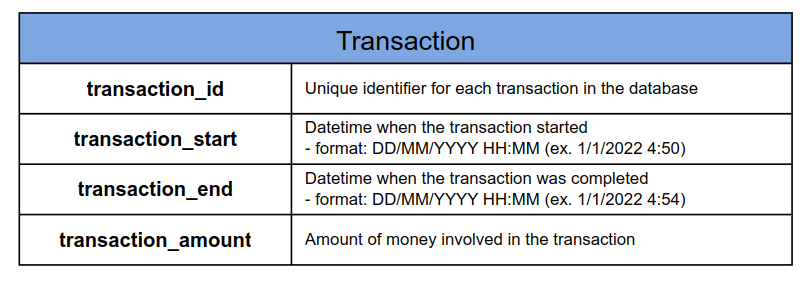
\includegraphics[scale = 0.40]{images/transaction.png}
    \caption{Transaction relation attributes}
    \label{img:pg-stable}
\end{figure}

\end{comment}

The transaction set constitutes the simulated input data stream continuously arriving to the system. Each transaction represents the operation done by a client's card on a ATM of the bank network. Therefore it has the form of a \emph{interaction} edge/relation from the volatile subgraph (see \ref{section:volatile-pg}) matching one Card with one ATM from the stable bank database.

Note that, as in our definition of the input data stream of the $DP_{CQE}$, we will generate two edges per transaction -- the \emph{opening} and the \emph{closing} edge -- which both will constitute a single \emph{interaction} relation. The \emph{opening} edge (Figure \ref{img:opening-edge}) will be the indicator of the begining of a new transaction between the matched Card and ATM, it contains the values of the properties related with the starting time \texttt{start}, the transaction \texttt{type} as well as the \texttt{id}. The \emph{closing} edge (Figure \ref{img:closing-edge}) will indicate the end of the transaction, completing the values of the rest of the properties of the \emph{interaction}: \texttt{end} and \texttt{amount}.


\begin{figure}[h]
  \centering
  \includegraphics[scale = 0.8]{images/2-edges-tx-tfm.png}
  \caption{\emph{Opening} interaction edge}
  \label{img:opening-edge}
\end{figure}

\begin{figure}[h]
  \centering
  \includegraphics[scale = 0.8]{images/2-edges-tx-tfm-1.png}
  \caption{\emph{Closing} interaction edge}
  \label{img:closing-edge}
\end{figure}

We divide the generation of the transaction set in two subsets: the regular transaction set and the anomalous transaction set. The regular transaction set consists of the \emph{ordinary/correct} transactions, whereas the anomalous transaction set is composed of the \emph{irregular/anomalous} transactions that are intentionally created to produce anomalous scenarios.
The main objective under this division is the ability to have the control on the exact number of anomalous ATM transactions that we generate so that we can later measure the efficiency of our system detecting them. \textcolor{gray}{as we have the exact number of anomalous transactions created to compare with, represented by size of the anomalous subset. Otherwise, if we were generating all the transactions together at the same time it would be more difficult to have the control on the amount of anomalous scenarios created, so that later, it will not be possible to measure the efficiency of our system detecting them, since we will not know their amount.}


\textcolor{blue}{To do the generation of the synthetic set of transactions we created the Python program \texttt{transactionGenerator.py}. On it we need to specify the value of the parameters needed to customise the generation of the set of transactions.}

\textcolor{red}{TODO: DEFINE HOW TO RUN IT AND WHICH ARE THE PARAMETERS THAT WE NEED TO INTRODUCE}.

\paragraph{Regular Transaction Set\\}

\begin{tcolorbox}
  \begin{itemize}
    \item \textcolor{green}{$\Rightarrow$}\textbf{By card}: Generation of the transactions for each of the cards independently. \textbf{We have
    control} to avoid anomalous scenarios when selecting the ATMs and distributing the transactions along time.
    \item \textbf{In general}: Linking ATM and client composing (card,ATM) pairs, and distributing these pairs along
    time according to a certain distribution. \textbf{No control / More difficult to control the possible derived
    anomalous scenarios produced among same card pairs}.
  \end{itemize}
\end{tcolorbox}

Therefore, the generation by card option it is considered to be the best so to be able to have the control
on the possible anomalous scenarios for the generated transactions of each of the cards. Some ideas to explore:

\begin{itemize}
  \item Selection of ATMs:
  \begin{itemize}
    \item \textcolor{green}{$\Rightarrow$} Neighborhood / Closed ATM subset.
    \item Random walk. To do the selection of the sequence of ATMs for the generated transactions.
  \end{itemize}
  \item Distribution of the transactions along time:
  \begin{itemize}
    \item \textcolor{green}{$\Rightarrow$} Uniform distribution.
    \item \textcolor{blue}{$\Rightarrow$ (Consider the possibility)} Poisson process distribution.
  \end{itemize}
  \item Other options:
  \begin{itemize}
    \item Random walk for both the ATM and the transaction time selection, in the same algorithm together.
  \end{itemize}
\end{itemize}

\textcolor{red}{TODOS:
\begin{itemize}
\item Cambiar/Actualizar dibujos
\item Poner lista de params y explicar (tabla) como y qué se puede configurar
\item Prerequisitos: csv directory has to exist - create it beforehand better
\item Output files that are generated: regular, anomalous and all csvs.
\item Anomalous generator:
\begin{itemize}
  \item NO-Overlapping assumption - Explain
  \item Any type of tx to produce the fraud -> does not matter the type for the FP1.
\end{itemize}
\end{itemize}
}

The key idea of the transactions of this set is to avoid the creation of anomalous scenarios among them, so to have a close-to-reality simulation of a bank transaction stream flow free of anomalies. After this set is created, the transactions producing anomalous scenarios related with each specific fraud pattern will be produced.


We generate transactions for each of the generated cards on our bank network, based on each of the gathered card transaction behavior. The regular transaction data stream is generated for a customisable \texttt{NUM\_DAYS} number of days starting in a \texttt{START\_DATE}. On what follows we give the details on the procedure done for each of the cards:

\textcolor{gray}{
For a card, the idea is to create a certain 
number of transactions per day, by linking the card to a certain ATM that is no farther 
than \textcolor{orange}{\texttt{max\_distance}} kms from the residence location of the 
client of the card. Also, we will limit the time distance between two consecutive 
transactions so that the final set of created transactions can not produce a potential 
fraud related with having two transactions in different ATM locations with an insufficient 
feasible time distance.
}

\begin{enumerate}
    \item \textbf{Creation of the ATM subset}: Among all the ATMs of the stable bank database we create a subset of ATMs, such that all the regular transactions generated for this card take place in (randomly selected) ATMs of this subset. 
    \textcolor{red}{TODO: ALIGN THIS}
    $$\texttt{ATM\_subset} = \{\texttt{ATM}\ \\
    |\ \texttt{distance(ATM,residence\_loc)} \leq \texttt{MAX\_DISTANCE\_SUBSET\_THRESHOLD}\}$$

    \texttt{ATM\_subset} consists of the ATMs that are considered to be \textit{usual} for the card, considering the ATMs that are at a distance lower or equal to a customisable maximum distance threshold \texttt{MAX\_DISTANCE\_SUBSET\_THRESHOLD} to the registered residence location \texttt{residence\_loc} on the card. We also limit the size of this subset, considering only a maximum ratio of the total number of ATMs (\texttt{MAX\_SIZE\_ATM\_SUBSET\_RATIO} $\in [0,1]$), so that only a certain ratio of the closest ATMs are included on it.

    $$|\texttt{ATM\_subset}| = \texttt{MAX\_SIZE\_ATM\_SUBSET\_RATIO} * |\texttt{ATM}|$$

\textcolor{red}{TODO: CAMBIAR ESTA IMAGEN}
    \begin{figure}[H]
      \centering
      \includegraphics[scale=1.1]{images/tx-generation-1-named.png}
      \caption{\texttt{Neighborhood} ATM subset}
    \end{figure}

    \item \textbf{Calculate \texttt{t\_min\_subset}}: Minimum threshold time between any two consecutive transactions of the card. That is, the minimum time distance between the end of a transaction and the start of the next consecutive transaction of a card. For it, we take the time needed to traverse the maximum distance between any pair of ATMs of the \texttt{ATM\_subset}: \texttt{max\_distance\_subset} at an assumed speed that any two points can be traveled for the case of ordinary scenarios: \texttt{REGULAR\_SPEED}.
    $$\texttt{t\_min\_subset} = \frac{\texttt{max\_distance\_subset}}{\texttt{REGULAR\_SPEED}}$$

    \item \textbf{Decide the number of transactions \texttt{num\_tx}}:
    Based on the behavior of the card, we decide the number of transactions (\texttt{num\_tx}) to generate for the card for the selected number of days \texttt{NUM\_DAYS} as:

    $$\texttt{num\_tx} \sim \text{Poisson}(\lambda = \texttt{ops\_day} * \texttt{NUM\_DAYS})$$ where \texttt{ops\_day} is the sum of the average number of all the kinds of operations per day of the particular card: 
    $$\texttt{ops\_day} = \texttt{withdrawal\_day} + \texttt{ deposit\_day} + \texttt{ inquiry\_day} + \texttt{ transfer\_day}$$


    \item \textbf{Decide on the type of transaction}: for each of the \texttt{num\_tx} transactions, the transaction \texttt{type} is decided randomly assigning a transaction \texttt{type} given a probability distribution constructed from the card behavior:
    
    $$
    \begin{cases}
      P(\texttt{type} =  \texttt{withdrawal}) = \frac{\texttt{withdrawal\_day}}{\texttt{ops\_day}} \\[8pt]
      P(\texttt{type} =  \texttt{deposit}) = \frac{\texttt{deposit\_day}}{\texttt{ops\_day}} \\[8pt]
      P(\texttt{type} = \texttt{inquiry}) = \frac{\texttt{inquiry\_day}}{\texttt{ops\_day}} \\[8pt]
      P(\texttt{type} =  \texttt{transfer}) = \frac{\texttt{transfer\_day}}{\texttt{ops\_day}} 
    \end{cases}
    $$

    \item \textbf{Distribution of the \texttt{num\_tx} transaction times}: along the selected number of days \texttt{NUM\_DAYS} time interval.
    
    We do a random uniform distribution of the \texttt{num\_tx} transaction times
    in the time interval starting in \texttt{START\_DATE} and finishing \texttt{NUM\_DAYS} days after, obtaining the \texttt{start} and \texttt{end} times for each of the \texttt{num\_tx} transactions, with the constraint that, for each transaction $i$, the next one $i+1$ is at a minimum time distance of \texttt{t\_min\_subset}. Specifically, the transaction times are generated guaranteeing:

    $$i.\texttt{end} + \texttt{t\_min\_subset} < (i+1).\texttt{start} \ \forall i \in [1,\texttt{num\_tx})$$

    The \texttt{end} time of a transaction is assigned a shifted time difference with respect to the \texttt{start} time. In particular:

    $$
    \texttt{end} = \texttt{start} + \texttt{time\_difference}
    $$

    where:

    $$\texttt{time\_difference} \sim \mathcal{N}(\texttt{MEAN\_DURATION},\,\texttt{STD\_DURATION})$$ with the corrections:

    $$
    \texttt{time\_difference} =
    \begin{cases} 
        \texttt{MEAN\_DURATION} & \text{if } \texttt{time\_difference} < 0 \\
        \texttt{MAX\_DURATION} & \text{if } \texttt{time\_difference} > \texttt{MAX\_DURATION} \\
        \texttt{time\_difference} & \text{otherwise}
    \end{cases}
    $$

\textcolor{red}{TODO: PONER UN DIBUJITO!, explicar lo del checking de los fitting holes? --> yo creo que esto ya no es necesario... demasiado detalle}


  \item Assign a transaction \texttt{amount}: assigned depending on the \texttt{type} based on card behavior:
    
  $$
  \begin{cases}
    \mathcal{N}(\texttt{amount\_avg\_withdrawal},\, \texttt{amount\_std\_withdrawal}) & \text{if } \texttt{type} = \texttt{withdrawal} \\[10pt]
    
    \mathcal{N}(\texttt{amount\_avg\_deposit},\, \texttt{amount\_std\_deposit}) & \text{if } \texttt{type} = \texttt{deposit} \\[10pt]

    0 & \text{if } \texttt{type} = \texttt{inquiry} \\[10pt]
    
    \mathcal{N}(\texttt{amount\_avg\_deposit},\, \texttt{amount\_std\_transfer}) & \text{if } \texttt{type} = \texttt{transfer}
  \end{cases}
  $$

  $$
  \text{If } \texttt{amount} < 0, \text{ then re-draw from } U(0, 2 \cdot \texttt{amount\_avg\_type}).
  $$

  with \texttt{amount\_avg\_type} as \texttt{amount\_avg\_withdrawal}, \texttt{amount\_avg\_deposit} or \texttt{amount\_avg\_deposit} depending on the respective transaction \texttt{type}.

\end{enumerate}

As a summary we show a pseudocode of the transaction generator in Algorithm \ref{alg:regular-tx-generator}.

\begin{algorithm}[H]
  \small
  \begin{algorithmic}[1]
  \STATE $\texttt{id} \gets 0$
  \FOR{\text{card} in \text{cards}}
    \STATE $\texttt{ATM\_subset}, \overline{\texttt{ATM\_subset}} \gets \text{createATMsubset(\texttt{residence\_loc})}$
    \STATE $\texttt{t\_min\_subset} \gets \text{calculate\_t\_min\_subset(\texttt{ATM\_subset})}$
    \STATE $\texttt{num\_tx} \gets \text{decide\_num\_tx()}$
    \STATE $T \gets \text{distribute}(\texttt{num\_tx}, \texttt{t\_min\_subset})$
    \FOR{$t_i$ in $T$}
        \STATE $\texttt{ATM}_{i} \sim \texttt{ATM\_subset}$
        \STATE $\texttt{start}_{i} \gets t_i.start$
        \STATE $\texttt{end}_{i} \gets t_i.end$
        \STATE $\texttt{type}_{i} \gets \text{getType()}$
        \STATE $\texttt{amount}_{i} \gets \text{getAmount()}$
        \STATE $\texttt{id}_{i} \gets \texttt{id}; \ \texttt{id} \gets \texttt{id} + 1$
        \STATE $\text{createTransaction}(\texttt{id}_{i}, \texttt{ATM}_i, \texttt{start}_{i},\texttt{end}_{i}, \texttt{type}_{i}, \texttt{amount}_i)$
    \ENDFOR
    \STATE $\text{introduceAnomalous}(\texttt{ATM\_subset}, \overline{\texttt{ATM\_subset}})$
  \ENDFOR
  \end{algorithmic}
  \caption{Regular Transactions Generation}
  \label{alg:regular-tx-generator}
\end{algorithm}

\textcolor{red}{TODO: PONER NOMBRES DE LAS FUNCIONES EMPLEADAS - REFERENCIAS EN EL TEXTO DE LA EXPLICACIÓN DE ARRIBA!}

\paragraph{Anomalous Transaction Set\\}

After the generation of regular transactions we perform an injection of transactions to produce anomalous scenarios. The injection is taylored depending on the specific kind of 
anomalous scenarios that we want to produce. In what follows we explain the injection process depending on each of the types of frauds that we have considered.

\paragraph{Fraud Pattern I}

To produce anomalous scenarios related to this type of fraud, we produce the injection
of transactions that will produce the satisfaction of this fraud pattern. In other words,
we inject transactions that violate the minimum \emph{time-distance} constraint between transactions performed with the same card. Therefore, as we can see in Figure \ref{img:anomalous-type-1}, if we consider a set of regular transacions for a certain card, where $y_1$ and $y_2$ are regular consecutive transactions, we will introduce an anomalous transaction $a_{12}$ such that: 

$$(y_1.\texttt{ATM\_id} \ne a_{12}.\texttt{ATM\_id}) \land (a_{12}.\texttt{start} - 
y_1.\texttt{end} < T_{min}(y_1.\texttt{ATM\_loc}, a_{12}.\texttt{ATM\_loc}))$$

where \texttt{ATM\_loc} is the tuple of coordinates (loc\_latitude,loc\_longitude) of the corresponding ATM. This injection will produce an anomalous scenario of this kind of fraud with at least the $y_1$ previous transaction. Note that, it could possibly trigger more anomalous fraud scenarios with the subsequent transactions ($y_2$ and on...).

\begin{figure}[H]
    \centering
    \includegraphics[width=\textwidth]{images/tx-generation.png}
    \caption{Creation of anomalous scenario - type I}
    \label{img:anomalous-type-1}
\end{figure}

Some assumptions related with the generation of anomalous transactions for this kind of fraud pattern are:
\begin{itemize}
  \item \textbf{Overlapping of transactions is not possible}:
  Appart from guaranteeing that this injection causes at least one anomalous scenario, we also respect the additional constraint of ensuring that the anomalous transaction injected does not cause overlapping with any of the transactions, in particular neither with the previous nor the next one. \textcolor{orange}{This constraint is added based on the assumption that the bank itself does not allow to open a transaction whenever another one is still open.} Therefore considering that $a_{12}$ is the anomalous injected transaction in between the regular consecutive transactions $y_1$ and $y_2$, when generating $a_{12}$ we guarantee that:
  $$
  \begin{cases}
    a_{12}.\texttt{start} > y_{1}.\texttt{end} \\
    a_{12}.\texttt{end} < y_{2}.\texttt{start}
  \end{cases}
  $$
  \item \textbf{There are no two consecutive anomalous transactions}: For simplicity in our practical purposes, we do the generation of anomalous transactions for this kind of fraud pattern assuming that an anomalous transaction can only be in between two regular consecutive transactions, so that we do not consider the case of the injection of two or more consecutive anomalous transactions for this kind of fraud. See Figure \ref{img:anomalous-type-1-insertion-points}.
  \begin{figure}[H]
    \centering
    \includegraphics[width=\textwidth]{images/tx-generation-anomalous-1.png}
    \caption{Considered possible injection points of anomalous transactions of fraud type I}
    \label{img:anomalous-type-1-insertion-points}
  \end{figure}  
\end{itemize}

We generate $\texttt{ANOMALOUS\_RATIO\_1} * \texttt{num\_tx}$ anomalous transactions for each of the cards related with the fraud pattern I, where $\texttt{ANOMALOUS\_RATIO\_1} \in [0,1]$ defines the ratio of anomalous transactions of this kind over the total number of regular transactions \texttt{num\_tx} for each of the cards. In Algorithm \ref{alg:anomalous-tx-generator-1} we describe at a high level the process of the generation of anomalous transactions for this kind of fraud pattern. 


\textcolor{red}{Preconditions:
\begin{itemize}
  \item ATMsubset, and the compl. are given by param, from the tx regular generator
\end{itemize}
}

\begin{algorithm}[H]
  \small
  $\textbf{introduceAnomalous}(\texttt{ATM\_subset}, \overline{\texttt{ATM\_subset}})$
  \begin{algorithmic}[1]
  \STATE $\texttt{num\_anomalous} \gets \texttt{num\_tx} * \texttt{ANOMALOUS\_RATIO\_1}$
  \STATE $i \gets 0$
  \WHILE{$i < \texttt{num\_anomalous}$}
      \STATE $\texttt{ATM}_{i} \sim \overline{\texttt{ATM\_subset}}$
      \STATE $prev_i, next_i \gets \text{randomUniquePosition(\texttt{num\_tx})}$
      \STATE $t_i \gets \text{getTime}(prev_i, next_i)$
      \STATE $\texttt{start}_{i} \gets t_i.start$
      \STATE $\texttt{end}_{i} \gets t_i.end$
      \STATE $\texttt{type}_{i} \gets \texttt{getRandomType()}$
      \STATE $\texttt{amount}_{i} \gets \texttt{getAmount()}$
      \STATE $\texttt{id}_{i} \gets \texttt{id}; \ \texttt{id} \gets \texttt{id} + 1$
      \STATE $\texttt{createTransaction}(\texttt{id}_{i}, \texttt{ATM}_i, \texttt{start}_{i},\texttt{end}_{i}, \texttt{type}_{i}, \texttt{amount}_i)$
      \STATE $i \gets i + 1$
  \ENDWHILE
  \end{algorithmic}
  \caption{Introduction of Anomalous Transactions for Fraud Pattern I}
  \label{alg:anomalous-tx-generator-1}
\end{algorithm}


\begin{enumerate}
  \item \textbf{Assignment of ATMs not belonging to the \texttt{ATM\_subset}}: the anomalous transactions are linked to ATMs that are part of the complementary of the \texttt{ATM\_subset}.
  \item \textbf{Each anomalous transaction has a unique insertion position}: As described previously, we do not allow the case of two or more consecutive anomalous transactions injection. Each anomalous transaction occupies a unique position among all the possible injection positions defined by the set of regular transactions generated for the card. As it can be seen on Figure \ref{img:anomalous-type-1-insertion-points}, considering that we have three regular transactions, we will consider three unique possible insertion points for the anomalous transactions. The procedure of assigning a unique insertion position for each anomalous transaction to be generated is achieved with the function \text{randomUniquePosition(\texttt{num\_tx})}, that given the number of regular transactions of the card \texttt{num\_tx} returns the previous and the next regular transaction to the assigned unique position.
  \item \textbf{Assign transaction times such that respecting the needed time constraints}: in particular there are two time constraints to be satisfied:
  \begin{itemize}
    \item Production of fraud pattern with prev\_i
    \item No overlapping with prev\_i nor with next\_i
  \end{itemize}
  This is summarized in the pseudocode as the procedure getTime(prev\_i, next\_i), which returns $t_i$, as the tuple of (\texttt{start},\texttt{end}) times.
  \item \textbf{Random transaction type}
  \item \textbf{Arbitrary amount}
 
\end{enumerate}


\textcolor{red}{TODO: MENCIONAR MÁS COSAS EN UN LISTADO, COMO EN LA GENERACIÓN DE TX REGULARES?!}

\begin{comment}
\subsubsection{ATM closed subset + Poisson Process}

\begin{tcolorbox}
  \begin{itemize}
    \item[$\rightarrow$] \textbf{ATM selection}: Closed ATM subset.
    \item[$\rightarrow$] \textbf{Time distribution}: Poisson process distribution of $num\_tx$ 
    transactions for each of the cards.
  \end{itemize}
\end{tcolorbox}

Generate $\texttt{num\_tx}$ transactions for a selected period of time $\texttt{t}$.
Distribution following a Poisson process distribution along $[0,t]$.
\begin{itemize}
    \item[$\bullet$] $\lambda=\texttt{avg\_tx}$ on a day for the client if $\texttt{t = 24h}$. Otherwise, 
    decide a specific $\lambda$ for the considered $\texttt{t}$.
    \item[$\bullet$] Inter-arrival times $X_1, X_2, \cdots$ are distributed following an exponential distribution:
    $X_i \sim \text{Exp}(\lambda)$. They represent the time elapsed between two of these events, e.g. $X_2$ represents the time elapsed between the first and the second arrival. Note that in this case, since we need to respect the minimum required time between two consecutive 
    transactions ($t_{min}$) so to avoid introducing anomalous undesired scenarios, we have to impose
    that: $X_i \geq \Delta_{i-1} + t_{min}, \forall X_i$, where:

    \begin{itemize}
      \item[$\circ$] $X_{i}$: time elapsed between the $i$-$1$ and $i$-th transaction.
      \item[$\circ$] $\Delta_{i-1}$: time duration of the $i$-$1$ transaction. This duration will 
      be upper bounded by $\Delta_{max}$, which will be considered the maximum possible duration of a transaction.
      \item[$\circ$] $t_{min}$: minimum calculated time distance between any 2 consecutive transactions of the client.
  \end{itemize}

    With these interarrival times, we obtain the arrival times $T_i$. Note that they are not independent, in particular:
    $T_1 \leq T_2 \leq T_3 \cdots$.

    Therefore, to generate the Poisson process with rate $\lambda$:
    \begin{enumerate}
      \item Generate i.i.d. random variables $X_1, X_2, \cdots$ where $X_i \sim \text{Exp}(\lambda)$.
      \item Obtain the arrival times as:
        \begin{itemize}
          \item $T_1 = X_1$
          \item $T_2 = X_1 + X_2$
          \item $T_3 = X_1 + X_2 + X_3$
          \item $\cdots$
        \end{itemize}
    \end{enumerate}

    Note that, having imposed the previous we will have that:
    \begin{equation}
      \begin{cases}
        T_i = T_{i-1} + X_i \\
        X_i \geq \Delta_{max} + t_{min}
      \end{cases}\forall X_i \
    \end{equation}

    which implies that:
    
    \begin{equation}
      T_i \geq T_{i-1} + \Delta_{max} + t_{min}, \forall X_i
    \end{equation}
    
\end{itemize}
\begin{figure}[H]
    \centering
    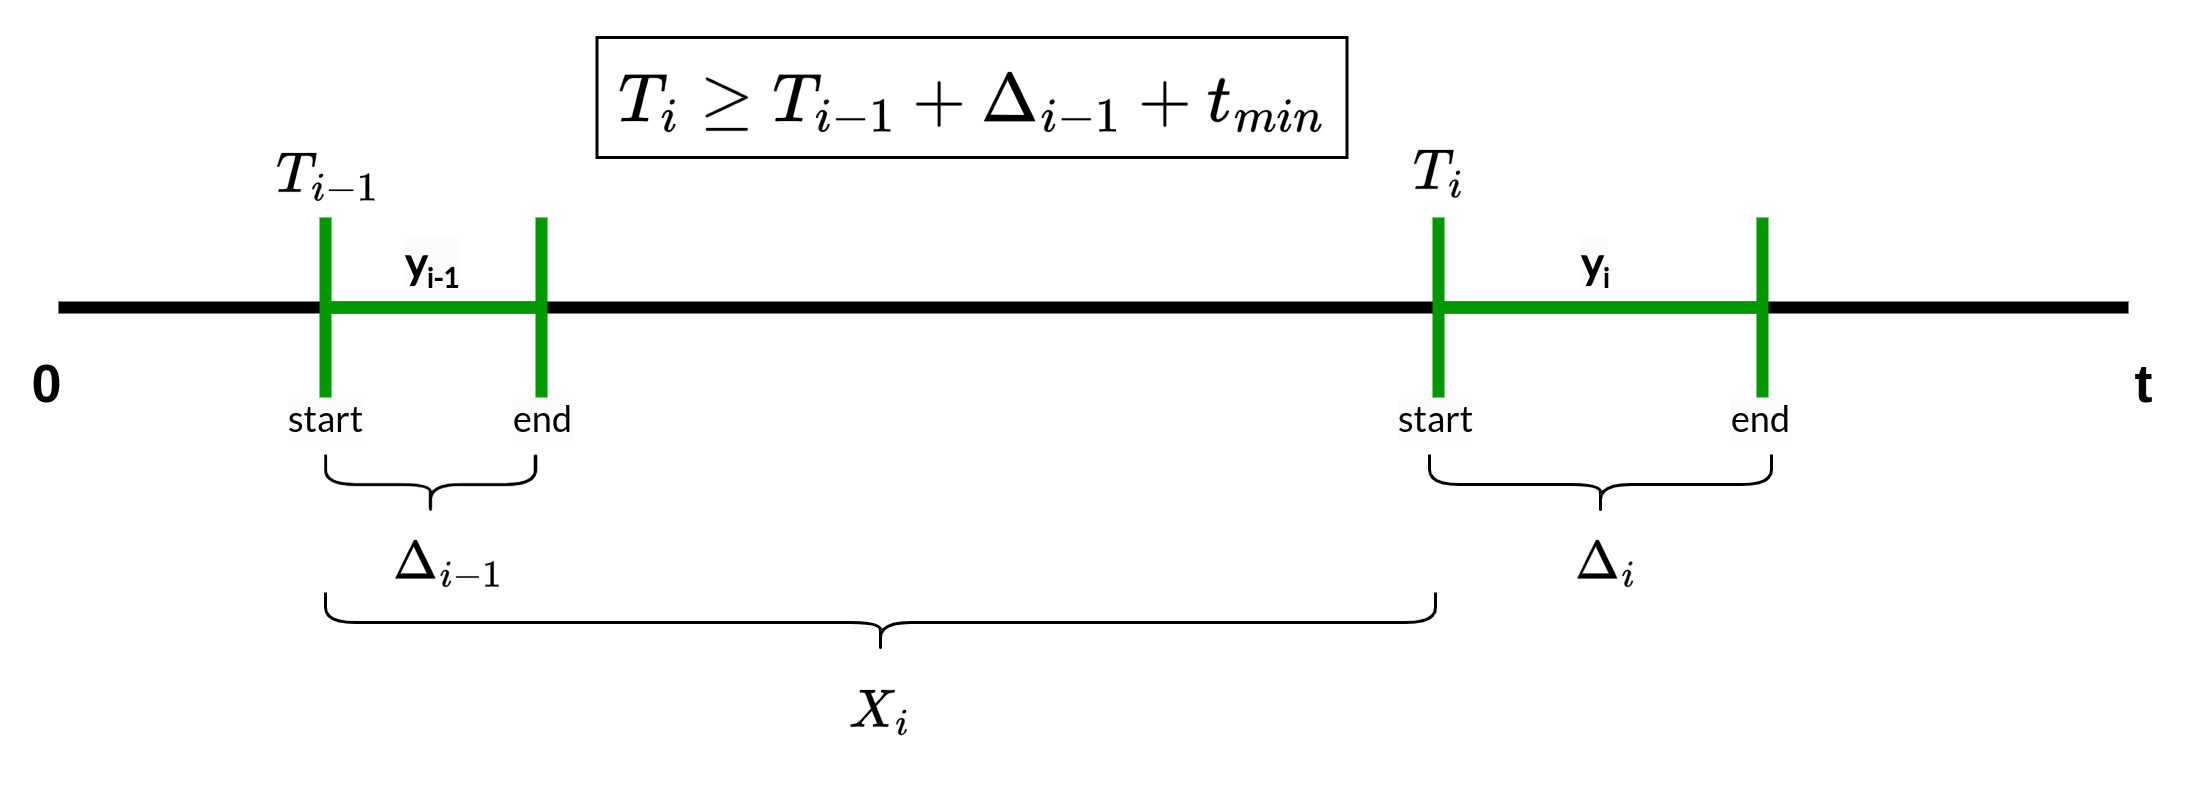
\includegraphics[scale=0.55]{images/tx-generation-dist-corrected.png}
    \caption{Schema of the interarrival and arrival event times on the poisson process.}
\end{figure}


References:

\begin{itemize}
  \item \href{https://www.probabilitycourse.com/chapter11/11_1_2_basic_concepts_of_the_poisson_process.php}{Poisson process modeling - Theoric description}
  \item \href{https://www.probabilitycourse.com/chapter14/Chapter_14.pdf}{Poisson process modeling - Python implementation}
  \item \href{https://timeseriesreasoning.com/contents/poisson-process/}{Less formal explanation with Python code}
  \item \href{https://www.math.wsu.edu/faculty/genz/416/lect/l05-45.pdf}{More theory}
  \item \href{https://en.wikipedia.org/wiki/Poisson_point_process}{Wikipedia entry}
\end{itemize}

\subsubsection{Random Walk / Markov Chain}

Idea is to model the sequence of transactions for each of the clients as a markov chain through the
network of ATMs. The network is a fully-connected graph with ATMs as nodes and edges are
weighted with the distance between each pair of ATMs as weights.

The idea is to obtain the sequence of transactions for each client as a markov chain, in which,
for each step a transaction is generated in that specific ATM node, at a certain datetime 
respecting the constraint of the minimum time distance with the previous transaction, so 
that no undesired anomalous fraud scenarios are produced. \\ 

Some considerations:
\begin{itemize}
  \item Initially, we will compute the transition matrix obtaining all the respective 
  transition probabilities. The probability of transition to another ATM-node will be 
  inversely proportional to the distance to the considered ATM-node.
  \item Transition matrix $P_t$: containing, for each state, the probability of transitioning
  between states. For example, the entry $i,j$: $(P_t)_{i,j} = \mathcal{P}(X_{t+1} = j | X_t = i)$
  contains the probability of transitioning to state $j$ when being in state $i$. 
  Note that since we assume a complete graph, and also the posibility to transition 
  to the same state, all entries of this matrix will be distinct to 0: $(P_t)_{i,j} \neq 0 \  
  \forall i,j$.
  \item Finally, once $P_t$ is computed, we perform the simulation to obtain the sequence of
  transactions for the specific card/client.
\end{itemize}

References:

\begin{itemize}
\item Markov Chains
\begin{itemize}
  \item \href{https://brilliant.org/wiki/markov-chains/}{MC - Theory}
  \item \href{https://www.columbia.edu/~ks20/4703-Sigman/4703-07-Notes-MC.pdf}{Simulation of Markov Chains - Theory}
  \item \href{https://stephens999.github.io/fiveMinuteStats/simulating_discrete_chains_1.html}{MC - Implementation example}
  \item \href{https://www.youtube.com/watch?v=G7FIQ9fXl6U}{MC - Implementation video example}
\end{itemize}
\item Random Walks
\begin{itemize}
  \item Theory:
  \begin{itemize}
    \item \href{https://ieeexplore.ieee.org/abstract/document/8911513?casa_token=vznpjKL5HG0AAAAA:hNzLCxAHBk75zCDUHsswB7ImAKgilzZcOBzxaXWz_G6U8Vy-ogbei40MoZ49M-Em5tTii0Q}{RWs: A Review of Algorithms and Applications}
    \item \href{https://www.lirmm.fr/~sau/JCALM/Josep.pdf}{RWs on Graphs}
    \item \href{https://www.fi.muni.cz/usr/gruska/random18/random1808.pdf}{RW - More theory}
  \end{itemize}
  \item Implementation examples:
  \begin{itemize}
    \item \href{https://tleise.people.amherst.edu/Math365Spring2016/RmarkdownFiles/WalkOnGraph.html}{Simple RW on a Graph - Implementation example}
    \item \href{https://graphstream-project.org/doc/Algorithms/Random-walks-on-graphs/}{A RW on a graph - Implementation}
    \item \href{https://es.mathworks.com/help/econ/simulate-random-walks-through-markov-chain.html}{Simulate Random Walks Through Markov Chain - Matlab Implementation example}
  \end{itemize}
\end{itemize}
\end{itemize}
\end{comment}


\textcolor{gray}{
Regarding the data model, the new nature of data requires a de facto new database paradigm
-continuously evolving databases- where data can be both stable and volatile. Even though
evolving databases can be implemented according to any approach, graph databases seem
especially well suited here [1, 2]. Indeed, the natural way to process evolving graphs as streams
of edges gives insights on how to proceed in order to maintain dynamic graph databases. Hence,
we consider that a suitable data model is a continuously evolving data graph, a graph having
persistent (stable) as well as non persistent (volatile) relations. Stable relations correspond
to edges occurring in standard graph databases while volatile relations are edges arriving indata streams during a set time interval. Once this time interval is over, the relations are not
longer valid so that there is no need to store them in the (stable) graph database. However,
when required -as for further legal or auditing purposes- timestamped occurrences of volatile
relations can be kept in a log file. Volatile relations induce subgraphs that exist only while the
relations are still valid. Without loss of generality, in this work we consider property graphs
(PG) [3, 4] as the basic reference data model. As an example, Figure 1a depicts part of a schema
of a PG database where stable relations correspond to the data that a bank typically gathers
on its issued cards, ATMs (Automated Teller Machines) network, etc. Volatile relations model
the interaction between cards and ATM entities}


\textcolor{blue}{In the context of our work we could see the data we are considering to be both static and streaming data, as we are considering a bank system application that contains all the information related to it on the cards, clients\dots, and that it is receiving the streaming of transactions that happens on it.
More specifically, the static data can be thinked of the classical bank database data, that is, the data a bank typically gathers on its issued cards, clients, accounts, ATMs\dots. Whereas as the streaming data we can consider the transactions the clients of the bank produce with their cards on ATMs, PoS\dots that reach the bank system.
Therefore, due to this nature of the data, we consider a \emph{continuously evolving database} paradigm, where data can be both stable and volatile. Even though 
evolving databases can be implemented according to any approach, graph databases seem especially well suited here \textcolor{blue}{\cite{angles2008survey, kumar2015graph}}. 
% TODO: PONER REFERENCIAS
% TODO: PONER + RAZONES?
}


The property graph data model consists of two sub property graphs: a stable and a volatile property graph. On the one hand, the stable is composed of the static part of the data that a bank typically gathers such as information about its clients, cards, ATMs (Automated Teller Machines). 
On the other hand, the volatile property graph models the transaction operations, which defines the most frequent and reiterative kind of interaction between entities of the data model.\\
The main difference and the main reason for this separation is the semantics with which we intentionally define each of the subgraphs: the stable will be understood like a fixed static bank database, whereas the volatile will be understood as the data model to define the transactions, as continuous interactions between the entities of the model, which will not be permanently saved, but instead, only for a certain window of time under the mission of detecting anomalous bank operations. Note that we will only model the transaction interaction in the volatile subgraph, only letting them occur here.
This separation will allow us to have a really simple and light property graph schema single-centered on the transactions with the minimal needed information (mostly identifiers of the entities a transaction links) and another, the stable, acting as a traditional bank database schema, from which to obtain the information details of the entities.

\textcolor{gray}{Due to the confidential and private nature of bank data, it was
impossible to find a real bank dataset nor a real bank data model. Therefore, we developed our own proposal of a bank database model.}

\subsection{Design of the Data Model}

In what follows we describe the design of our data model as a Property Graph data model, divided into the stable and volatile property graphs. Due to the confidential and private nature of bank data, it was impossible to find a real bank dataset nor a real bank data model. In this regard, we developed our own proposal of a bank database model taking as standard reference the \emph{Wisabi Bank Dataset}\footnote{https://www.kaggle.com/datasets/obinnaiheanachor/wisabi-bank-dataset}, which is a fictional banking dataset publicly available in the Kaggle platform.

\subsubsection{Stable Property Graph}\label{section:stable-pg}

Taking into account the reference dataset model, a common bank data model could be the one we defined in Figure \ref{img:pg-stable-big}, which intents to capture the data that a bank system database typically gathers.\\
It contains four entities: Bank, ATM, Client and Card with their respective properties, and the corresponding relationships between them. The relations are: a directed relationship from Client to Card \texttt{owns} representing that a client can own multiple credit cards and that a card is owned by a unique client, then a bidirectional relation \texttt{has\_client} between Client and Bank; representing bank accounts of the clients in the bank. The relation between Card and Bank to represent that a card is \texttt{issued\_by} the bank, and that the bank can have multiple cards issued. Finally, the relations \texttt{belongs\_to} and \texttt{interbank} between the ATM and Bank entities, representing the two different kinds of ATMs depending on their relation with the bank; those ATMs owned and operated by the bank and those that, while not owned by the bank, are still accessible for the bank customers to perform transactions.

\begin{figure}[h]
  \centering
  \includegraphics[scale = 0.7]{images/1-DataModel/PG-stable-edit-cardinal.png}
  \caption{Initial bank stable property graph model}
  \label{img:pg-stable-big}
\end{figure}

Although this data model is quite close to reality, we chose a simplified version of it as the final model for our proof of concept (see Figure \ref{img:pg-stable-def}). On this final version the defined entities, relations and properties modeling the bank database are reduced to the essential ones, which, we believe are enough to create a relevant and representative bank data model sufficient for the purposes of our work.

\begin{figure}[h]
  \centering
  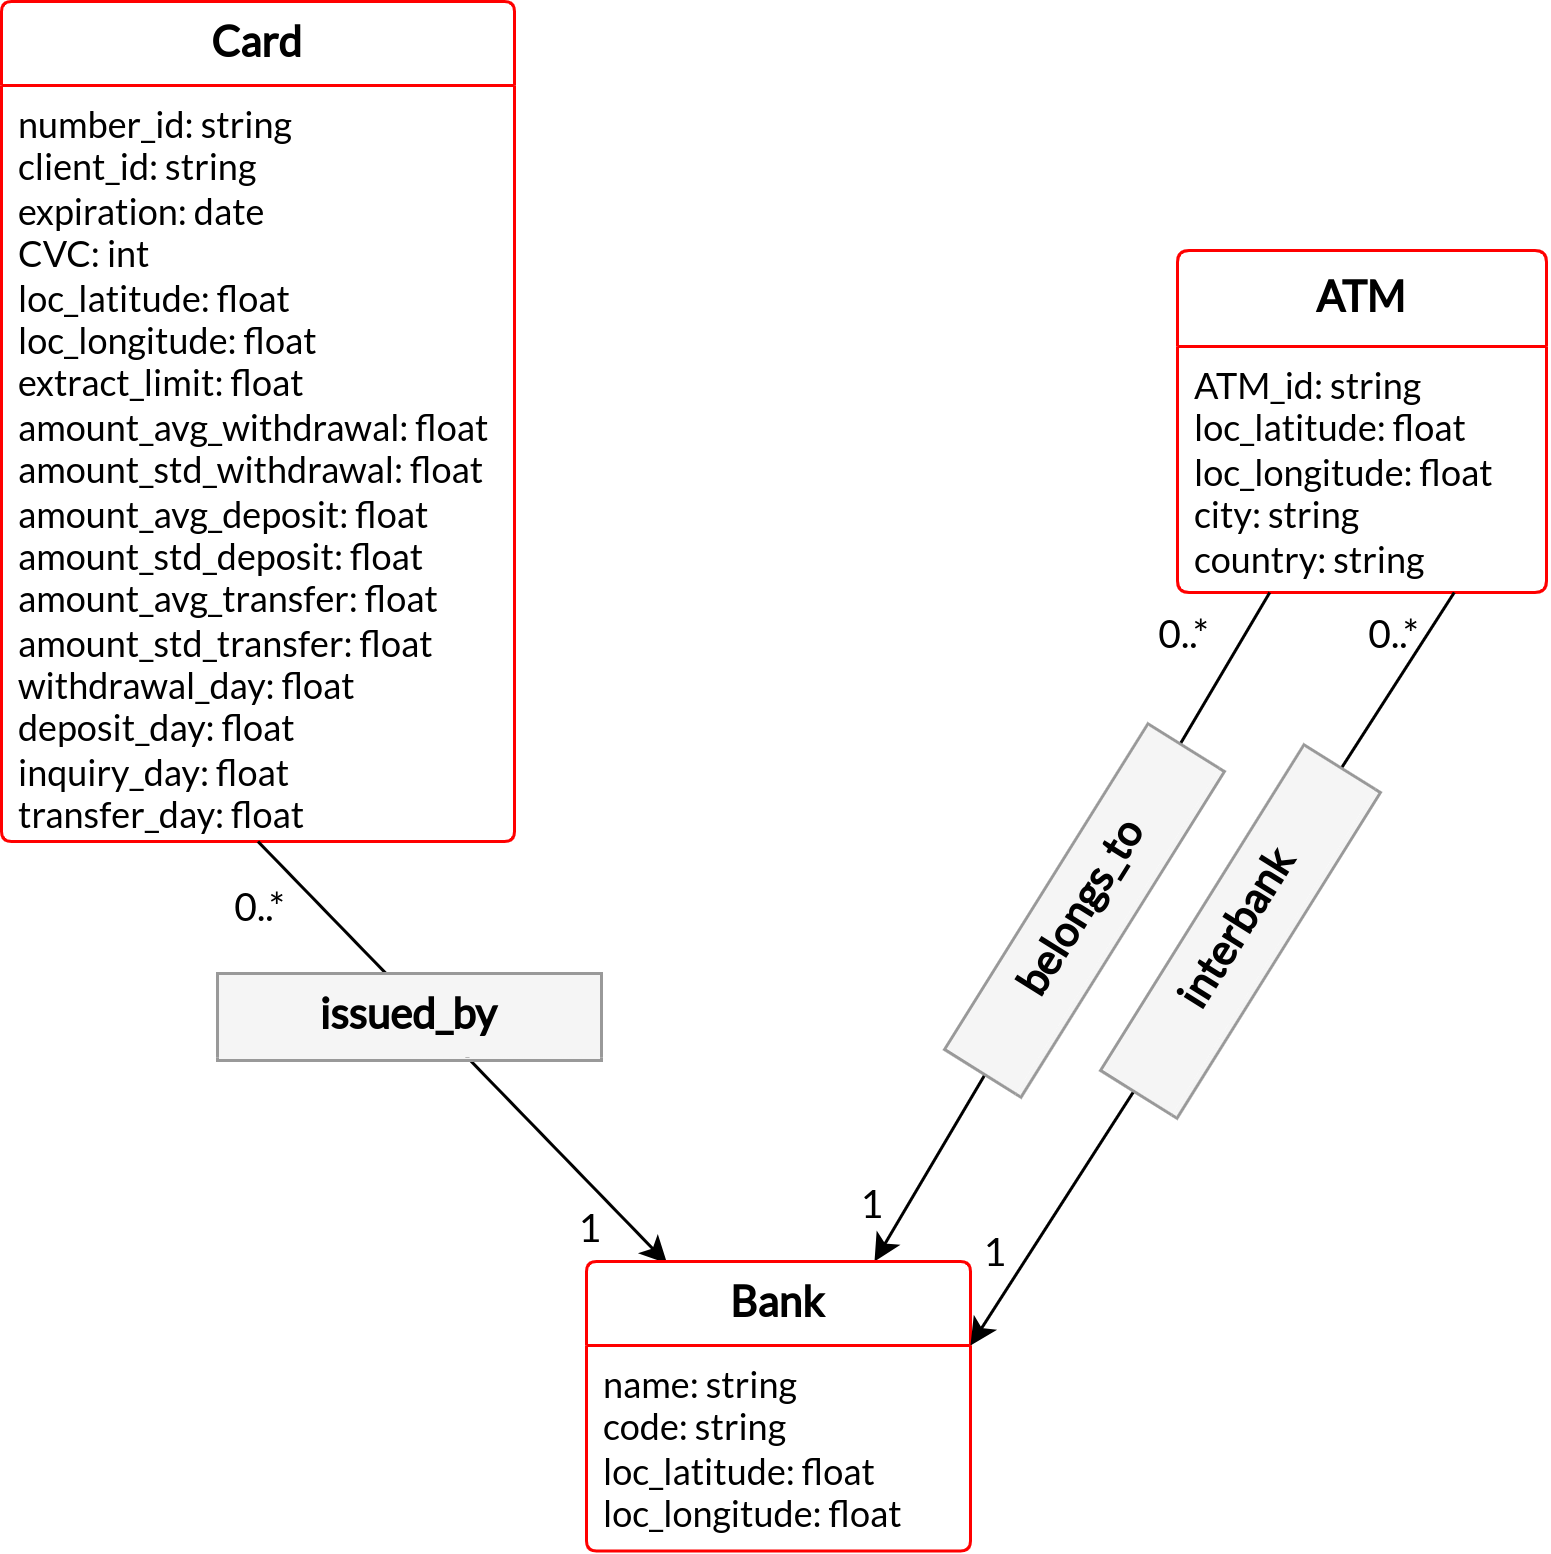
\includegraphics[scale = 0.7]{images/1-DataModel/PG-stable-behavior-cards.png}
  \caption{Definitive stable property graph model}
  \label{img:pg-stable-def}
\end{figure}

On the final version of the model, we decided to remove the Client entity and to merge it inside the Card entity. For this, all the Client properties were included in the Card entity. In the complete data model schema (Figure \ref{img:pg-stable-big}) the Client entity was defined with three properties: the identifier of the client and the GPS coordinates representing the usual residence of the client. This change is done while preserving the restriction of a Card belonging to a unique client the same way it was previously done with the relation between Card and Client \texttt{owns} in the complete schema, which now is therefore removed. \\
% Account relation removed
Another derived consequence of this simplification is the removal of the other relation that the Client entity had with other entities: the \texttt{has\_client} relation between Client and Bank, which was made with the intention of representing the bank accounts between clients and banks. Maintaining a bank account would imply having to consistently update the bank account state after each transaction of a client, complicating the model. Nevertheless, we eliminate the bank account relation, since its removal is considered negligible and at the same time helpful for the simplification of the model needed for the purposes of our work. % Properties included with the purpose of detecting frauds 
However, for the sake of completeness the property \textit{extract\_limit} is introduced in the Card entity, representing a money amount limit a person can extract, which will be related with the amount of money a person owns. This will allow the detection of anomalies related with frequent or very high expenses. Other properties that are included with the purpose of allowing the detection of some other kinds of anomalies are the GPS coordinates and the client's \emph{behavior} properties. The GPS coordinates are added in the ATM and Card entities, in the first case referring to the geolocation of each specific ATM and in the last case referring to each specific client address geolocation. The client's \emph{behavior} properties are added in the Card entity. They are metrics representing the behavior of the owner of the Card, and they are included as properties as we think they could be of interest to allow the detection of some kinds of anomalies in the future.

As a result, our final simplified stable property graph model contains three node entities: Bank, Card and ATM, and three relations: \texttt{issued\_by} associating Card entities with the Bank entity, and \texttt{belongs\_to} and \texttt{interbank} associating the ATM entities with the Bank entity. 

The Bank entity represents the bank we are considering in our system. Its properties consist
on the bank \emph{name}, its identifier \emph{code} and the location
of the bank headquarters, expressed in terms of \emph{latitude} and \emph{longitude}
coordinates, as seen in Table \ref{table:bank-node-properties}.
  
\begin{table}[H]
    \centering
      \begin{tabular}{|l|l|}
      \hline
      \textbf{Name}        & \textbf{Description and value}                                      \\ \hline
      \texttt{name}         & Bank name                                                 \\ \hline
      \texttt{code}         & Bank identifier code                                      \\ \hline
      \texttt{loc\_latitude}  & Bank headquarters GPS-location latitude                   \\ \hline
      \texttt{loc\_longitude} & Bank headquarters GPS-location longitude                  \\ \hline
      \end{tabular}
    \caption{Bank node properties}
    \label{table:bank-node-properties}
\end{table}

\begin{tcolorbox}
\textcolor{red}{Note that, from the beginning we were considering more than 1 bank entity. This lead to consider the creation of this entity, which now as only 1 bank is considered it may not be needed anymore, being able to reformulate and simplify the model. However, it is left since we considered it appropiate to be able to model the different kinds of ATMs a bank can have with different relation types instead of with different ATM types.}
\end{tcolorbox}

The ATM entity represents the Automated Teller Machines (ATM) that either belong to the bank's network or that the bank can interact with.
% Potential possible generalization of the ATM entity to a POS entity
For the moment, this entity is understood as the classic ATM, however note that this entity could potentially be generalized to a Point Of Sale (POS), allowing a more general kind of interactions apart from the current Card-ATM interaction, where also online transactions could be included apart from the physical ones. We distinguish two different kinds of ATMs, depending on their relation with the bank:

\begin{itemize}
  \item Internal ATMs: ATMs owned and operated by the bank. They are fully integrated within the
  bank's network. Modeled with the \texttt{belongs\_to} relation.
  \item External ATMs: These ATMs, while not owned by the bank, are still accessible for the bank
  customers to perform transactions. Modeled with the \texttt{interbank} relation. 
\end{itemize}

Both types of ATMs are considered to be of the same type of ATM node. Their difference
is modeled as their relation with the bank instance: \texttt{belongs\_to} for the internal ATMs and \texttt{interbank} for the external ATMs.

\begin{table}[H]
    \centering
    \begin{tabular}{|l|l|}
    \hline
    \textbf{Property}        & \textbf{Description}                                      \\ \hline
    \texttt{ATM\_id}      & ATM unique identifier                             \\ \hline
    \texttt{loc\_latitude}  & ATM GPS-location latitude           \\ \hline
    \texttt{loc\_longitude} & ATM GPS-location longitude          \\ \hline
    \texttt{city}         & ATM city location                         \\ \hline
    \texttt{country}      & ATM country location                       \\ \hline
    \end{tabular}
    \caption{ATM node properties}
    \label{table:atm-node-properties}
\end{table}

The ATM node type properties consist on the ATM unique identifier \emph{ATM\_id}, its location, expressed in terms of \emph{latitude} and \emph{longitude} coordinates, and the \emph{city} and 
\emph{country} in which it is located, as seen in Table \ref{table:atm-node-properties}.
Note that the last two properties are somehow redundant, considering that location coordinates
are already included. In any case both properties are maintained since their inclusion provides a more explicit description of the location of the ATMs.\\

Finally, the Card node type represents the cards of the clients in the bank system. The Card node type properties, as depicted in Table
\ref{table:card-node-properties}, consist on the card unique 
identifier \emph{number\_id}, the associated client unique identifier \emph{client\_id}, the coordinates of the associated client habitual residence address \emph{loc\_latitude} and 
\emph{loc\_longitude}, the card validity expiration date \emph{expiration}, the Card Verification Code, \emph{CVC} and the \emph{extract\_limit} property, which represents the limit on the amount of money it can be extracted with the card on a single withdrawal. Finally it contains the properties related with the \emph{behavior} of the client: \emph{amount\_avg\_withdrawal}, \emph{amount\_std\_withdrawal}, \emph{amount\_avg\_deposit}, 
\emph{amount\_std\_deposit}, \emph{amount\_avg\_transfer},  \emph{amount\_std\_transfer}, \emph{withdrawal\_day}, \emph{deposit\_day}, \emph{transfer\_day} and \emph{inquiry\_day}.

\begin{table}[H]
    \centering
    \begin{tabular}{|l|l|}
    \hline
    \textbf{Name}        & \textbf{Description and value}                                          \\ \hline
    \texttt{number\_id}   & Card unique identifier                               \\ \hline
    \texttt{client\_id}   & Client unique identifier                               \\ \hline
    \texttt{expiration}   & Card validity expiration date                      \\ \hline
    \texttt{CVC}          & Card Verification Code                                      \\ \hline
    \texttt{extract\_limit} & Card money amount extraction limit    \\ \hline
    \texttt{loc\_latitude}  & Client's habitual address GPS-location latitude                         \\ \hline
    \texttt{loc\_longitude} & Client's habitual address GPS-location longitude                        \\ \hline
    \end{tabular}
    \caption{Card node properties}
    \label{table:card-node-properties}
\end{table}

The client is completely anonymized in the system (no name, surname, age, or any other confidential details) by using only a \emph{client\_id}. Currently, \emph{client\_id} is included in the Card node type for completeness. However, it could be omitted for simplicity, as we assume a one-to-one relationship between card and client for the purposes of our work -- each card is uniquely associated with a single client, and each client holds only one card. Thus, the \emph{client\_id} is not essential at this stage but is retained in case the database model is expanded to support clients with multiple cards or cards shared among different clients.

\subsubsection{Volatile Property Graph}\label{section:volatile-pg}

The volatile subgraph model describes the most \emph{variable} part of our model, the continuous interactions between the client's cards and the ATMs. These interactions are continuously occurring and arrive to our system as a continuous data stream. 
This subgraph model contains the minimal information needed to identify the Card and ATM entities -- \texttt{number\_id} and \texttt{ATM\_id} Card and ATM identifiers -- between which the interaction occurs, along with additional details related to the interaction. 
The proposed data model can be seen in the Figure \ref{img:pg-volatile}. On it we define the Card and ATM node entities with only the identifier properties, \texttt{number\_id} and \texttt{ATM\_id}, respectively. These identifiers are enough to be able to recover, if needed, the whole information about the specific Card or ATM entity in the stable subgraph.
Finally we define the \emph{interaction} relationship between the Card and the ATM nodes.
The \emph{interaction} relation contains as properties: \texttt{id} as the interaction unique identifier, \texttt{type} which describes the type of the interaction (withdrawal, deposit, balance inquiry or transfer), \texttt{amount} describing the amount of money involved in the interaction in the local currency considered, and finally, \texttt{start} and \texttt{end} which define the interaction \emph{datetime} start and end moments, respectively.

\begin{figure}[h]
    \centering
    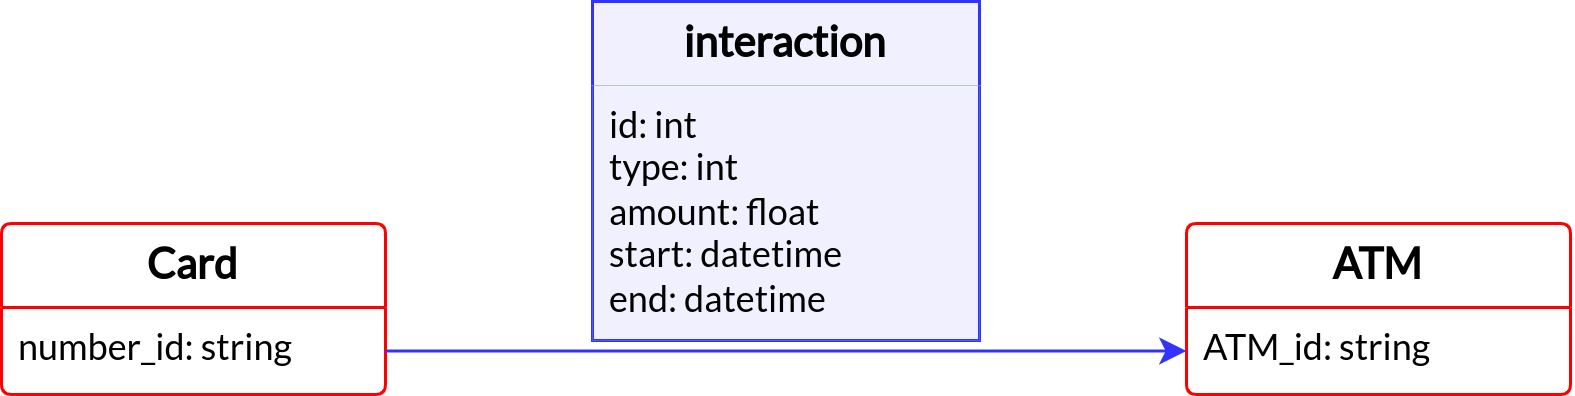
\includegraphics[scale = 0.8]{images/1-DataModel/schema-volatile.png}
    \caption{Volatile property graph model}
    \label{img:pg-volatile}
\end{figure}


As a whole, the proposed property graph data model is represented in Figure \ref{img:pg-complete}. where both the stable and volatile property subgraphs are merged to give a full view on the final property graph model.

\begin{figure}[h]
  \centering
  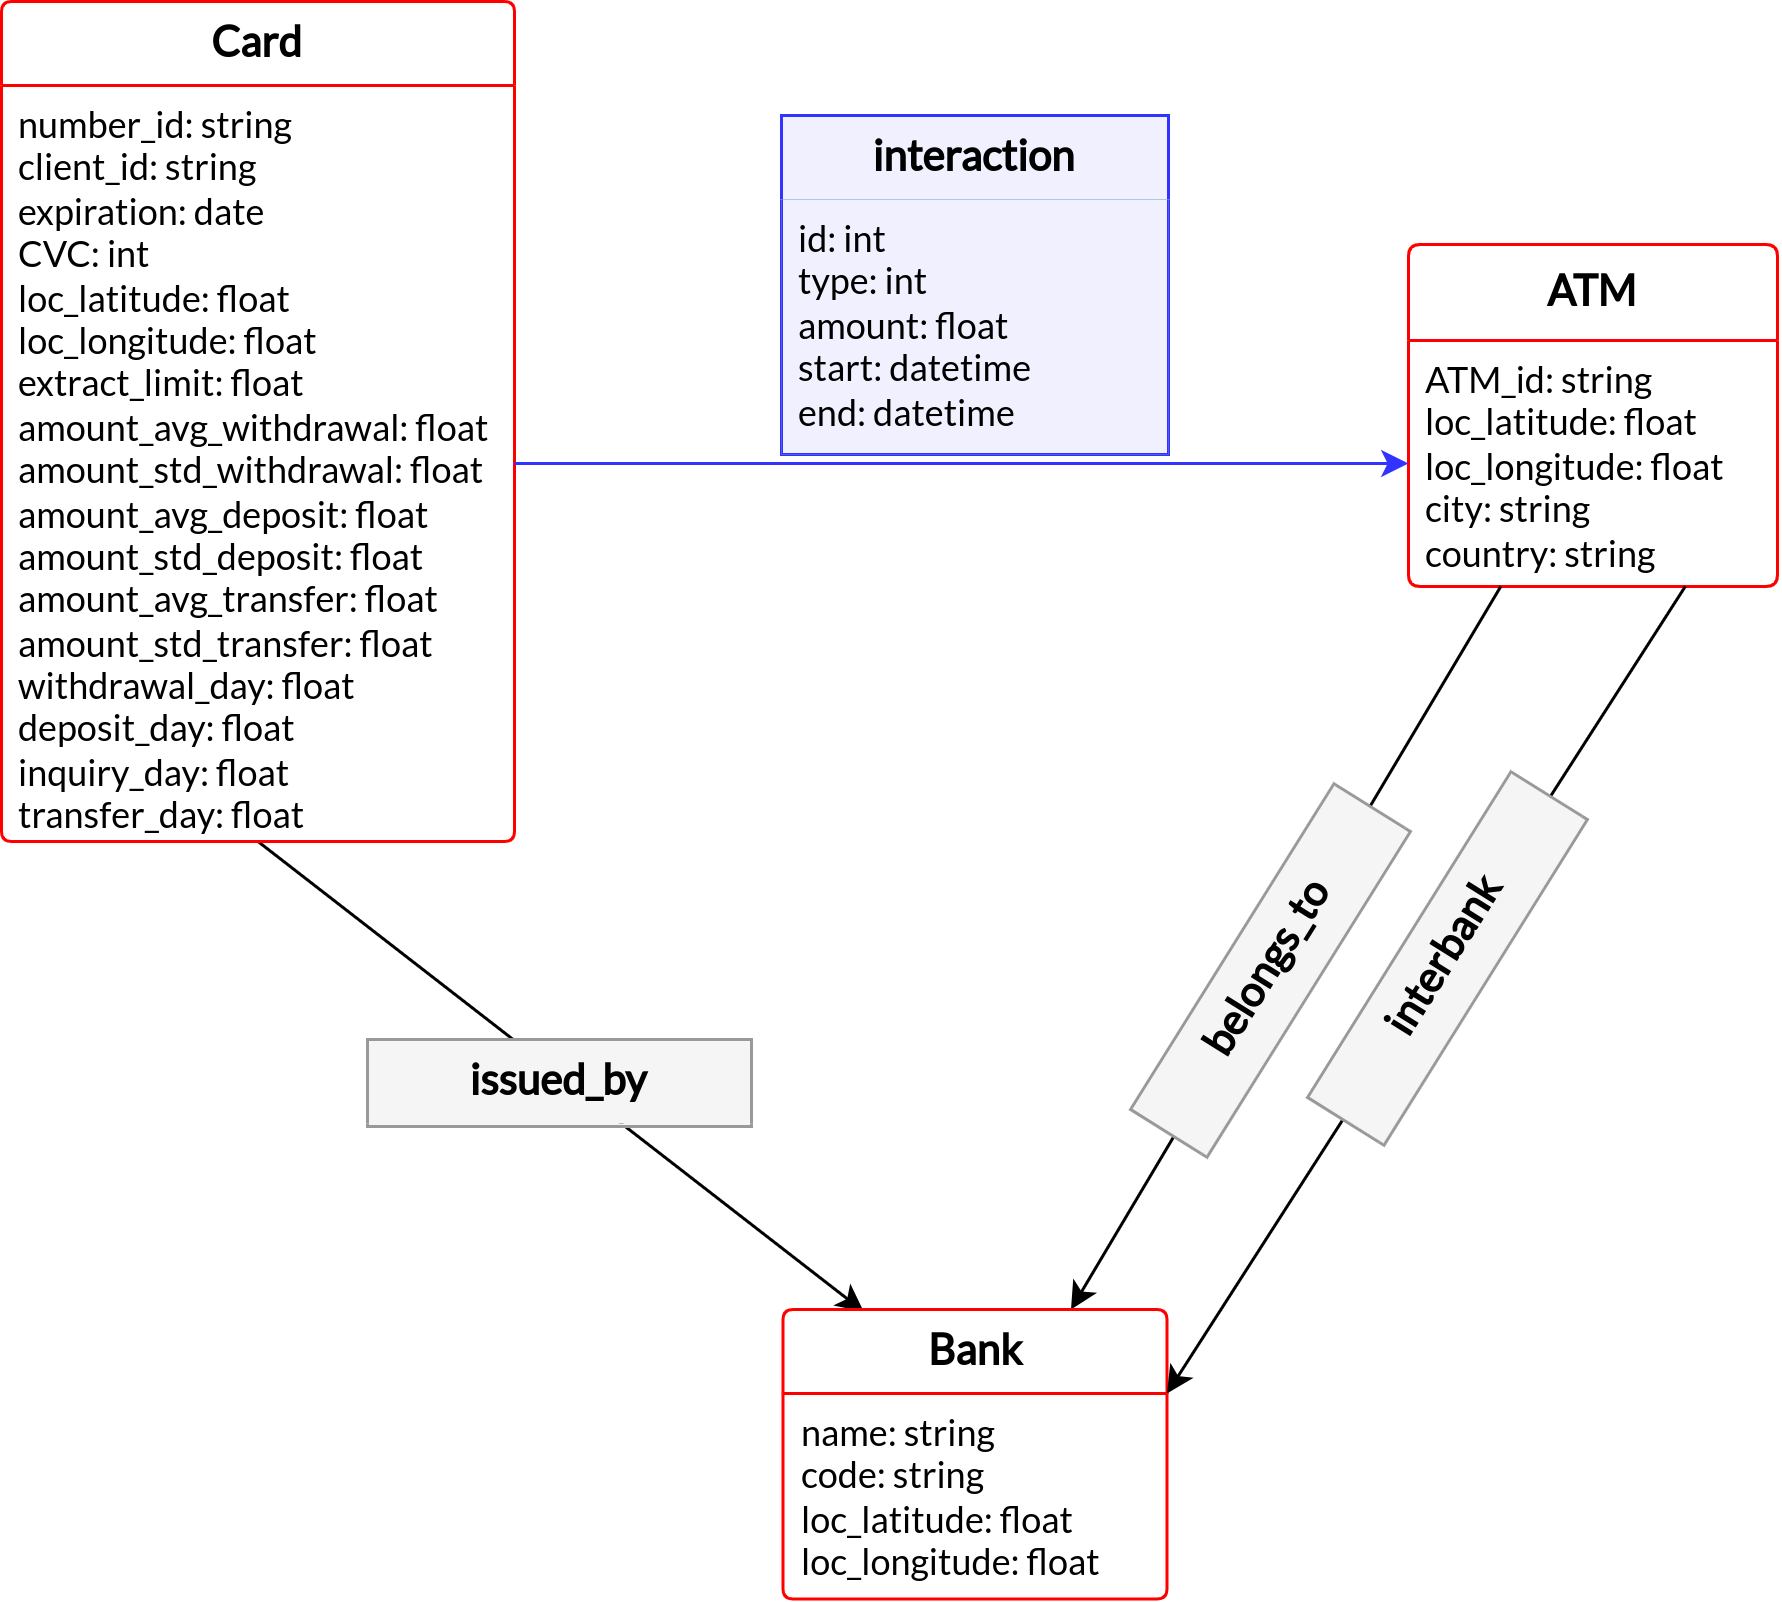
\includegraphics[scale = 0.7]{images/1-DataModel/PG-behavior-complete.png}
  \caption{Complete property graph model}
  \label{img:pg-complete}
\end{figure}

\subsection{Creation of the Synthetic Dataset}

As mentioned, given the confidential and private nature of bank data, it was not possible to find any real bank datasets. In this regard, a synthetic stable property graph bank database and a set of synthetic transactions were built based on the \emph{Wisabi Bank Dataset}\footnote{\href{https://www.kaggle.com/datasets/obinnaiheanachor/wisabi-bank-dataset}{Wisabi bank dataset on kaggle}}. The \emph{Wisabi Bank Dataset} is a fictional banking dataset that was made publicly available in the Kaggle platform. We considered it of interest as a base for the synthetic bank
database that we wanted to develop. The interest to use this bank dataset as a base was mainly because of its size: it contains 8819 different customers, 50 different ATM locations and 2143838 transactions records of the different customers during a full year (2022). Additionally, it provides good heterogenity on the different kind of transactions: withdrawals, deposits, balance inquiries and transfers. The main uses of this bank dataset are the obtention of a geographical distribution for
the locations of our generated ATMs and the construction of a card/client \emph{behavior}, which we will use for the generation of the synthetic transactions.

In particular, we divide the creation of the synthetic dataset in two. On the one hand on the creation of the stable bank database and on the other hand on the creation of the set of synthetic transactions and anomalous transactions that will conform the stream of data reaching our system.

\paragraph{Details of the \emph{Wisabi Bank Dataset\\}}
The \emph{Wisabi Bank Dataset} consists on ten CSV tables. Five of them are of transaction records of five different states of Nigeria (Federal Capital Territory, Lagos, Kano, Enugu and Rivers State) that refers to transactions of cardholders in ATMs. In particular they contain 2143838 transactions records done during the year 2022, of which 350251 are in Enugu, 159652 in Federal Capital Territory, 458764 in Kano, 755073 in Lagos and 420098 in Rivers. Then, the rest of the tables are: a customers table (`customers\_lookup`) where the data
of 8819 different cardholders is gathered, an ATM table (`atm\_location lookup`) with
information of each of the 50 different locations of the ATMs, and then three remaining
tables as complement of the previous ones (`calendar lookup`, `hour lookup` and 
`transaction\_type lookup`) 
(\href{https://app.diagrams.net/#G1eAn47YR7-zPNE5KgStkA6_IJcxZRYgX8#%7B%22pageId%22%3A%22R2lEEEUBdFMjLlhIrx00%22%7D}{tables summary}).

\subsubsection{Stable Bank Database}

To do the generation of a stable bank database we provide the Python program \texttt{bankDataGenerator.py}, in which it is needed to enter the bank properties' values, 
as well as the parameters on the number of the bank ATMs (internal and external) and Cards: \texttt{n} and \texttt{m}, respectively. 

% How to use the bankDataGenerator
\paragraph{How to use the bank data generator}

\begin{enumerate}
    \item Ensure to have the provided \texttt{wisabi} directory with the csv files from \emph{Wisabi Bank Dataset}.
    \item Run \texttt{\$> python3.10 bankDataGenerator.py} -- Run with Python3.6 version or higher -- Introduce:
    \begin{enumerate}
        \item Bank properties' values.
        \item $n = |ATM|$, internal and external.
        \item $m = |Cards|$.
    \end{enumerate}
\end{enumerate}

In what follows we give the details on the generation of the instances of our static database entities.
For simplicity and to do it in a more stepwise manner, we are going to first create all the CSV data tables for the nodes and for the relations in the corresponding format and then we will populate the Neo4j GDB with them.

\paragraph{Bank}

Since a unique bank instance is considered, the values of the properties of the bank node are manually assigned, leaving them completely customisable.
For the bank, we will generate \texttt{n} ATM and \texttt{m} Card entities. Note that apart from the generation of the ATM and Card node types we will also need to generate the relationships between the ATM and Bank entities (\texttt{belongs\_to} and \texttt{external}) and the Card and Bank entities (\texttt{issued\_by}).

\paragraph{ATM}

We generate $\texttt{n = n\_internal + n\_external}$ ATMs, where \texttt{n\_internal} is the number of internal ATMs owned by the bank and \texttt{n\_external} is the number of external ATMs that are accesible to the bank.
The generation of \texttt{n} ATMs for the bank is done following
the geographical distribution of the locations of the ATMs in the \emph{Wisabi Bank Dataset}. 
On this dataset there are 50 ATMs locations distributed along Nigerian cities. 
Note that for each of these ATMs locations, there can be more than one ATM.
However, this is not taken into account and only one ATM per location is assumed for the 
distribution.\\
\textcolor{red}{$\Rightarrow$ Put a plot of the distribution of the ATM locations}\\
This distribution of the ATMs matches the relevance of the location in terms of its population, since the number of ATM locations is larger in the most populated 
Nigerian cities (30\% of the ATM locations are in the city of Lagos, then the 20\% in Kano...). Therefore, for the generation of the location of each of the \texttt{n} ATMs, the location/city of an ATM selected uniformly at random from the \emph{Wisabi Bank Dataset} is assigned as \emph{city} and \emph{country}. Then, new random geolocation coordinates inside a bounding box of this city location are set as the \emph{loc\_latitude} and \emph{loc\_longitude} exact coordinates of the ATM. \\
Finally, as the ATM unique identifier \emph{ATM\_id} it is assigned a different code depending on the ATM internal or external category: 

\[
\emph{ATM\_id} =
\begin{cases} 
bank\_code + "-" + i & 0 \leq i < \texttt{n\_internal } \text{if internal ATM}  \\
EXT + "-" + i & 0 \leq i < \texttt{n\_external } \text{if external ATM}
\end{cases}
\]

\paragraph*{Card}

We generate a total of \texttt{m} cards that the bank manages, for each of them the assignment of the different properties is done as follows:

\begin{itemize}
\item Card and client identifiers:

\[
\begin{cases} 
number\_id = \text{c-}bank\_code\text{-}i \\
client\_id = i 
\end{cases}
0 \leq i < \texttt{m}
\]

\item \texttt{Expiration} and \texttt{CVC} properties: they are not relevant, could be empty 
  value properties indeed or a same toy value for all the cards. For completeness the  
  same values are given for all the cards: $\texttt{Expiration} = \text{2050-01-17}$, $\texttt{CVC} = 999$.

\item Client's habitual address location (\texttt{loc\_latitude}, \texttt{loc\_longitude}): two possible options were designed to define the client habitual residence address. In both 
cases they are random 
coordinates drawn from a bounding box of a location/city. The difference is on how the selection of the location/city is done:

  \begin{enumerate}
      \item Wisabi customers selection: Take the city/location of the habitual ATM of a random selected \emph{Wisabi} database customer. Note that in the \emph{Wisabi Bank Dataset} customers contain an identifier
      of their usual ATM, more in particular, the dataset is designed in such a way that customers
      only perform operations in the same ATM.
      With this approach, we maintain the geographical distribution of the \emph{Wisabi} customers.
      \item Generated ATMs selection: Take the city/location of a random ATM of the \texttt{n} generated ATMs. This method is the one utilized so far.
  \end{enumerate}

\item[$\circ$]\textbf{\emph{Behavior}}: It contains relevant attributes that will be of special interest when performing the 
generation of the synthetic transactions of each of the cards. The defined \emph{behavior}
parameters are shown in Table \ref{table:behavior-parameters}. 

\begin{table}[H]
    \centering
    \begin{tabular}{|l|l|}
        \hline
        \textbf{Behavior Property} & \textbf{Description} \\ 
        \hline
        $\mathsf{amount\_avg\_withdrawal}$ & Withdrawal amount mean\\ 
        \hline
        $\mathsf{amount\_std\_withdrawal}$ & Withdrawal amount standard deviation \\ 
        \hline
        $\mathsf{amount\_avg\_deposit}$ & Deposit amount mean \\ 
        \hline
        $\mathsf{amount\_std\_deposit}$ & Deposit amount standard deviation\\ 
        \hline
        $\mathsf{amount\_avg\_transfer}$ & Transfer amount mean \\ 
        \hline
        $\mathsf{amount\_std\_transfer}$ & Transfer amount standard deviation \\ 
        \hline
        $\mathsf{withdrawal\_day}$ & Average number of withdrawal operations per day \\ 
        \hline
        $\mathsf{deposit\_day}$ & Average number of deposit operations per day \\ 
        \hline
        $\mathsf{transfer\_day}$ & Average number of transfer operations per day \\ 
        \hline
        $\mathsf{inquiry\_day}$ & Average number of inquiry operations per day \\ 
        \hline
    \end{tabular}
    \caption{\emph{Behavior} properties}
    \label{table:behavior-properties}
\end{table}


For each card, its \emph{behavior} parameters are gathered from the transactions record of a randomly selected customer on the \emph{Wisabi Bank Dataset}, from which we can access the transactions record of $8819$ different customers for one year time interval. On it, there are four different types of operations that a customer can perform: withdrawal, deposit, balance inquiry and transaction. The parameters for the \emph{behavior} gather information about these four different types of operations. Note that all these \emph{behavior} parameters are added as additional fields of the CSV generated card instances, so, as mentioned, they can later be utilized for the generation of the synthetic
transactions.

Another possible way to assign the \emph{behavior} parameters could be the assignation
of the same behavior to all of the card instances. However, this method will provide less variability in
the generation of the synthetic transactions than the aforementioned method. 
Nevertheless, other taylored generation methods to generate different \emph{behavior} for 
each the cards could also be considered to similarly obtain this
variability.

\item \textcolor{red}{\texttt{extract\_limit}: $\texttt{amount\_avg\_withdrawal} * 5$} Other possible ways could be chosen for assigning a value to this property.
\end{itemize}

\subsubsection{Transactions Set}

The transaction set constitutes the simulated input data stream continuously arriving to the system. Each transaction represents the operation done by a client's card on a ATM of the bank network. Therefore it has the form of a \emph{interaction} edge/relation from the volatile subgraph (see \ref{section:volatile-pg}) matching one Card with one ATM from the stable bank database.

Note that, as in our definition of the input data stream of the $DP_{CQE}$, we will generate two edges per transaction -- the \emph{opening} and the \emph{closing} edge -- which both will constitute a single \emph{interaction} relation. The \emph{opening} edge (Figure \ref{img:opening-edge}) will be the indicator of the beginning of a new transaction between the matched Card and ATM, it contains the values of the properties related with the starting time \texttt{start}, the transaction \texttt{type} as well as the \texttt{id}. The \emph{closing} edge (Figure \ref{img:closing-edge}) will indicate the end of the transaction, completing the values of the rest of the properties of the \emph{interaction}: \texttt{end} and \texttt{amount}.

\begin{figure}[h]
  \centering
  \includegraphics[scale = 0.8]{images/1-DataModel/2-edges-tx-tfm.png}
  \caption{\emph{Opening} interaction edge}
  \label{img:opening-edge}
\end{figure}

\begin{figure}[h]
  \centering
  \includegraphics[scale = 0.8]{images/1-DataModel/2-edges-tx-tfm-1.png}
  \caption{\emph{Closing} interaction edge}
  \label{img:closing-edge}
\end{figure}

We divide the generation of the transaction set in two subsets: the regular transaction set and the anomalous transaction set. The regular transaction set consists of the \emph{ordinary/correct} transactions, whereas the anomalous transaction set is composed of the \emph{irregular/anomalous} transactions that are intentionally created to produce anomalous scenarios.
The main objective under this division is the ability to have the control on the exact number of anomalous ATM transactions that we generate so that we can later measure the efficiency of our system detecting them. \textcolor{gray}{as we have the exact number of anomalous transactions created to compare with, represented by size of the anomalous subset. Otherwise, if we were generating all the transactions together at the same time it would be more difficult to have the control on the amount of anomalous scenarios created, so that later, it will not be possible to measure the efficiency of our system detecting them, since we will not know their amount.}


\textcolor{blue}{To do the generation of the synthetic set of transactions we created the Python program \texttt{transactionGenerator.py}. On it we need to specify the value of the parameters needed to customise the generation of the set of transactions.}

\textcolor{red}{\rule{\linewidth}{0.5mm}}
\textcolor{red}{Notas de Fernando... $\rightarrow$ para eliminar\\}

\begin{tcolorbox}
  \begin{itemize}
    \item \textcolor{green}{$\Rightarrow$}\textbf{By card}: Generation of the transactions for each of the cards independently. \textbf{We have
    control} to avoid anomalous scenarios when selecting the ATMs and distributing the transactions along time.
    \item \textbf{In general}: Linking ATM and client composing (card,ATM) pairs, and distributing these pairs along
    time according to a certain distribution. \textbf{No control / More difficult to control the possible derived
    anomalous scenarios produced among same card pairs}.
  \end{itemize}
\end{tcolorbox}

Therefore, the generation by card option it is considered to be the best so to be able to have the control
on the possible anomalous scenarios for the generated transactions of each of the cards. Some ideas to explore:

\begin{itemize}
  \item Selection of ATMs:
  \begin{itemize}
    \item \textcolor{green}{$\Rightarrow$} Neighborhood / Closed ATM subset.
    \item Random walk. To do the selection of the sequence of ATMs for the generated transactions.
  \end{itemize}
  \item Distribution of the transactions along time:
  \begin{itemize}
    \item \textcolor{green}{$\Rightarrow$} Uniform distribution.
    \item \textcolor{blue}{$\Rightarrow$ (Consider the possibility)} Poisson process distribution.
  \end{itemize}
  \item Other options:
  \begin{itemize}
    \item Random walk for both the ATM and the transaction time selection, in the same algorithm together.
  \end{itemize}
\end{itemize}

\textcolor{red}{TODOS:
\begin{itemize}
\item Cambiar/Actualizar dibujos
\item Poner lista de params y explicar (tabla) como y qué se puede configurar
\item Poner instrucciones de como correr el generador!!!
\item Prerequisitos: csv directory has to exist - create it beforehand better
\item Output files that are generated: regular, anomalous and all csvs.
\item Anomalous generator:
\begin{itemize}
  \item NO-Overlapping assumption - Explain
  \item Any type of tx to produce the fraud -> does not matter the type for the FP1.
\end{itemize}
\end{itemize}
}

\textcolor{red}{\rule{\linewidth}{0.5mm}}

\paragraph{Regular Transaction Set\\\\}

The key idea of the transactions of this set is to avoid the creation of anomalous scenarios among them, so to have a close-to-reality simulation of a bank transaction stream flow free of all the kinds of anomalies considered. After this set is created, the transactions producing anomalous scenarios related with each specific fraud pattern will be produced.

We generate transactions for each of the generated cards on our bank network, based on each of the gathered card transaction behavior. The regular transaction data stream is generated for a customisable \texttt{NUM\_DAYS} number of days starting in a \texttt{START\_DATE}. As a summary of the procedure we first show a pseudocode of the transaction generator in Algorithm \ref{alg:regular-tx-generator}, of which later some of its parts are explained.

\begin{algorithm}[H]
  \small
  \begin{algorithmic}[1]
  \STATE $\texttt{id} \gets 0$
  \FOR{\text{card} in \text{cards}}
    \STATE $\texttt{ATM\_subset}, \overline{\texttt{ATM\_subset}} \gets \text{createATMsubset(\texttt{residence\_loc})}$
    \STATE $\texttt{t\_min\_subset} \gets \text{calculate\_t\_min\_subset(\texttt{ATM\_subset})}$
    \STATE $\texttt{num\_tx} \gets \text{decide\_num\_tx()}$
    \STATE $T \gets \text{distribute}(\texttt{num\_tx}, \texttt{t\_min\_subset})$
    \FOR{$t_i$ in $T$}
        \STATE $\texttt{ATM}_{i} \sim \texttt{ATM\_subset}$
        \STATE $\texttt{start}_{i} \gets t_i.start$
        \STATE $\texttt{end}_{i} \gets t_i.end$
        \STATE $\texttt{type}_{i} \gets \text{getType()}$
        \STATE $\texttt{amount}_{i} \gets \text{getAmount()}$
        \STATE $\texttt{id}_{i} \gets \texttt{id}; \ \texttt{id} \gets \texttt{id} + 1$
        \STATE $\text{createTransaction}(\texttt{id}_{i}, \texttt{ATM}_i, \texttt{start}_{i},\texttt{end}_{i}, \texttt{type}_{i}, \texttt{amount}_i)$
    \ENDFOR
    \STATE $\text{introduceAnomalous}(\texttt{ATM\_subset}, \overline{\texttt{ATM\_subset}})$
  \ENDFOR
  \end{algorithmic}
  \caption{Regular Transactions Generation}
  \label{alg:regular-tx-generator}
\end{algorithm}

\begin{comment}
For a card, the idea is to create a certain 
number of transactions per day, by linking the card to a certain ATM that is no farther 
than \textcolor{orange}{\texttt{max\_distance}} kms from the residence location of the 
client of the card. Also, we will limit the time distance between two consecutive 
transactions so that the final set of created transactions can not produce a potential 
fraud related with having two transactions in different ATM locations with an insufficient 
feasible time distance.
\end{comment}

\begin{enumerate}
    \item \textbf{Creation of the ATM subset} \\
    {\footnotesize \textcolor{teal}{$\texttt{ATM\_subset}, \overline{\texttt{ATM\_subset}} \gets \text{createATMsubset(\texttt{residence\_loc})}$}}
    
    Among all the ATMs of the stable bank database we create a subset of ATMs \texttt{ATM\_subset}, such that all the regular transactions generated for this card take place in (randomly selected) ATMs of this subset. 
    $\texttt{ATM\_subset} = \{\texttt{ATM}\
    |\ \texttt{distance(ATM,residence\_loc)} \\ \leq \texttt{MAX\_DISTANCE\_SUBSET\_THRESHOLD}\}$. \texttt{ATM\_subset} consists of the ATMs that are considered to be \textit{usual} for the card, considering the ATMs that are at a distance lower or equal to a customisable maximum distance threshold \texttt{MAX\_DISTANCE\_SUBSET\_THRESHOLD} to the registered residence location \texttt{residence\_loc} on the card. We also limit the size of this subset, considering only a maximum ratio of the total number of ATMs (\texttt{MAX\_SIZE\_ATM\_SUBSET\_RATIO} $\in [0,1]$), so that only a certain ratio of the closest ATMs are included on it: 
    $$|\texttt{ATM\_subset}| = \texttt{MAX\_SIZE\_ATM\_SUBSET\_RATIO} * |\texttt{ATM}|$$ 

\textcolor{red}{TODO: CAMBIAR ESTA IMAGEN}
    \begin{figure}[H]
      \centering
      \includegraphics[scale=1.1]{images/1-DataModel/tx-generation-1-named.png}
      \caption{\texttt{Neighborhood} ATM subset}
    \end{figure}

    \item \textbf{Calculate \texttt{t\_min\_subset}} \\
    {\footnotesize\textcolor{teal}{$\texttt{t\_min\_subset} \gets \text{calculate\_t\_min\_subset(\texttt{ATM\_subset})}$}}
    
    Minimum threshold time between any two consecutive transactions of the card. That is, the minimum time distance between the end of a transaction and the start of the next consecutive transaction of a card. For it, we take the time needed to traverse the maximum distance between any pair of ATMs of the \texttt{ATM\_subset}: \texttt{max\_distance\_subset} at an assumed speed that any two points can be traveled for the case of ordinary scenarios: \texttt{REGULAR\_SPEED}.
    $$\texttt{t\_min\_subset} = \frac{\texttt{max\_distance\_subset}}{\texttt{REGULAR\_SPEED}}$$

    \item \textbf{Decide the number of transactions \texttt{num\_tx}}\\
    {\footnotesize \textcolor{teal}{$\texttt{num\_tx} \gets \text{decide\_num\_tx()}$}}
    
    
    Based on the behavior of the card, we decide the number of transactions (\texttt{num\_tx}) to generate for the card for the selected number of days \texttt{NUM\_DAYS} as:

    $$\texttt{num\_tx} \sim \text{Poisson}(\lambda = \texttt{ops\_day} * \texttt{NUM\_DAYS})$$ where \texttt{ops\_day} is the sum of the average number of all the kinds of operations per day of the particular card: 
    $$\texttt{ops\_day} = \texttt{withdrawal\_day} + \texttt{ deposit\_day} + \texttt{ inquiry\_day} + \texttt{ transfer\_day}$$


    \item \textbf{Decide on the type of transaction}\\
    {\footnotesize \textcolor{teal}{$\texttt{type}_{i} \gets \text{getType()}$}}

    
    For each of the \texttt{num\_tx} transactions, the transaction \texttt{type} is decided randomly assigning a transaction \texttt{type} given a probability distribution constructed from the card behavior:
    
    $$
    \begin{cases}
      P(\texttt{type} =  \texttt{withdrawal}) = \frac{\texttt{withdrawal\_day}}{\texttt{ops\_day}} \\[8pt]
      P(\texttt{type} =  \texttt{deposit}) = \frac{\texttt{deposit\_day}}{\texttt{ops\_day}} \\[8pt]
      P(\texttt{type} = \texttt{inquiry}) = \frac{\texttt{inquiry\_day}}{\texttt{ops\_day}} \\[8pt]
      P(\texttt{type} =  \texttt{transfer}) = \frac{\texttt{transfer\_day}}{\texttt{ops\_day}} 
    \end{cases}
    $$

    \item \textbf{Distribution of the \texttt{num\_tx} transaction times} \\
     {\footnotesize \textcolor{teal}{$T \gets \text{distribute}(\texttt{num\_tx}, \texttt{t\_min\_subset})$}}
    
    Along the selected time interval starting in \texttt{START\_DATE} and finishing \texttt{NUM\_DAYS} days after we do a random uniform distribution of the \texttt{num\_tx} transaction times. $T$ contains the list of all the the \texttt{start} and \texttt{end} times tuples for each of the \texttt{num\_tx} transactions, with the constraint that, for each transaction $i$, the next one $i+1$ is at a minimum time distance of \texttt{t\_min\_subset}. Specifically, the transaction times are generated guaranteeing:

    $$i.\texttt{end} + \texttt{t\_min\_subset} < (i+1).\texttt{start} \ \forall i \in [1,\texttt{num\_tx})$$

    The \texttt{end} time of a transaction is assigned a shifted time difference with respect to the \texttt{start} time. In particular:

    $$
    \texttt{end} = \texttt{start} + \texttt{time\_difference}
    $$

    where:

    $$\texttt{time\_difference} \sim \mathcal{N}(\texttt{MEAN\_DURATION},\,\texttt{STD\_DURATION})$$ with the corrections:

    $$
    \texttt{time\_difference} =
    \begin{cases} 
        \texttt{MEAN\_DURATION} & \text{if } \texttt{time\_difference} < 0 \\
        \texttt{MAX\_DURATION} & \text{if } \texttt{time\_difference} > \texttt{MAX\_DURATION} \\
        \texttt{time\_difference} & \text{otherwise}
    \end{cases}
    $$

\textcolor{red}{TODO: PONER UN DIBUJITO!, explicar lo del checking de los fitting holes? --> yo creo que esto ya no es necesario... demasiado detalle}


  \item Assign a transaction \texttt{amount}\\
  {\footnotesize \textcolor{teal}{$\texttt{amount}_{i} \gets \text{getAmount()}$}}
  
  Amount is assigned depending on the \texttt{type} based on card behavior:
    
  $$
  \begin{cases}
    \mathcal{N}(\texttt{amount\_avg\_withdrawal},\, \texttt{amount\_std\_withdrawal}) & \text{if } \texttt{type} = \texttt{withdrawal} \\[10pt]
    
    \mathcal{N}(\texttt{amount\_avg\_deposit},\, \texttt{amount\_std\_deposit}) & \text{if } \texttt{type} = \texttt{deposit} \\[10pt]

    0 & \text{if } \texttt{type} = \texttt{inquiry} \\[10pt]
    
    \mathcal{N}(\texttt{amount\_avg\_deposit},\, \texttt{amount\_std\_transfer}) & \text{if } \texttt{type} = \texttt{transfer}
  \end{cases}
  $$

  $$
  \text{If } \texttt{amount} < 0, \text{ then re-draw from } U(0, 2 \cdot \texttt{amount\_avg\_type}).
  $$

  with \texttt{amount\_avg\_type} as \texttt{amount\_avg\_withdrawal}, \texttt{amount\_avg\_deposit} or \texttt{amount\_avg\_deposit} depending on the respective transaction \texttt{type}.

\end{enumerate}

\paragraph{Anomalous Transaction Set\\\\}

After the generation of regular transactions we perform an injection of transactions to produce anomalous scenarios. The injection is taylored depending on the specific kind of 
anomalous scenarios that we want to produce. In what follows we explain the injection process depending on each of the types of frauds that we have considered.

\paragraph{Fraud Pattern I}

To produce anomalous scenarios related to this type of fraud, we produce the injection
of transactions that will produce the satisfaction of this fraud pattern. In other words,
we inject transactions that violate the minimum \emph{time-distance} constraint between transactions performed with the same card. Therefore, as we can see in Figure \ref{img:anomalous-type-1}, if we consider a set of regular transacions for a certain card, where $y_1$ and $y_2$ are regular consecutive transactions, we will introduce an anomalous transaction $a_{12}$ such that: 

$$(y_1.\texttt{ATM\_id} \ne a_{12}.\texttt{ATM\_id}) \land (a_{12}.\texttt{start} - 
y_1.\texttt{end} < T_{min}(y_1.\texttt{ATM\_loc}, a_{12}.\texttt{ATM\_loc}))$$

where \texttt{ATM\_loc} is the tuple of coordinates (loc\_latitude,loc\_longitude) of the corresponding ATM. This injection will produce an anomalous scenario of this kind of fraud with at least the $y_1$ previous transaction. Note that, it could possibly trigger more anomalous fraud scenarios with the subsequent transactions ($y_2$ and on...).

\begin{figure}[H]
    \centering
    \includegraphics[width=\textwidth]{images/1-DataModel/tx-generation.png}
    \caption{Creation of anomalous scenario - type I}
    \label{img:anomalous-type-1}
\end{figure}

Some assumptions related with the generation of anomalous transactions for this kind of fraud pattern are:
\begin{itemize}
  \item \textbf{Overlapping of transactions is not possible}:
  Appart from guaranteeing that this injection causes at least one anomalous scenario, we also respect the additional constraint of ensuring that the anomalous transaction injected does not cause overlapping with any of the transactions, in particular neither with the previous nor the next one. \textcolor{orange}{This constraint is added based on the assumption that the bank itself does not allow to open a transaction whenever another one is still open.} Therefore considering that $a_{12}$ is the anomalous injected transaction in between the regular consecutive transactions $y_1$ and $y_2$, when generating $a_{12}$ we guarantee that:
  $$
  \begin{cases}
    a_{12}.\texttt{start} > y_{1}.\texttt{end} \\
    a_{12}.\texttt{end} < y_{2}.\texttt{start}
  \end{cases}
  $$
  \item \textbf{There are no two consecutive anomalous transactions}: For simplicity in our practical purposes, we do the generation of anomalous transactions for this kind of fraud pattern assuming that an anomalous transaction can only be in between two regular consecutive transactions, so that we do not consider the case of the injection of two or more consecutive anomalous transactions for this kind of fraud. See Figure \ref{img:anomalous-type-1-insertion-points}.
  \begin{figure}[H]
    \centering
    \includegraphics[width=\textwidth]{images/1-DataModel/tx-generation-anomalous-1.png}
    \caption{Considered possible injection points of anomalous transactions of fraud type I}
    \label{img:anomalous-type-1-insertion-points}
  \end{figure}  
\end{itemize}

We generate $\texttt{ANOMALOUS\_RATIO\_1} * \texttt{num\_tx}$ anomalous transactions for each of the cards related with the fraud pattern I, where $\texttt{ANOMALOUS\_RATIO\_1} \in [0,1]$ defines the ratio of anomalous transactions of this kind over the total number of regular transactions \texttt{num\_tx} for each of the cards. In Algorithm \ref{alg:anomalous-tx-generator-1} we describe at a high level the process of the generation of anomalous transactions for this kind of fraud pattern. 


\textcolor{red}{Preconditions:
\begin{itemize}
  \item ATMsubset, and the compl. are given by param, from the tx regular generator
\end{itemize}
}

\begin{algorithm}[H]
  \small
  $\textbf{introduceAnomalous}(\texttt{ATM\_subset}, \overline{\texttt{ATM\_subset}})$
  \begin{algorithmic}[1]
  \STATE $\texttt{num\_anomalous} \gets \texttt{num\_tx} * \texttt{ANOMALOUS\_RATIO\_1}$
  \STATE $i \gets 0$
  \WHILE{$i < \texttt{num\_anomalous}$}
      \STATE $\texttt{ATM}_{i} \sim \overline{\texttt{ATM\_subset}}$
      \STATE $prev_i, next_i \gets \text{randomUniquePosition(\texttt{num\_tx})}$
      \STATE $t_i \gets \text{getTime}(prev_i, next_i)$
      \STATE $\texttt{start}_{i} \gets t_i.start$
      \STATE $\texttt{end}_{i} \gets t_i.end$
      \STATE $\texttt{type}_{i} \gets \texttt{getRandomType()}$
      \STATE $\texttt{amount}_{i} \gets \texttt{getAmount()}$
      \STATE $\texttt{id}_{i} \gets \texttt{id}; \ \texttt{id} \gets \texttt{id} + 1$
      \STATE $\texttt{createTransaction}(\texttt{id}_{i}, \texttt{ATM}_i, \texttt{start}_{i},\texttt{end}_{i}, \texttt{type}_{i}, \texttt{amount}_i)$
      \STATE $i \gets i + 1$
  \ENDWHILE
  \end{algorithmic}
  \caption{Introduction of Anomalous Transactions for Fraud Pattern I}
  \label{alg:anomalous-tx-generator-1}
\end{algorithm}


\begin{enumerate}
  \item \textbf{Assignment of ATMs not belonging to the \texttt{ATM\_subset}}: the anomalous transactions are linked to ATMs that are part of the complementary of the \texttt{ATM\_subset}.
  \item \textbf{Each anomalous transaction has a unique insertion position}: As described previously, we do not allow the case of two or more consecutive anomalous transactions injection. Each anomalous transaction occupies a unique position among all the possible injection positions defined by the set of regular transactions generated for the card. As it can be seen on Figure \ref{img:anomalous-type-1-insertion-points}, considering that we have three regular transactions, we will consider three unique possible insertion points for the anomalous transactions. The procedure of assigning a unique insertion position for each anomalous transaction to be generated is achieved with the function \text{randomUniquePosition(\texttt{num\_tx})}, that given the number of regular transactions of the card \texttt{num\_tx} returns the previous and the next regular transaction to the assigned unique position.
  \item \textbf{Assign transaction times such that respecting the needed time constraints}: in particular there are two time constraints to be satisfied:
  \begin{itemize}
    \item Production of fraud pattern with prev\_i
    \item No overlapping with prev\_i nor with next\_i
  \end{itemize}
  This is summarized in the pseudocode as the procedure getTime(prev\_i, next\_i), which returns $t_i$, as the tuple of (\texttt{start},\texttt{end}) times.
  \item \textbf{Random transaction type}
  \item \textbf{Arbitrary amount}
 
\end{enumerate}


\begin{comment}
\subsubsection{ATM closed subset + Poisson Process}

\begin{tcolorbox}
  \begin{itemize}
    \item[$\rightarrow$] \textbf{ATM selection}: Closed ATM subset.
    \item[$\rightarrow$] \textbf{Time distribution}: Poisson process distribution of $num\_tx$ 
    transactions for each of the cards.
  \end{itemize}
\end{tcolorbox}

Generate $\texttt{num\_tx}$ transactions for a selected period of time $\texttt{t}$.
Distribution following a Poisson process distribution along $[0,t]$.
\begin{itemize}
    \item[$\bullet$] $\lambda=\texttt{avg\_tx}$ on a day for the client if $\texttt{t = 24h}$. Otherwise, 
    decide a specific $\lambda$ for the considered $\texttt{t}$.
    \item[$\bullet$] Inter-arrival times $X_1, X_2, \cdots$ are distributed following an exponential distribution:
    $X_i \sim \text{Exp}(\lambda)$. They represent the time elapsed between two of these events, e.g. $X_2$ represents the time elapsed between the first and the second arrival. Note that in this case, since we need to respect the minimum required time between two consecutive 
    transactions ($t_{min}$) so to avoid introducing anomalous undesired scenarios, we have to impose
    that: $X_i \geq \Delta_{i-1} + t_{min}, \forall X_i$, where:

    \begin{itemize}
      \item[$\circ$] $X_{i}$: time elapsed between the $i$-$1$ and $i$-th transaction.
      \item[$\circ$] $\Delta_{i-1}$: time duration of the $i$-$1$ transaction. This duration will 
      be upper bounded by $\Delta_{max}$, which will be considered the maximum possible duration of a transaction.
      \item[$\circ$] $t_{min}$: minimum calculated time distance between any 2 consecutive transactions of the client.
  \end{itemize}

    With these interarrival times, we obtain the arrival times $T_i$. Note that they are not independent, in particular:
    $T_1 \leq T_2 \leq T_3 \cdots$.

    Therefore, to generate the Poisson process with rate $\lambda$:
    \begin{enumerate}
      \item Generate i.i.d. random variables $X_1, X_2, \cdots$ where $X_i \sim \text{Exp}(\lambda)$.
      \item Obtain the arrival times as:
        \begin{itemize}
          \item $T_1 = X_1$
          \item $T_2 = X_1 + X_2$
          \item $T_3 = X_1 + X_2 + X_3$
          \item $\cdots$
        \end{itemize}
    \end{enumerate}

    Note that, having imposed the previous we will have that:
    \begin{equation}
      \begin{cases}
        T_i = T_{i-1} + X_i \\
        X_i \geq \Delta_{max} + t_{min}
      \end{cases}\forall X_i \
    \end{equation}

    which implies that:
    
    \begin{equation}
      T_i \geq T_{i-1} + \Delta_{max} + t_{min}, \forall X_i
    \end{equation}
    
\end{itemize}
\begin{figure}[H]
    \centering
    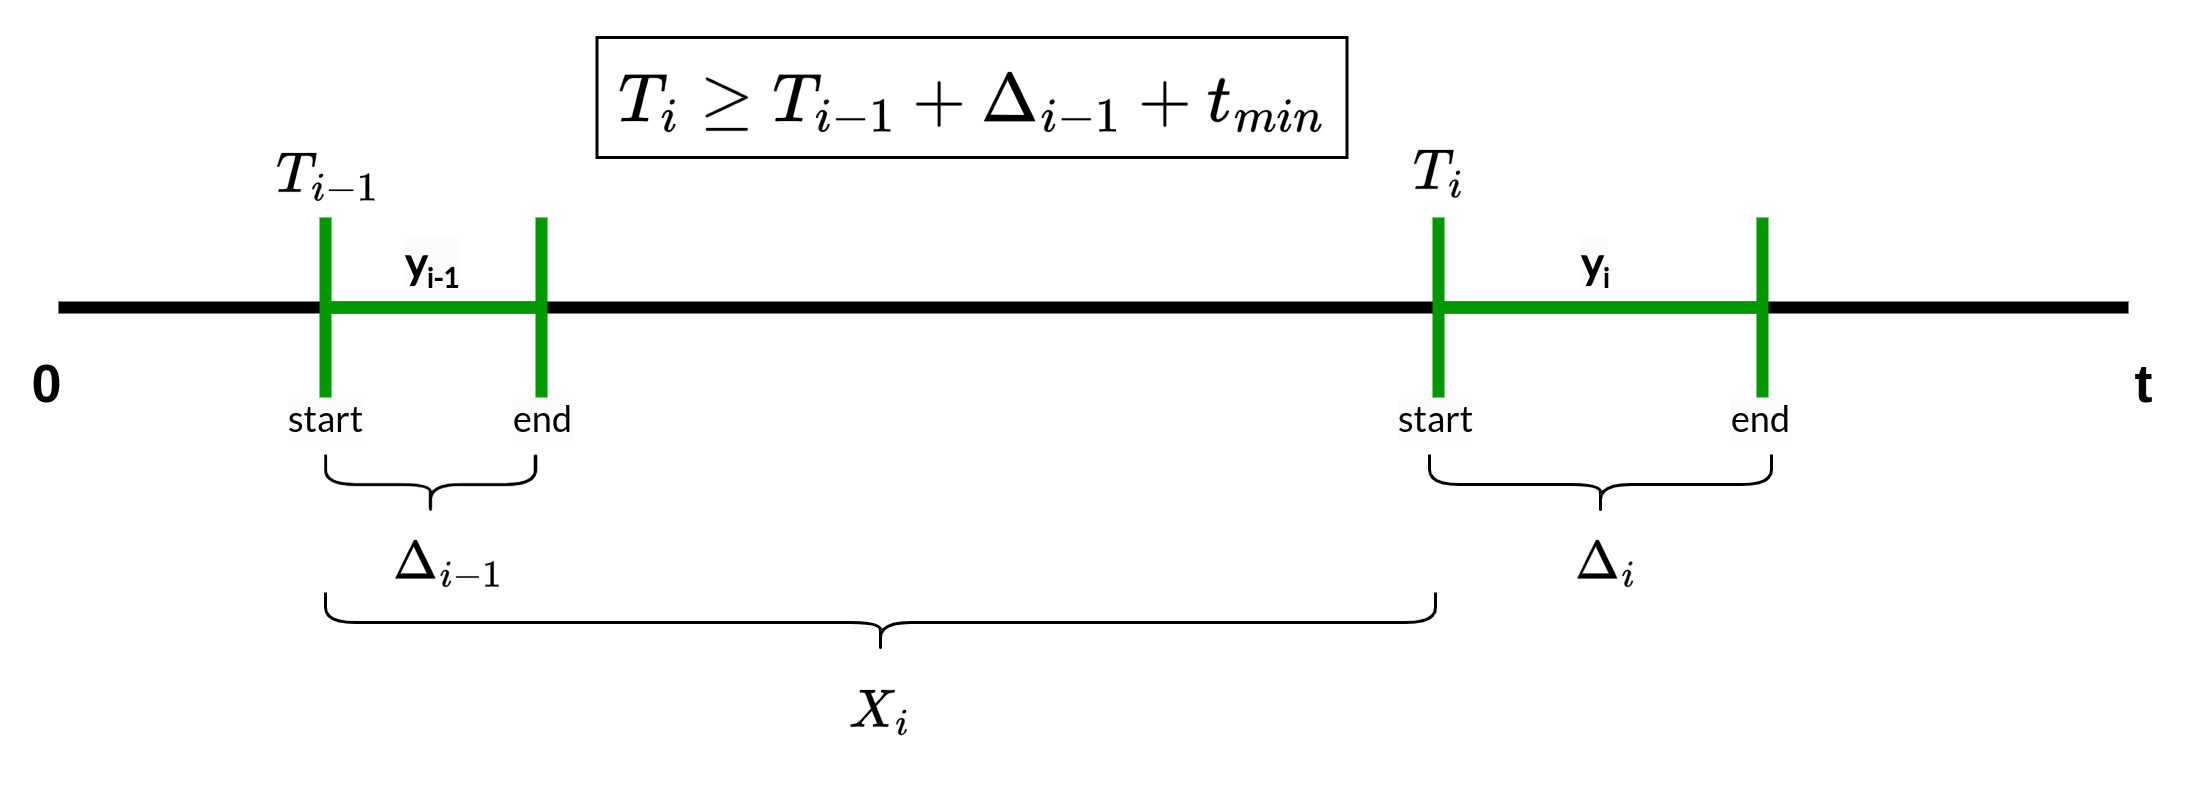
\includegraphics[scale=0.55]{images/tx-generation-dist-corrected.png}
    \caption{Schema of the interarrival and arrival event times on the poisson process.}
\end{figure}


References:

\begin{itemize}
  \item \href{https://www.probabilitycourse.com/chapter11/11_1_2_basic_concepts_of_the_poisson_process.php}{Poisson process modeling - Theoric description}
  \item \href{https://www.probabilitycourse.com/chapter14/Chapter_14.pdf}{Poisson process modeling - Python implementation}
  \item \href{https://timeseriesreasoning.com/contents/poisson-process/}{Less formal explanation with Python code}
  \item \href{https://www.math.wsu.edu/faculty/genz/416/lect/l05-45.pdf}{More theory}
  \item \href{https://en.wikipedia.org/wiki/Poisson_point_process}{Wikipedia entry}
\end{itemize}

\subsubsection{Random Walk / Markov Chain}

Idea is to model the sequence of transactions for each of the clients as a markov chain through the
network of ATMs. The network is a fully-connected graph with ATMs as nodes and edges are
weighted with the distance between each pair of ATMs as weights.

The idea is to obtain the sequence of transactions for each client as a markov chain, in which,
for each step a transaction is generated in that specific ATM node, at a certain datetime 
respecting the constraint of the minimum time distance with the previous transaction, so 
that no undesired anomalous fraud scenarios are produced. \\ 

Some considerations:
\begin{itemize}
  \item Initially, we will compute the transition matrix obtaining all the respective 
  transition probabilities. The probability of transition to another ATM-node will be 
  inversely proportional to the distance to the considered ATM-node.
  \item Transition matrix $P_t$: containing, for each state, the probability of transitioning
  between states. For example, the entry $i,j$: $(P_t)_{i,j} = \mathcal{P}(X_{t+1} = j | X_t = i)$
  contains the probability of transitioning to state $j$ when being in state $i$. 
  Note that since we assume a complete graph, and also the posibility to transition 
  to the same state, all entries of this matrix will be distinct to 0: $(P_t)_{i,j} \neq 0 \  
  \forall i,j$.
  \item Finally, once $P_t$ is computed, we perform the simulation to obtain the sequence of
  transactions for the specific card/client.
\end{itemize}

References:

\begin{itemize}
\item Markov Chains
\begin{itemize}
  \item \href{https://brilliant.org/wiki/markov-chains/}{MC - Theory}
  \item \href{https://www.columbia.edu/~ks20/4703-Sigman/4703-07-Notes-MC.pdf}{Simulation of Markov Chains - Theory}
  \item \href{https://stephens999.github.io/fiveMinuteStats/simulating_discrete_chains_1.html}{MC - Implementation example}
  \item \href{https://www.youtube.com/watch?v=G7FIQ9fXl6U}{MC - Implementation video example}
\end{itemize}
\item Random Walks
\begin{itemize}
  \item Theory:
  \begin{itemize}
    \item \href{https://ieeexplore.ieee.org/abstract/document/8911513?casa_token=vznpjKL5HG0AAAAA:hNzLCxAHBk75zCDUHsswB7ImAKgilzZcOBzxaXWz_G6U8Vy-ogbei40MoZ49M-Em5tTii0Q}{RWs: A Review of Algorithms and Applications}
    \item \href{https://www.lirmm.fr/~sau/JCALM/Josep.pdf}{RWs on Graphs}
    \item \href{https://www.fi.muni.cz/usr/gruska/random18/random1808.pdf}{RW - More theory}
  \end{itemize}
  \item Implementation examples:
  \begin{itemize}
    \item \href{https://tleise.people.amherst.edu/Math365Spring2016/RmarkdownFiles/WalkOnGraph.html}{Simple RW on a Graph - Implementation example}
    \item \href{https://graphstream-project.org/doc/Algorithms/Random-walks-on-graphs/}{A RW on a graph - Implementation}
    \item \href{https://es.mathworks.com/help/econ/simulate-random-walks-through-markov-chain.html}{Simulate Random Walks Through Markov Chain - Matlab Implementation example}
  \end{itemize}
\end{itemize}
\end{itemize}
\end{comment}


\subsection{Population of the Graph Database}

% TODO: 
% 0. Description - Neo4j, what it is, why chosen...
% 1. Creation
% 2. Population

\subsubsection{Neo4j graph database creation}
% Neo4j Desktop y version - instalación y detalles. Cómo conectarse...
% TODO: Explain how to install / connect... all the details that are in the neo4.md file
\textcolor{red}{$\rightarrow$ TODO: 0. Describe on how to set up the database}
\textcolor{red}{$\rightarrow$ TODO: Explanation of the versions of both Neo4j instances used - local and UPC VM cluster.}\\

Prior to the population of the Neo4j graph database, a Neo4j graph database instance needs to be
created. This was done both locally and in a \textcolor{red}{Virtual Machine of the UPC cluster}.

Version: Neo4j 5.21.0 Community edition. 
\begin{itemize}
    \item Accessing it: by default it runs on localhost port 7474: \texttt{http://localhost:7474}.
    Start the neo4j service locally by: \texttt{sudo systemctl start neo4j}\\
    It can be also be accessed by the internal utility \texttt{cypher-shell}. Username: \texttt{neo4j} and password: \texttt{bisaurin}.
\end{itemize}

\subsubsection{Neo4j graph database population - CSV to PG}
\begin{comment}
    - Creación de la GDB - de CSV a Neo4j PG: 
    - Poner primero los comandos cypher por separado, con las constraints de uniqueness
    y luego lo de poblar. Luego ya referir a que todo ello se tiene en un único script que 
    permite la ejecución directa (en lugar de paso a paso) en golang.
    - Incluir detalles específicos de cada CSV...
\end{comment}

Once we created the Neo4j graph database instance and all the CSV data files representing all the nodes and relations, we populate the Property Graph instance in Neo4j. Before performing the population of the GDB, we create uniqueness constraints on the properties of the nodes that we use as our \emph{de facto} IDs for the ATM and Card IDs: \texttt{ATM\_id} and \texttt{number\_id}, respectively. The reason to do this is to avoid having duplicated nodes of these types with the same ID in the database. Therefore, as an example, when adding a new ATM node that has the same \texttt{ATM\_id} as another ATM already existing in the database, we are aware of this and we do not let this insertion to happen. ID uniqueness constraints are created with the following cypher directives:

\begin{center}
\lstset{style=cypherStyle}
\begin{lstlisting}[caption={Uniqueness ID constraints}]
            CREATE CONSTRAINT ATM_id IF NOT EXISTS
            FOR (a:ATM) REQUIRE a.ATM_id IS UNIQUE
    
            CREATE CONSTRAINT number_id IF NOT EXISTS
            FOR (c:Card) REQUIRE c.number_id IS UNIQUE
    
            CREATE CONSTRAINT code IF NOT EXISTS
            FOR (b:Bank) REQUIRE b.code IS UNIQUE
\end{lstlisting}
\end{center}

Once we created the Neo4j graph database instance and all the CSV data files representing all the nodes and relations, we populate the Property Graph instance in Neo4j. For this, we propose two different methods. The first does it by directly importing the CSV files using the Cypher's \texttt{LOAD CSV} command, while the second method does it by parsing the CSV data and running the creation of the nodes and relationships using Cypher. Both methods can be found and employed using the \texttt{populatemodule} golang module.
In this module we can find the two subdirectories where each of the methods can be run. In detail, the module tree structure is depicted in Figure \ref{fig:populatemodule}. On it, the \texttt{cmd} subdirectory contains the scripts to run each of the populating methods: the first method script on \texttt{csvimport} and the second on the \texttt{cypherimport}, while the \texttt{internal} subdirectory is a library of the files with the specific functions used by these methods.

\begin{figure}[h]
\centering
\begin{forest}
  for tree={
      font=\ttfamily,              % Typewriter font for file names
      grow'=0,                      % Tree direction (left-to-right)
      child anchor=west,            % Children alignment
      parent anchor=east,           % Parent alignment
      anchor=west,                  % Tree alignment
      calign=first,                 % Aligns with the first child
      edge path={
          \noexpand\path [draw, thick, \forestoption{edge}] (!u.parent anchor) -- +(-1pt,0) |- (.child anchor)\forestoption{edge label};
      },
      inner sep=4pt,
      l=10pt,                       % Level distance
      s sep=5pt                     % Sibling distance
  }
  [populatemodule
      [cmd
        [csvimport
            [main.go]
            [.env]
        ]
        [cypherimport
            [main.go]
            [.env]
        ]
      ]
      [internal
          [common
              [common.go]
          ]
          [populate
              [populate.go]
          ]
      ]
  ]
\end{forest}
\caption{\texttt{populatemodule} file structure}
\label{fig:populatemodule}
\end{figure}

% How to run it - .env file
% Description of each of the methods


Prior to run any of these methods we need to first set up correctly the \texttt{.env} file located inside the desired method directory, where we have to define the corresponding Neo4j URI, username and password to access the Neo4j graph database instance.

\begin{itemize}
\item{\textbf{Method 1: Cypher's \texttt{LOAD CSV}}\\}
The Cypher's \texttt{LOAD CSV} clause allows to load CSV into Neo4j, creating the nodes and relations expressed on the CSV files (see \href{https://neo4j.com/docs/cypher-manual/5/clauses/load-csv/}{\textit{load-csv cypher manual}}). 
To use it simply follow these steps:
\begin{enumerate}
    \item Place all the CSVs (\texttt{atm.csv}, \texttt{bank.csv}, \texttt{card.csv}, \texttt{atm-bank-internal.csv}, \texttt{atm-bank-external.csv} 
    and \texttt{card-bank.csv}) under the \texttt{/var/lib/neo4j/import} directory
    of the machine containing the Neo4j graph database instance.
    \item Run \texttt{\$> go run populatemodule/cmd/csvimport/main.go}
\end{enumerate}

\paragraph{Process description:}

Then the different CSV files containing all the data tables of our data set, were loaded into the GDB with the following cypher directives.

% TODO: Esto es en mi local. Se recomienda por razones de seguridad... Sin embargo se puede configurar para que no sea
% así. - En el cluster veremos. De momento no pongo nada de esto!
% First, the CSV files were needed to be placed under the \texttt{/var/lib/neo4j/import} directory.

\paragraph{ATM (atm.csv)}

\begin{center}
\lstset{style=cypherStyle}
\begin{lstlisting}[caption={atm.csv}]
    LOAD CSV WITH HEADERS FROM 'file:///csv/atm.csv' AS row
    MERGE (a:ATM {
        ATM_id: row.ATM_id,
        loc_latitude: toFloat(row.loc_latitude),
        loc_longitude: toFloat(row.loc_longitude),
        city: row.city,
        country: row.country
    });
\end{lstlisting}
\end{center}

Some remarks:
\begin{itemize}
    \item \texttt{ATM} is the node label, the rest are the properties of this kind of node.
    \item Latitude and longitude are stored as float values; note that they could also be stored
    as cypher \textit{Point} data type. However for the moment it is left like this. In the future
    it could be converted when querying or directly be set as cypher point data type as property.
\end{itemize}

\paragraph{Bank (bank.csv)}

\begin{center}
\lstset{style=cypherStyle}
\begin{lstlisting}[caption={bank.csv}]
    LOAD CSV WITH HEADERS FROM 'file:///csv/bank.csv' AS row
    MERGE (b:Bank {
        name: row.name, 
        code: row.code, 
        loc_latitude: toFloat(row.loc_latitude), 
        loc_longitude: toFloat(row.loc_longitude)
    });
\end{lstlisting}
\end{center}

Note that the \texttt{code} is stored as a string and not as an integer, since to make it more clear it 
was already generated as a string code name.

\paragraph{ATM-Bank relationships (atm-bank-internal.csv and atm-bank-external.csv)}

\begin{center}
\lstset{style=cypherStyle}
\begin{lstlisting}[caption={atm-bank-internal.csv}]
    LOAD CSV WITH HEADERS FROM 'file:///csv/atm-bank-internal.csv' AS row
    MATCH (a:ATM {ATM_id: row.ATM_id})
    MATCH (b:Bank {code: row.code})
    MERGE (a)-[r:BELONGS_TO]->(b);
\end{lstlisting}
\end{center}

\begin{center}
\lstset{style=cypherStyle}
\begin{lstlisting}[caption={atm-bank-external.csv}]
    LOAD CSV WITH HEADERS FROM 'file:///csv/atm-bank-external.csv' AS row
    MATCH (a:ATM {ATM_id: row.ATM_id})
    MATCH (b:Bank {code: row.code})
    MERGE (a)-[r:INTERBANK]->(b);
\end{lstlisting}
\end{center}

\paragraph{Card (card.csv)}

\begin{center}
\lstset{style=cypherStyle}
\begin{lstlisting}[caption={card.csv}]
    LOAD CSV WITH HEADERS FROM 'file:///csv/card.csv' AS row
	MERGE (c:Card {
		number_id: row.number_id, 
		client_id: row.client_id, 
		expiration: date(row.expiration), 
		CVC: toInteger(row.CVC), 
		extract_limit: toFloat(row.extract_limit), 
		loc_latitude: toFloat(row.loc_latitude), 
		loc_longitude: toFloat(row.loc_longitude),
		amount_avg_withdrawal: toFloat(row.amount_avg_withdrawal),
		amount_std_withdrawal: toFloat(row.amount_std_withdrawal),
		withdrawal_day: toFloat(row.withdrawal_day),
		amount_avg_deposit: toFloat(row.amount_avg_deposit),
		amount_std_deposit: toFloat(row.amount_std_deposit),
		deposit_day: toFloat(row.deposit_day),
		inquiry_day: toFloat(row.inquiry_day),
		amount_avg_transfer: toFloat(row.amount_avg_transfer),
		amount_std_transfer: toFloat(row.amount_std_transfer),
		transfer_day: toFloat(row.transfer_day)
		});
\end{lstlisting}
\end{center}

Notes:
\begin{itemize}
    \item We include the fields that were generated to define the behavior of the card. They are also used for the generation of the transactions.
    \item \texttt{expiration}: set as \textit{date} data type.
\end{itemize}

\paragraph{Card-Bank relationships (card-bank.csv)}

\begin{center}
\lstset{style=cypherStyle}
\begin{lstlisting}[caption={card-bank.csv}]
    LOAD CSV WITH HEADERS FROM 'file:///csv/card-bank.csv' AS row
    MATCH (c:Card {number_id: row.number_id})
    MATCH (b:Bank {code: row.code})
    MERGE (c)-[r:ISSUED_BY]->(b);
\end{lstlisting}
\end{center}

%\subsubsection*{Dataset extensions}

\begin{comment}
- Interesting reference for coordinates and distances in cypher - https://lyonwj.com/blog/spatial-cypher-cheat-sheet 
- Transactions dataset Generation  - a transaction dataset simulator → useful with the description of fraud scenarios, that can be generated among the transactions dataset, also with customers and terminals info generation (similar to ATMs concept) 
\end{comment}

\item {\textbf{Method 2: Creation of Cypher queries\\}}

\textcolor{red}{$\rightarrow$ TODO: Describe the other population method}

\textcolor{red}{$\rightarrow$ TODO: Describe the details of the VM of the UPC cluster where the gdb is hosted -- in TFM-Neo4j/size-estimaºtion, the gmail and other files...}

\end{itemize}


\subsection{Connection to GDB}

\textcolor{red}{TODO: Add this in the data model section under a new subsection?}

Some details / notes on how this is performed in golang.


So far:
\begin{itemize}
  \item \texttt{DriverWithContext} object: only 1, shared among all the threads. It allows connections and creation of sessions. These objects are immutable, thread-safe, and fairly expensive to create, so your application should only create one instance.
  \item \texttt{Sessions}: so far we create one session every time we do a \texttt{checkFraud()} operation.
  Session creation is a lightweight operation, so sessions can be created and destroyed without significant cost. Always close sessions when you are done with them. They are not thread safe: you can share the main DriverWithContext object
  across threads, but make sure each routine creates its own sessions.
  \item \texttt{context}: context variable is not unique, and we will create one different just before needing to call functions related with the connection module.
\end{itemize}


\textcolor{blue}{\textbf{CHANGED:} 1 session per filter.\\
However, note that many multiple parallel sessions may cause overhead to the database...}
... WE ARE GOING TO ASK THE ADMIN TO KNOW THIS... In the case this is a problem we will need
to think of the pool of connections.


Some notes on this:

\begin{itemize}
  \item \href{https://neo4j.com/docs/operations-manual/current/performance/bolt-thread-pool-configuration/}{Bolt thread pool configuration}: Since each active transaction will borrow a thread from the pool until the transaction is closed, it is basically the minimum and maximum active transaction at any given time that determine the values for pool configuration options: 
  \begin{itemize}
    \item \texttt{server.bolt.thread\_pool\_min\_size}: 5 by default.
    \item \texttt{server.bolt.thread\_pool\_max\_size}: 400 by default.
  \end{itemize}
\end{itemize}

\subsection{Neo4j Details - VM Neo4j}

Tenemos una VM con Neo4j con 4 cores y 20GB de RAM.

\textcolor{red}{TODO: Add details on the Neo4j gdb and in the specific details of the VM of the UPC cluster in which we have our Neo4j gdb instance. \\
$\rightarrow$ DETAILS ON directory: "TFM/NEO4J" \href{https://github.com/FCanfran/TFM-Neo4j}{TFM-NEO4J}}

\textcolor{lightgray}{
$\rightarrow$En su día nos instalasteis una MV con Neo4j. Hemos hecho algunas pruebas y de momento bien!
Sin embargo quería preguntaros acerca de cuál es el límite en el número de sesiones que pueden haber en paralelo  (vamos a tener varios procesos en paralelo y cada uno con una sesión abierta para hacer queries a la base de datos. Estas queries en principio son todas de lectura), para entonces dependiendo de esto, saber si esto nos limita a la hora de ajustar el número de procesos que vamos a tener en paralelo.
He encontrado alguna referencia aquí:
https://neo4j.com/docs/operations-manual/current/performance/bolt-thread-pool-configuration/
donde indican que el número máximo de transacciones activas en un momento dado por defecto está en 400... No sé si esto influye en el número de sesiones o no.\\ $\rightarrow$Pues he estado buscando información y no veo en ningún sitio donde el Neo4j limite el número de sesiones que pueda haber en paralelo. Sí que he encontrado que limita el número de transacciones paralelas a 1000 por defecto, pero nada más.\\ $\rightarrow$Lo mejor es que prepares algunos tests y lo pruebes empíricamente ;)
}

\newpage


\subsection{The Query Model}\label{section:queryModel}

\subsubsection*{Continuous Query Model}

In the context of our application, taking into account that the input data of our system takes the form of a continuous data stream, 
we categorize our query model under the \emph{continuous query} model \cite{CQ-babu2001continuous, CQ-zaniolo2012logical}. 
The continuous query model is the ideal query model for applications considering queries evaluated over data streams (unbounded sequences of timestamped data items), 
in contrast with classical query evaluation processes, where the data to query is stable, with few or infrequent updates. 
Although, part of the data source of our application is stable (the stable bank database), the input of our system consists of a data stream, 
data in motion and continuously changing, as it is the ATM transactions input data stream.\\ 

In our work, we tackled the problem of evaluating continuous queries corresponding to anomalous patterns of ATM transactions 
against a continuously evolving property graph, PG, representing a bank database. 
The bank database is continuously evolving due to the input ATM transactions data stream that it receives continuously. 
The anomalous patterns of ATM transactions are identified in the volatile (PG) subgraph of the considered database. 
With this, a query on our PG database can be defined as a PG graph pattern with constraints over some of its properties. 
Evaluating such a query consists on identify if there is a subgraph of the database that matches the given graph pattern and satisfies its constraints.

\iffalse
\subsubsection*{Fraud Patterns Definition}

It is not trivial to establish what is and in which circumstances an ATM transaction can be considered anomalous. Based on a work that have addressed this characterization \cite{FP-magdalena2021artificial} we intend to find a proper characterization and then define the graph patterns associated to these anomalies. The exact topology of an anomaly will depend on its own nature. Moreover, definition of patterns can be beyond ATM transactions by considering online card transactions. In what follows, we propose a characterization of some possible anomalous patterns of ATM transactions and the definition of their associated PG graph patterns. 

\begin{enumerate}
\renewcommand{\labelenumi}{\Roman{enumi}.} % Roman numerals for the list
    \item Card cloning characterization
    \item Lost-and-stolen card characterization
    %\item Anomalous amount of withdrawals in a time period
    \item Other possible fraud scenarios
\end{enumerate}


\paragraph{I - Card Cloning Characterization\\\\}

\emph{Card cloning} can be defined as a "type of fraud in which information on a card used for a transaction is covertly and illegally duplicated. Basically, it’s a process thieves use to copy the information on a transaction card without stealing the physical card itself. This information is then copied onto a new or reformatted card, allowing criminals to use it to make fraudulent purchases or gain unauthorized access to a person’s accounts."\cite{FP-unit21_card_cloning}.\\

There are many possible ways to detect a card cloning scenario, among others, the analysis of the customer's transaction data to construct typical transaction behaviors so to be able to detect uncommon transaction behaviors. However, in our work we propose an alternative possible method based on a PG graph pattern detection.\\

The method consists on detecting abnormal card-ATM activity of the same card at different ATMs taking place within an unfeasible time distance difference. That is, when a transaction is made at an ATM, and after that, another transaction is initiated with the same card at a different ATM, such that the distance between the two is impossible to be covered within the time between the transactions.
The detection of this anomalous scenario is represented on the PG graph pattern of the Figure \ref{img:graphPattern-1}. 

\begin{figure}[H]
  \centering
  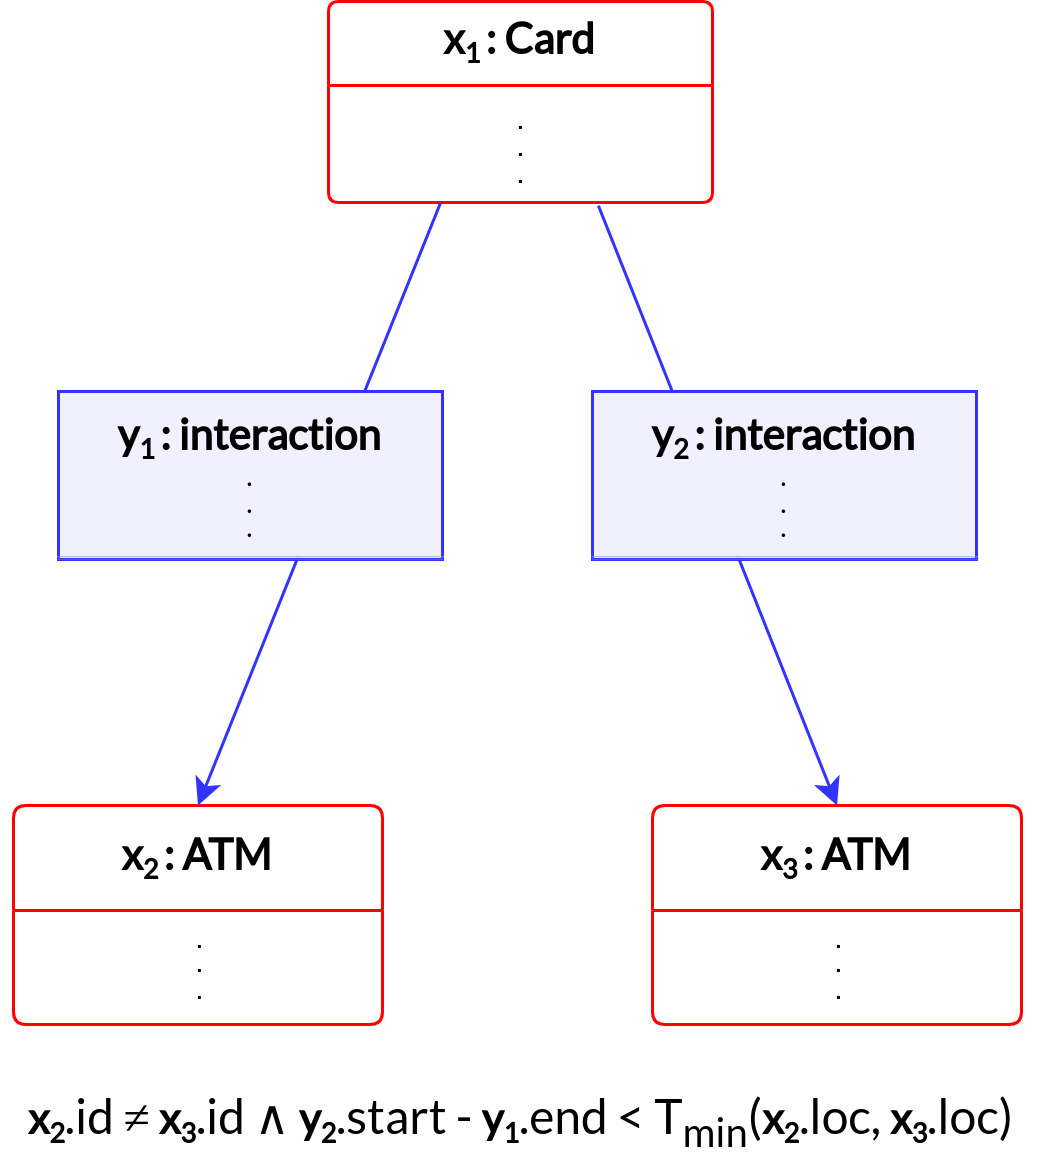
\includegraphics[scale = 0.8]{images/2-QueryModel/graphPattern-1.png}
  \caption{Property graph pattern - Card cloning characterization}
  \label{img:graphPattern-1}
\end{figure}

The pattern consists on a \texttt{Card} entity $x_1$, having two \texttt{interaction} relations $y_1$ and $y_2$ with two different \texttt{ATMs} $x_2$ and $x_3$, respectively, such that the time difference between the ending time of the first \texttt{interaction} $y_1.\textit{end}$ and the starting time of the second \texttt{interaction} $y_2.\textit{start}$, is not sufficient to cover the minimum time needed to travel from the first to the second \texttt{ATM} location $T_{min}(x_2.\textit{location}, x_3.\textit{location})$. As a whole:

$$
\small
x2.id \ne x3.id \ \land \ y_2.\textit{start} - y_1.\textit{end} < T_{min}(x_2.\textit{location}, x_3.\textit{location})
$$

where $x_2.\textit{location}$ location represents the location coordinates pair of the $x_2$ ATM: $x_2.location = (x_2.loc\_latitude, x_2.loc\_longitude)$. Same for the \texttt{ATM} $x_3$.\\

An example of this kind of anomalous card-ATM interaction, could be one as represented on Figure \ref{img:graphPattern-1-Example}, in which an ATM interaction with a certain card is finished at time 22:14 in Barcelona, and then another interaction with that same card starts at time 22:56 of that same day in Madrid. Clearly this should be reported as this kind of anomalous scenario since it is impossible, for the time being, to cover the distance between these two cities in that time difference.

\begin{figure}[H]
  \centering
  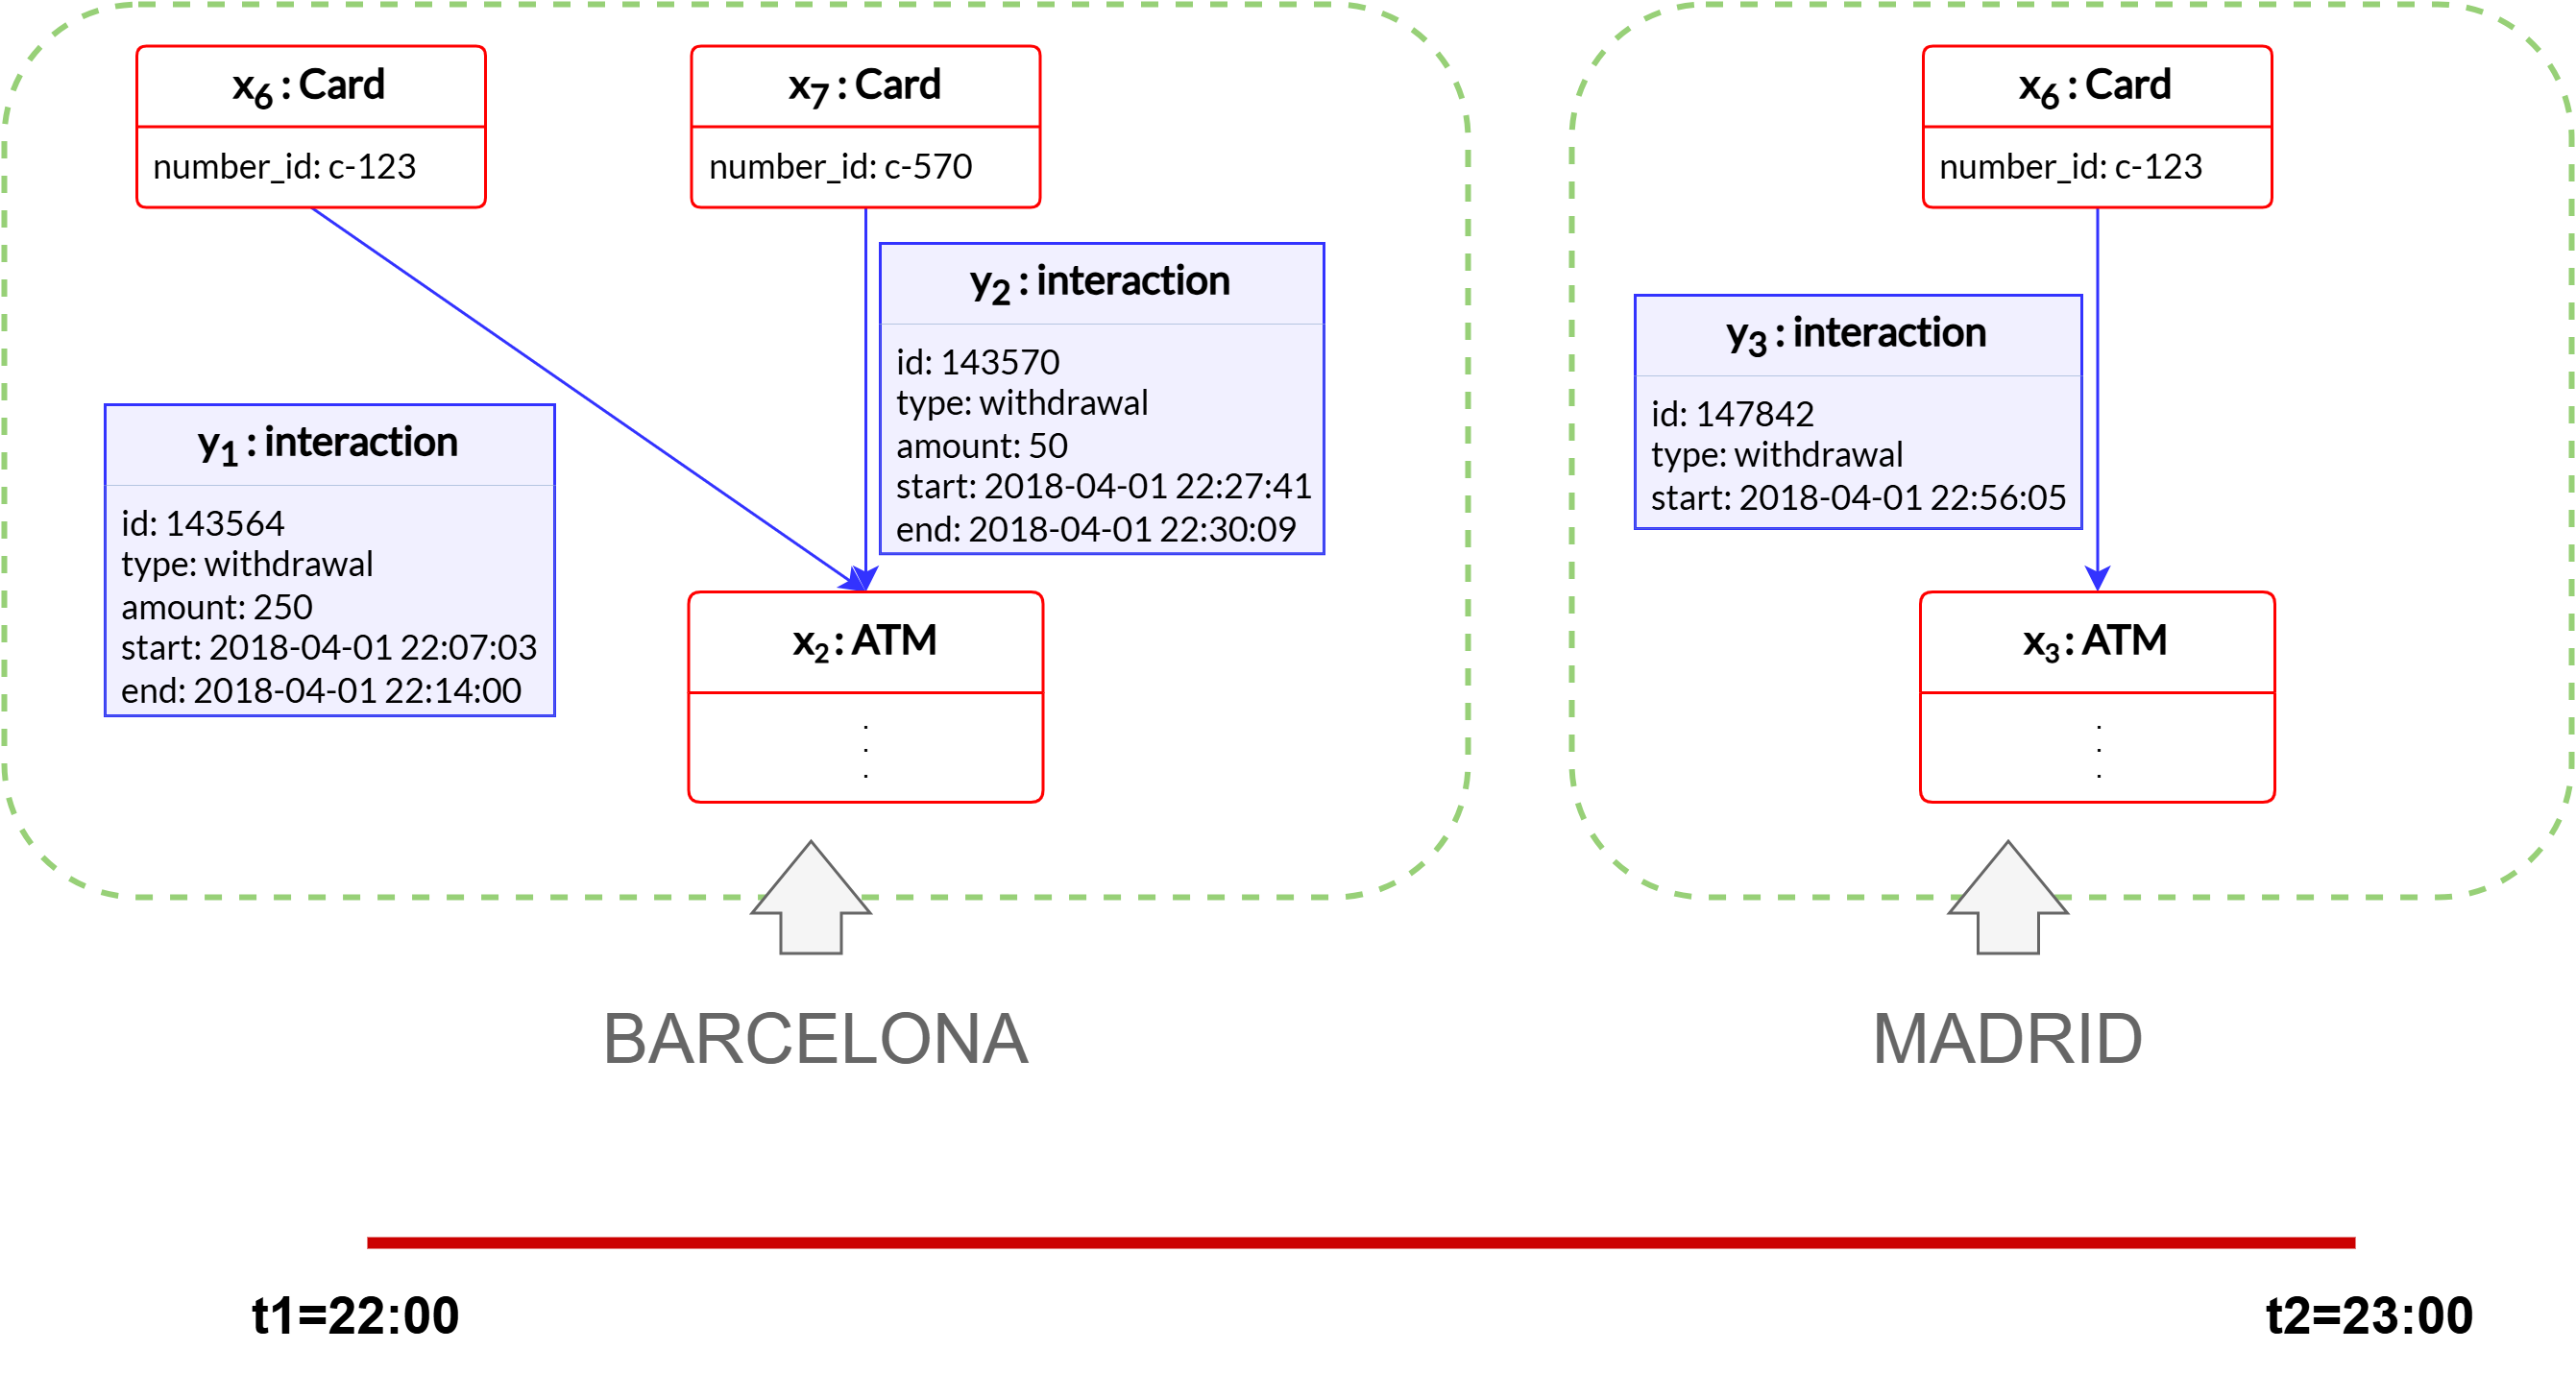
\includegraphics[scale = 0.7]{images/2-QueryModel/FP1-Example.png}
  \caption{Card cloning characterization - an example}
  \label{img:graphPattern-1-Example}
\end{figure}

\paragraph{II - Lost-and-Stolen Card Characterization\\\\}

"Lost-and-stolen card is the fraud scenario produced when a card is physically stolen or is lost, and is then used by a criminal, posing as you, to obtain goods and services" \cite{FP-lost-and-stolen-americanexpress2025}.\\

A possible way that we propose to detect this kind of fraud scenario is through the tracking of a typical behavior that it is produced when the card is used by the criminal. That is, when obtained, the fraudster tries to do as many as possible money withdrawals in different ATMs before the owner of the card realises and asks the bank to freeze the card. The detection of this kind of fraud scenario is modeled with a PG graph pattern as the one represented on Figure \ref{img:graphPattern-2}.

\begin{figure}[H]
  \centering
  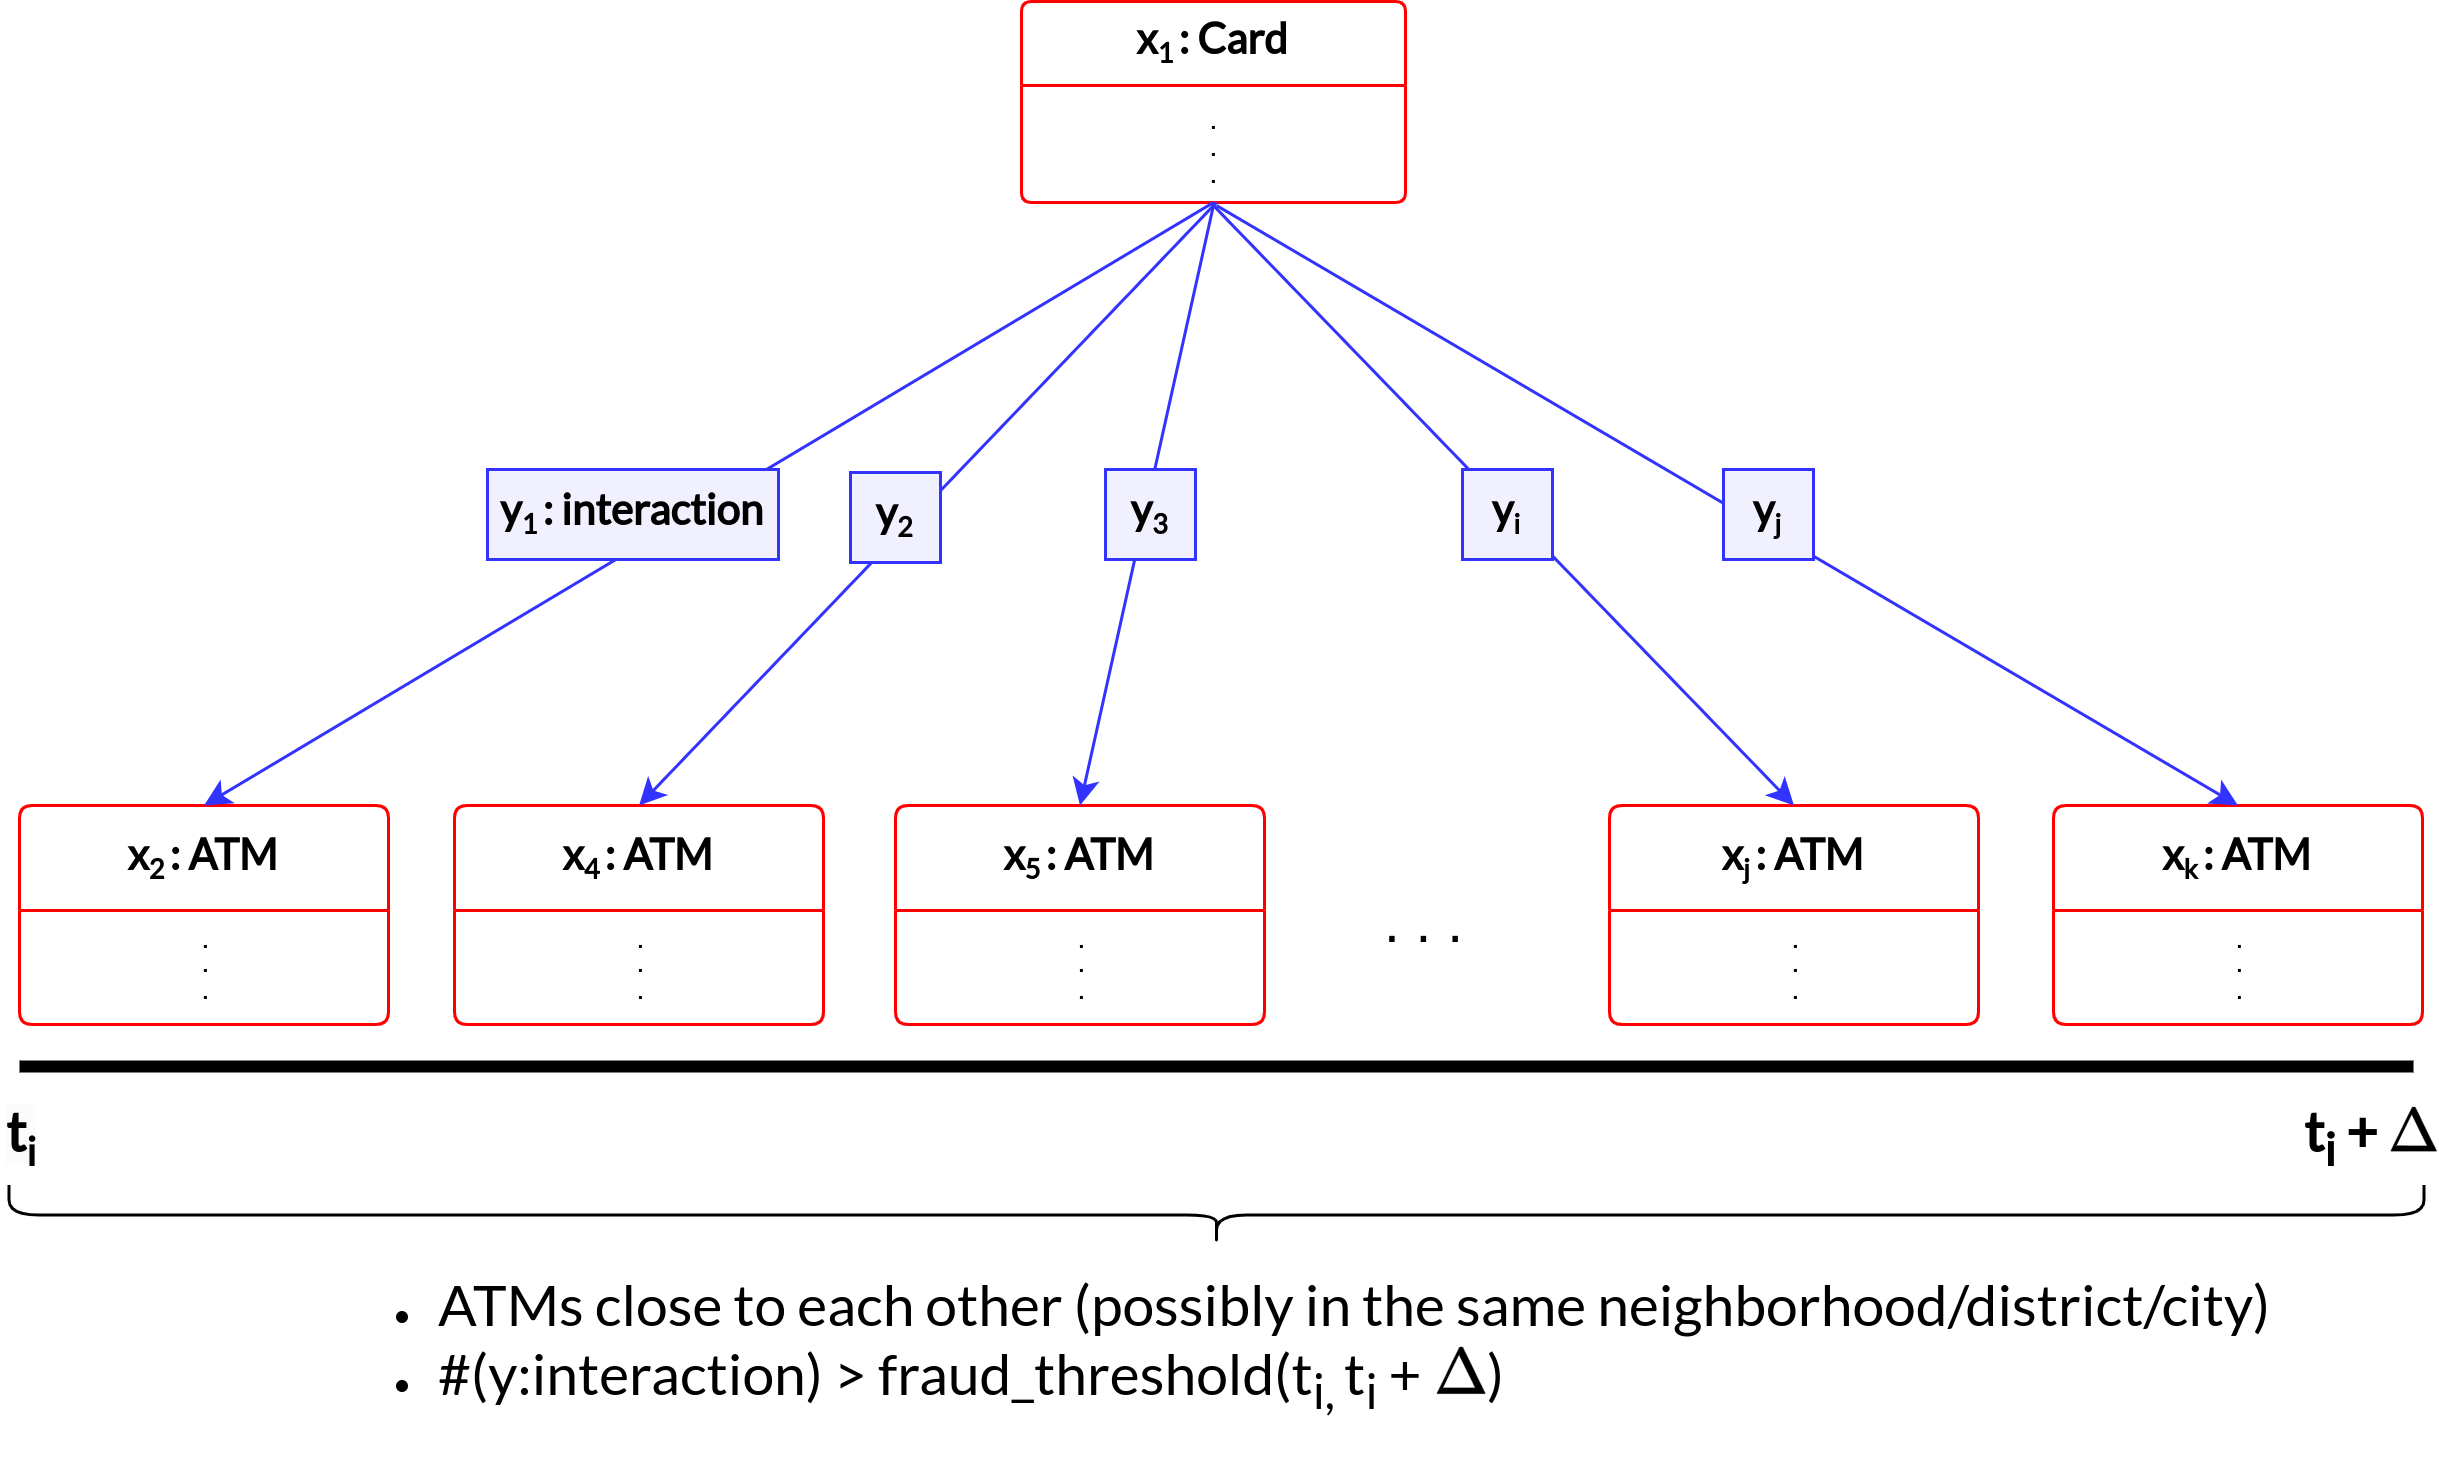
\includegraphics[scale = 0.7]{images/2-QueryModel/graphPattern-2.png}
  \caption{Property graph pattern - Lost-and-stolen card characterization. The interactions $y_1,...,y_j$ depicted are of the \emph{type} withdrawal}
  \label{img:graphPattern-2}
\end{figure}

On it we define a \texttt{Card} entity $x_1$ having a number $k$ of \texttt{interactions} $y$ at different \texttt{ATMs} $x_2 ... x_k$ within a time interval $[t_i, t_i + \Delta]$, where $t_i = y_1.\textit{start}$ and $t_i + \Delta = y_j.\textit{start}$, such that $k$ is considered to be an usual high number of withdrawals for that time interval. A reference for the usual number of withdrawals on a certain time interval for a specific cardholder can be obtained from the gathered cardholder behavior \emph{withdrawal\_day} \texttt{Card} entity property.
Another indicator of this scenario to be considered could also be the \emph{amount} value of the withdrawal operations performed, which, in these scenarios, is normally a low value to prevent that the card owner realises.

\paragraph{III - Other possible fraud scenarios\\\\}

Some other anomalous scenarios for which more graph patterns could be defined are:
\begin{itemize}
    \item \textbf{Anomalous location usage}: When a transaction is made in a location out of the threshold distance of the usual/registered address of the cardholder.
    \item \textbf{Anomalous number of operations}: Related with the II pattern characterized, we could also define a graph pattern related with a higher than average number of operations of any kind (withdrawal, inquiry, transfer or deposit) for a cardholder in a certain time interval.
    \item \textbf{Anomalous high expenses:} Similar to the II pattern, but in this case, not considering only the number of the withdrawal operations performed on a certain time interval, but the amount of the withdrawal operations on a certain time interval. This could indicate an anomalous behavior of the cardholder, withdrawing an amount of money way higher for a considered time interval.
\end{itemize}
\fi

\subsubsection*{Fraud Patterns Algorithmic Description}

So far, among all the characterized anomalous scenarios as PG graph patterns, for our proof of concept, 
we implemented the detection of the first defined fraud graph pattern, the fraud graph pattern I (defined in \ref{sub:anomalouspatterns}), 
related with the card cloning characterization.\\

A first attempt to detect fraud pattern I in our setting is to compare, for each new transaction of a given card, 
its initial time against the final time of all the previous transactions of the same card. 
This procedure is given in Algorithm \ref{alg:check-fraud-1}. 
Note that $\mathsf{S_c}$ refers to an individual node \texttt{Card} $\mathsf{c}$ subgraph of our volatile property graph. 
It stores all the card-ATM interactions $\mathsf{e_c}$ that are made with \texttt{Card} $\mathsf{c}$ for a considered time interval. 
$\mathsf{e_{new}}$ is the new incoming edge belonging to \texttt{Card} $\mathsf{c}$, such that it is an opening interaction edge. 
Note that this is this way since for the incoming closing interaction edges, we will not perform any fraud checking operation \text{CheckFraud()}.

\begin{algorithm}[H]
    \small
    \begin{algorithmic}[1]
    \REQUIRE $\mathsf{S_c}$ refers to an individual node \texttt{Card} $\mathsf{c}$ subgraph of our volatile property graph. 
    It stores all the card-ATM interactions $\mathsf{e_c}$ that are made with \texttt{Card} $\mathsf{c}$ for a considered time interval. 
    The interactions are stored sorted by time.
    \REQUIRE $\mathsf{e_{new}}$ is the new incoming edge belonging to \texttt{Card} $\mathsf{c}$
    \STATE $\texttt{fraudIndicator} \gets \texttt{False}$
    \STATE $i \gets |S_c|$
    \WHILE{$i > 0$ \AND \texttt{fraudIndicator} = \texttt{False}}
      \STATE $e_i \gets S_c[i]$
      \STATE $\texttt{t\_min} \gets \text{obtain\_t\_min}(e_i, e_{new})$
      \STATE $\texttt{t\_diff} \gets e_{new}.start - e_i.end$
      \IF{$\texttt{t\_diff} < \texttt{t\_min}$}   
        \STATE $\text{createAlert}(e_i, e_{new})$
        \STATE $\texttt{fraudIndicator} \gets \texttt{True}$
      \ENDIF
      \STATE $i \gets i - 1$
    \ENDWHILE
    \end{algorithmic}
    \caption{$\text{CheckFraud}(\mathsf{S_c}, \mathsf{e_{new}})$ -- \textbf{initial version}}
    \label{alg:check-fraud-1}
\end{algorithm}

There are some aspects and decisions of this algorithm that are worth to describe:

\begin{itemize}
    \item \textbf{Pairwise detection}. The checking of the anomalous fraud scenario is executed 
    by doing the check between the new incoming edge $\mathsf{e_{new}}$ and each of the edges $\mathsf{e_i}$ of the \texttt{Card} $\mathsf{c}$ subgraph $\mathsf{S_c}$.
    \item \textbf{Backwards order checking}. The pairs $(\mathsf{e_{new}, e_i})$ are checked in a backwards time traversal order of the edges of the $\mathsf{S_c}$ subgraph, starting with the most recent edge of the subgraph and ending with the oldest.  
    \item \textbf{Stop the checking whenever the first anomalous scenario is detected}. Whenever an anomalous scenario corresponding to a pair $(\mathsf{e_{new}, e_i})$ is detected 
    we stop the checking at this point and emit the corresponding alert. There is no need to continue the checking with previous edges of $\mathsf{S_c}$. 
    \item \textbf{Emission of the pair $(\mathsf{e_{new}, e_i})$ as the alert}. The alert is composed by the pair $(\mathsf{e_{new}, e_i})$ that is detected to cause the anomalous scenario. Both edges are emitted in the alert since we do not know which is the one that is the anomalous. On the one hand, it can be $\mathsf{e_i}$, which is previous to $\mathsf{e_{new}}$, in the case that $\mathsf{e_i}$ at the moment it arrived it did not cause any alert with the previous edges/transactions of the subgraph and it causes it now with a new incoming edge $\mathsf{e_{new}}$ which is a regular transaction of the client. On the other hand, it can be $\mathsf{e_{new}}$, which is the last edge that arrived to the system, that directly causes the alert with the last (ordinary) transaction of the card.
\end{itemize}

However, a more detailed study, lead us to observe that Algorithm \ref{alg:check-fraud-1} has two important drawbacks. 
The first one is related to the amount of memory it requires since it has to keep stored all the transactions made with every card present in the system. 
The second one is related to the execution time since every new transaction of each card has to be compared with all the previous transactions of the same card. 
To overcome the above mentioned disadvantages we propose Algorithm \ref{alg:check-fraud-def}, a simplification of the initially proposed algorithm. 
There we just perform the checking between the new incoming edge $\mathsf{e_{new}}$ and the most recent edge of the subgraph $\mathsf{S_c}$, $\mathsf{e_{last}}$.

\begin{algorithm}[H]
  \small
  \begin{algorithmic}[1]
   \REQUIRE $\mathsf{S_c}$ refers to an individual node \texttt{Card} $\mathsf{c}$ subgraph of our volatile property graph. It stores all the card-ATM interactions $\mathsf{e_c}$ that are made with \texttt{Card} $\mathsf{c}$ for a considered time interval. The interactions are stored sorted by time.
   \REQUIRE $\mathsf{e_{new}}$ is the new incoming edge belonging to \texttt{Card} $\mathsf{c}$
  \STATE $last \gets |S|$
  \STATE $e_{last} \gets S[last]$
  \STATE $\texttt{t\_min} \gets \text{obtain\_t\_min}(e_{last}, e_{new})$
  \STATE $\texttt{t\_diff} \gets e_{new}.start - e_{last}.end$
  \IF{$\texttt{t\_diff} < \texttt{t\_min}$}   
    \STATE $\text{createAlert}(e_{last}, e_{new})$
  \ENDIF
  \end{algorithmic}
  \caption{$\text{CheckFraud}(\mathsf{S_c}, \mathsf{e_{new}})$ -- \textbf{definitive version}}
  \label{alg:check-fraud-def}
\end{algorithm}


In what follows we argument the reason why it is sufficient to just check the fraud scenario among $\mathsf{e_{new}}$ and the last/most recent edge of the subgraph and not have to continue having to check with the rest of the edges.

Assume that we have a \texttt{Card} $\mathsf{c}$ subgraph $\mathsf{S_c}$ as the one depicted in Figure \ref{img:fp-I-demo}, and that we do not know if there have been anomalous scenarios produced between previous pairs of edges of the $\mathsf{S_c}$ and,
\begin{itemize}
    \item Name $\mathsf{F_I(y_i,y_j)}$ a boolean function that is able to say whether it exists an anomalous fraud scenario of this type between the pair of edges $\mathsf{(y_i,y_j)}$ or not.
    \item In addition, note that the edges of the subgraph $\mathsf{S_c}$ are ordered by time in ascending order, in such a way that $\mathsf{y_1} < \mathsf{y_2} < \mathsf{y_3}$.
    \item Finally note that $\mathsf{y_3} \equiv \mathsf{e_{new}}$ as it is the new incoming edge and $\mathsf{y_2} \equiv \mathsf{e_{last}}$, since it is the last edge / the most recent edge of $\mathsf{S_c}$.
\end{itemize} 

\begin{figure}[H]
  \centering
  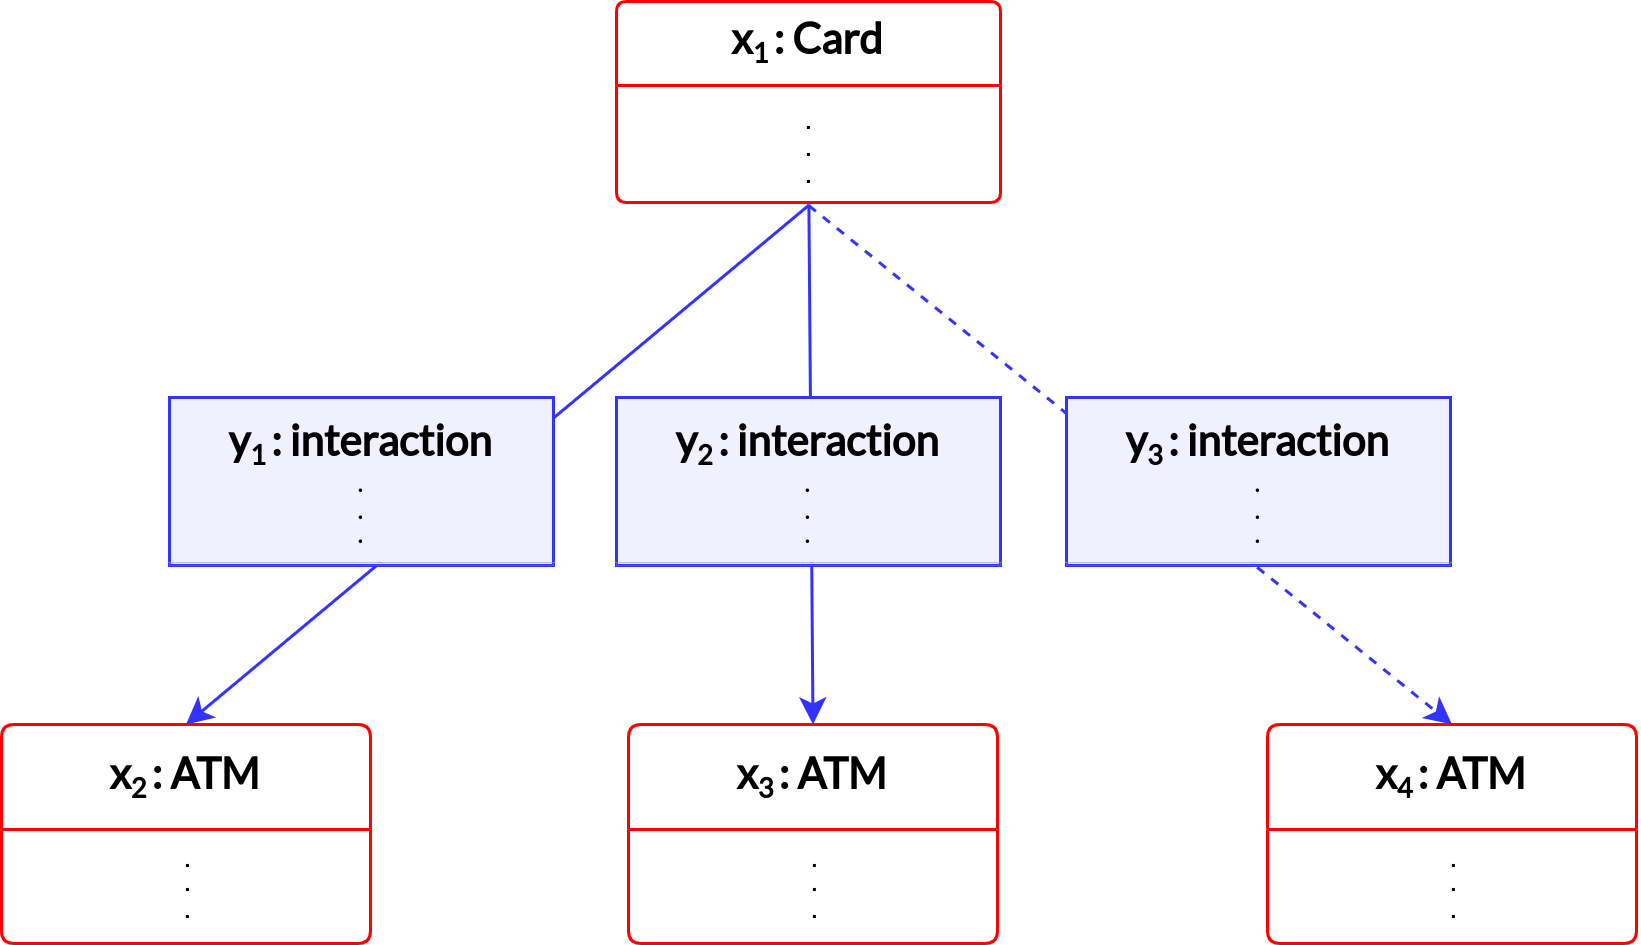
\includegraphics[scale = 0.7]{images/2-QueryModel/fp-I-demo-1.png}
  \caption{Example of a \texttt{Card} $\mathsf{c}$ subgraph $\mathsf{S_c}$ of the volatile property graph. $\mathsf{S_c}$ is an individual node \texttt{Card} $\mathsf{c}$ subgraph of our volatile property graph. It stores all the card-ATM interactions $\mathsf{e_c}$ that are made with \texttt{Card} $\mathsf{c}$ for a considered time interval. The interactions are stored sorted by time.}
  \label{img:fp-I-demo}
\end{figure}

Note that, given the above description, we can either have that:
\begin{itemize}
    \item $\mathsf{F_I(y_2,y_3)}$. Then, we emit an alert of this anomalous scenario produced between the pair $\mathsf{(y_2,y_3)}$. We could continue checking for anomalous scenarios between $\mathsf{y_3}$ and previous edges of the subgraph. However, what we consider important for the bank system is to detect the occurrence of an anomalous scenario in a certain card. Therefore, we consider that, to achieve this, it is enough to emit a single alert of anomalous scenario on this card, and not many related with the same incoming transaction of the same card.
    \item $\neg \mathsf{F_I(y_2,y_3)}$. In this case we analyze whether it would be interesting or not to continue the checking with previous edges of the subgraph, based on assumptions on the fraud checking between previous edges. In particular we can have two cases:
    \begin{itemize}
        \item $\mathsf{F_I(y_1,y_2)}$. Having this it can happen that either $\mathsf{F_I(y_1,y_3)}$ or $\neg \mathsf{F_I(y_1,y_3)}$. In the case of $\mathsf{F_I(y_1,y_3)}$, since $\neg \mathsf{F_I(y_2,y_3)}$, we can infer that the anomalous scenario detected between $\mathsf{y_1}$ and $\mathsf{y_3}$ is a continuation of the same previous anomalous scenario detected between $\mathsf{y_1}$ and $\mathsf{y_2}$. Therefore, we can conclude that this does not constitute a new anomalous scenario that would require an alert.
        \item $\neg \mathsf{F_I(y_1,y_2)}$. It can be shown that \emph{by transitivity}, having \\
        $\neg \mathsf{F_I(y_1,y_2)} \land \neg \mathsf{F_I(y_2,y_3)}
        \implies \neg \mathsf{F_I(y_1,y_3)}$. \\
    \end{itemize}
\end{itemize}

Therefore, we have seen that, it is enough to perform the checking between the pair formed by $\mathsf{e_{new}}$ and the most recent edge of the subgraph $\mathsf{e_{last}}$. $\square$\\


So, we can state that, in an implementation of the detection of the fraud pattern I, for a subgraph $\mathsf{S_c}$, it would be sufficient to only store the last incoming transaction edge $\mathsf{e_{last}}$.\\

Finally, note that due to this algorithmic method, a fraud pattern I alert could be triggered both when an anomalous interaction arrives, $\mathsf{e_{anom}}$, with respect to its previous transaction $\mathsf{e_{prev}}$, emitting the alert pair $\mathsf{(e_{prev}, e_{anom})}$; and also when the subsequent transaction $\mathsf{e_{next}}$ arrives, with respect to the anomalous, emitting the alert pair $\mathsf{(e_{anom}, e_{next})}$.

%\subsection{Architecture of the continuos query engine}


XXXXXX Gr\'afico de Javier
XXXXXx

\fmc{Explicar la idea de nuestro sistema, lo de que es un sistema para la detección de fraude a tiempo real, idea del double check para la authentication... sin entrar en mucho detalle de como lo hacemos (ya se describe en el apartado siguiente del continuous query engine). Que describa la idea / propósito / objetivo de lo que queremos hacer. Que sirva para introducir el apartado siguiente del \DPATM}

\fmc{IMPORTANTE: Buen dibujo de la arquitectura que sirva como para describir la idea del sistema que hacemos}
%
\iffalse
\begin{figure}[t!]
         \centering
         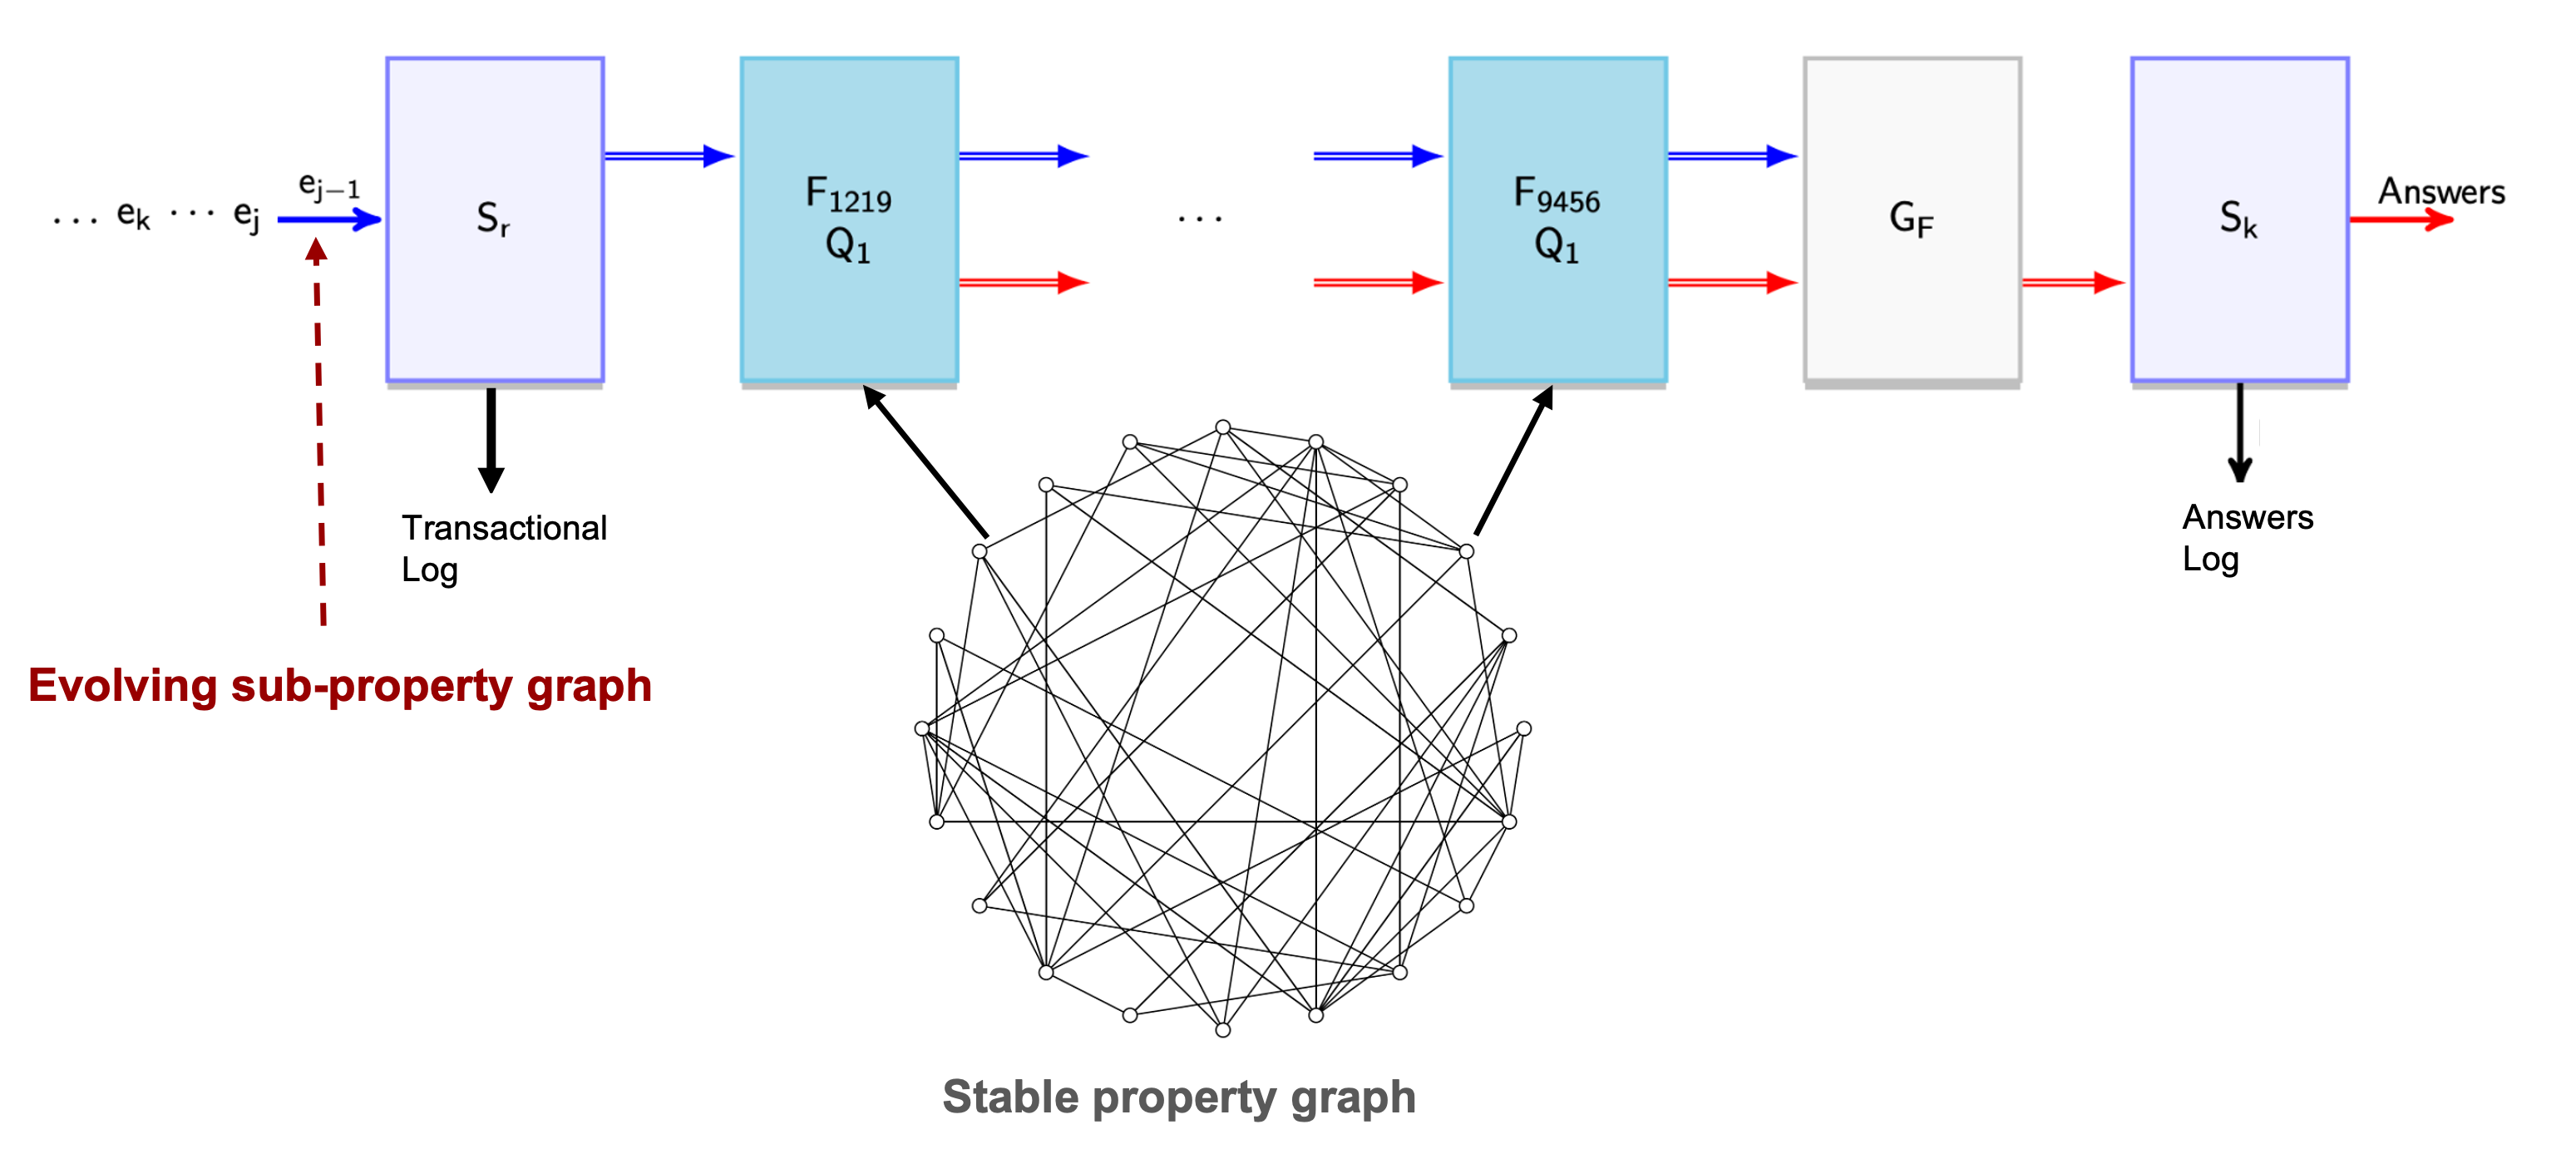
\includegraphics[width=0.7\textwidth]{images/architecture.png}
         \caption{Preliminary continuous query engine architecture for detecting anomalous ATM transactions based on the dynamic pipeline computational model. Considering the schema given in Figure \ref{fig:constinuousPGa}, in this directed (multi) graph presentation of the $\mathsf{DP_{ATM}}$, the arriving input data is a stream  $\mathsf{\langle \dots e_k\dots e_j \: e_{j-1}\rangle}$ corresponding to \textsf{interactions} (volatile relations). Boxes (vertices) represent stateful processes called \emph{stages} and internal arrows in the pipeline represent channels. Blue channels carry interaction edges and red channels carry detected anomalies (answers).  $\mathsf{S_r}$ and $\mathsf{S_k}$ correspond to the \textsf{Source} and \textsf{Sink} stages which receive input data and results, respectively. \textsf{Filter} stages, $\mathsf{F_{N}}$, are parameterized with the value of the property \textsf{number} ($\mathsf{N}$) of \textsf{Card} vertices. The \textsf{Generator} stage, $\mathsf{G_F}$, is in charge of spawning new filters, when required. The stable PG is a standard bank database (i.e. without volatile relations). Transactional log and Answers log keep input interactions and answers, respectively.
         }
         \label{fig:DP_ATM}
\end{figure}
\fi
%

%\newpage

\subsection{Dynamic Pipeline Paradigm}\label{DPP}

\textcolor{gray}{To explain:
\begin{itemize}
    \item PP (Pipeline Parallelism) computational model. The definition
    \item DP stages y un poco que hace cada stage
    \item Problemas que ya se han resuelto con este paradigma. Referenciar.
\end{itemize}
}

\fmc{Definición - Tomada de TFM Dani y J Pablo... completar mas?}

\ad{Yo creo que puedes citar ambas tesis y también el paper de Edelmira y explicar lo que es pero no hace falta que entres en demasiado detalle general, eso sí, los detalles de cómo lo usas para lo tuyo sí deben estar completos.}
In the context of Stream Processing, many data driven frameworks have emerged to address the management of continuous data streams. Dynamic data processing, characterized by the adaptive and responsive manipulation of large datasets in real time, and incremental generation of results, represent pivotal approaches.\\

One such model for Stream Processing is the Dynamic Pipeline Paradigm ($\mathsf{DPP}$) \cite{DP-pasarella2024computational}. The $\mathsf{DPP}$ is a PP (Pipeline Parallelism) data driven computational model that operates as a one-dimensional, unidirectional chain of stages connected by means of data channels. Essentially, the paradigm establishes a computational model rooted in the deployment of a linear pipeline consisting of a chain of stages structure called Dynamic Pipeline ($\mathsf{DP}$). It stretches and
shrinks depending on the spawning and the lifetime of its stages, respectively. Stages are processes that execute tasks concurrently/in-parallel.\\

\begin{figure}[H]
  \centering
  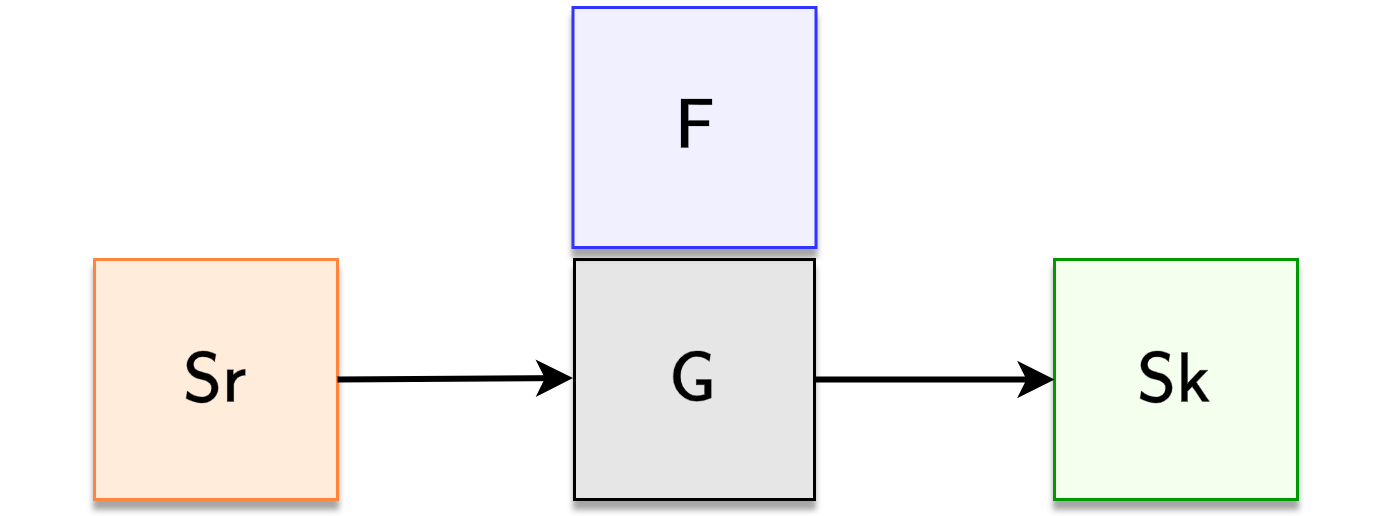
\includegraphics[scale = 0.7]{images/3-Engine/DP-Stages-1.png}
  \caption{Initial configuration of a Dynamic Pipeline. An initial $\mathsf{DP}$ consists of three stages: \emph{Source} ($\mathsf{Sr}$), \emph{Generator} ($\mathsf{G}$) and \emph{Sink} ($\mathsf{Sk}$). Above the  \emph{Generator} ($\mathsf{G}$) the \emph{Filter} ($\mathsf{F}$) parameter. The stages are connected through its channels, represented with the black right arrows.}
  \label{img:DP-Stages-1}
\end{figure}

These stages can be of four different types: \emph{Source} ($\mathsf{Sr}$), \emph{Filter} ($\mathsf{F}$), \emph{Generator} ($\mathsf{G}$) and \emph{Sink} ($\mathsf{Sk}$). \emph{Source} stage are the responsible of obtaining the input data stream and feeding it into the pipeline. \emph{Filter} stages maintain a state and process the incoming data processing it accordingly and/or passing it again to the pipeline. \emph{Generator} stage is in charge of spawning new \emph{Filter} stages when needed based on the incoming data, providing the \textit{dynamic} behavior to the model. Finally, \emph{Sink} stage receives the results, processing and acting on them as needed.
Figure \ref{img:DP-Stages-1} represents the initial configuration of a $\mathsf{DP}$ and Figure \ref{img:DP-Stages-2} depicts the stages of the $\mathsf{DP}$ after a possible evolution, where the \emph{Generator} has created two \emph{Filter} stage instances.\\

\begin{figure}[H]
  \centering
  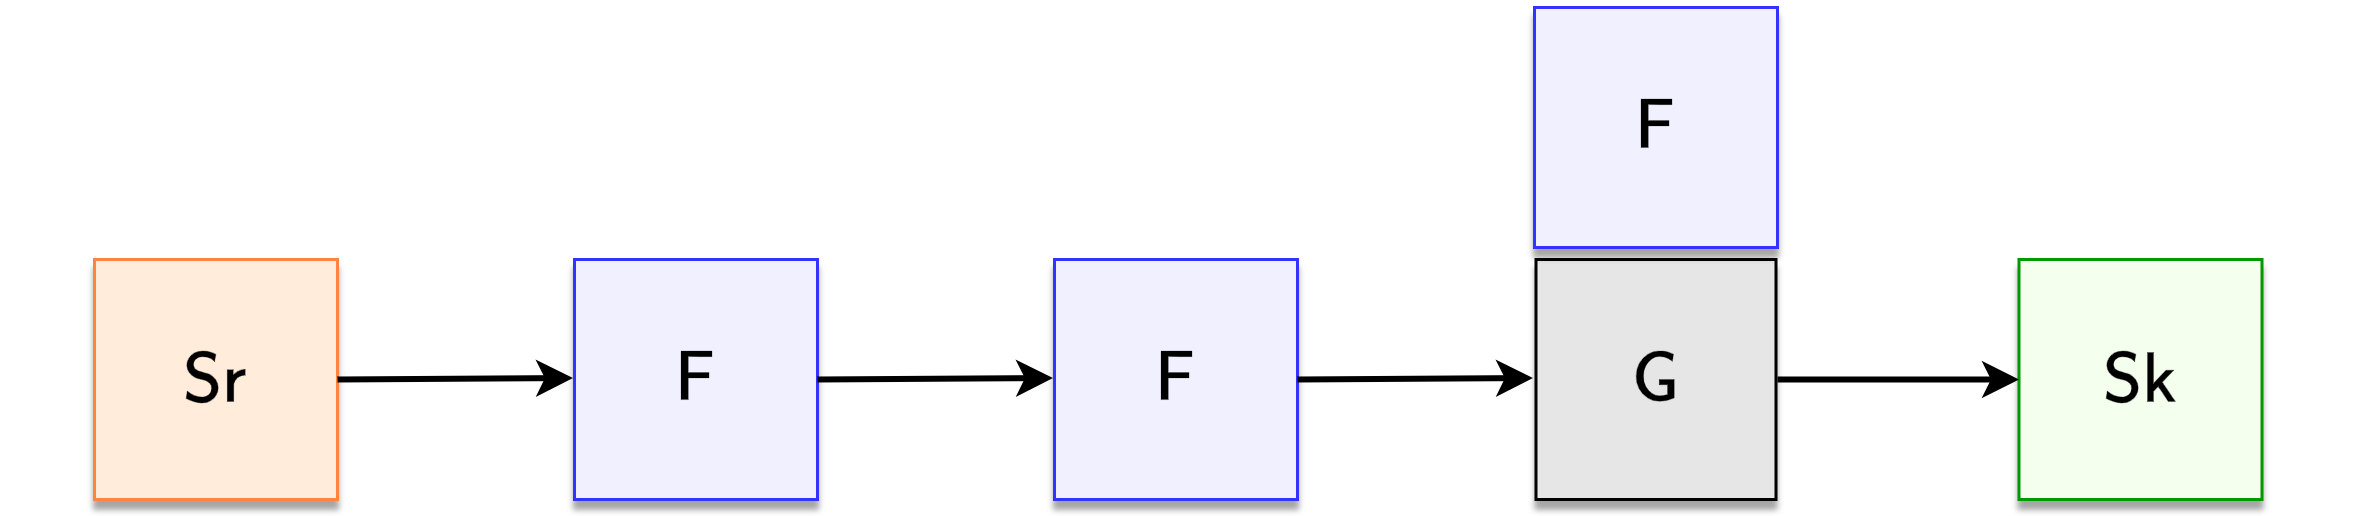
\includegraphics[scale = 0.7]{images/3-Engine/DP-Stages-2.png}
  \caption{Evolution of a $\mathsf{DP}$. After the creation of two \emph{Filter} $\mathsf{F}$ stage instances of the \emph{Filter} parameter (above the $\mathsf{G}$ stage) by the \emph{Generator} $\mathsf{G}$ stage.}
  \label{img:DP-Stages-2}
\end{figure}

The $\mathsf{DPP}$ has been used to model many different problems. In \cite{DP-bitriangles2021} they successfully solved the problem of progressively identify and enumerate bitriangles (i.e. a specific graph pattern) in bipartite evolving graphs. In \cite{DP-Lugosi_Enes_2019} $\mathsf{DPP}$ is used to model the problem of multidimensional range queries, that is, selection queries on objects in a k-dimensional space. Finally, in \cite{DP-Benedi_Garcia_2024} they solve the problem of computing and maintaining the minimum spanning tree of dynamic graphs.\\

In our case, we envision the architecture of our continuous query engine to detect anomalous ATM transactions under the $\mathsf{DPP}$, where the continuous input data stream is the stream of the bank ATM transactions, and we track the activity of a Card on a certain \emph{Filter} stage. Details on how the modeling of our problem with the $\mathsf{DPP}$ can be found in \ref{ContinuousQueryEngine}.




%\newpage

\subsection{Continuous Query Engine - $\mathsf{DP_{ATM}}$}\label{ContinuousQueryEngine}

\textcolor{gray}{To explain:
\begin{itemize}
    \item Encaje/Uso del DP para nuestro engine. Stages, qué hace cada stage (pseudocodigo/algoritmo de cada stage). Canales.
    \item Establecer algoritmos para identificar los patrones asociados a la busqueda de anomalias.
    \item Explicar la idea de que se define como para poder evaluar muchas continuous queries de forma simulatánea (pero que de momento sólo evaluamos una, para nuestro proof of concept)
    \item Detalles más técnicos - Implementación
    \begin{itemize}
        \item Descripción y evaluación del lenguage usado (golang)
        \item Graph-based query language
        \item Tools \& proper system configuration (distintas configuraciones en base al número máximo de tarjetas que contiene cada filtro...)
    \end{itemize}
    \item Windowing?
\end{itemize}
}
\ad{El windowing no lo menciones hasta las conclusiones.}

In this section we define a proper architecture of a continuous query engine for detecting anomalous ATM transactions on a continuous, unbounded, input stream of card-ATM transactions/interactions. We propose an engine that is modeled following the Dynamic Pipeline Paradigm $\mathsf{DPP}$ (see \ref{DPP}), the $\mathsf{DP_{ATM}}$, where, by definition, its architectural framework gets defined as a \DP.\\ 

\fmc{Encaje/Uso del DP para nuestro engine. Volatile subgraphs, cards, filters... Explicar la idea de que se define como para poder evaluar muchas continuous queries de forma simulatánea (pero que de momento sólo evaluamos una, para nuestro proof of concept)}

\fmc{Subgrafos}
The core idea of the \DPATM is to save and construct \emph{volatile} subgraphs of interactions for each of the cards, with the objective to keep track of the ATM transaction/interaction activity of each of the cards of the bank system. The card subgraphs are constructed with the interactions belonging to a certain card. They are defined as \emph{volatile} in the sense that the interactions that compose them are not intended to remain infinitely in the card subgraph, but only for a decided window of time. 
\fmc{Evaluación de muchos tipos de queries de forma simultanea. Un subgrafo por cada tipo de query}
These card subgraphs are the core object on which the detection queries of anomalous PG graph patterns takes place. For each card and for each continuous query pattern, a card subgraph is maintained, allowing the evaluation of many continuous different queries simultaneously. Note that, for each card, a different subgraph for each kind of continuous query is defined due to the possible many distinct time window policies for each particular kind of query.

\fmc{TODO: Poner un dibujo de un subgrafo volátil}

% Descripción general uso DP
To properly characterize the \DP architecture we need to define the configuration and behavior of each of the stages as well as the channels connecting them. The different stages are connected by two communication channels: the \eventch channel carries the interactions of the input data stream and the \alertch channel, which is a direct channel that connects each \emph{Filter} stage with the \sink stage, carries the alerts corresponding to the different possible anomalous transaction patterns detected in a \filter.

\fmc{Duda channels: sólo el de alerts o el de checks. Ahora en la impl tengo checks (incluidos los alerts). Se hizo con la idea de sacar todos los resultados de los checks para ver el continuous delivery of results en los experimentos. Ahora bien, en la impl. final yo diria que solo sacaría las alerts, para tener menos overhead y que el aviso de fraude pudiera llegar antes.}

\ad{Para explicar puedes poner el de checks y que se vea que se van haciendo muchos checks y sólo algunos provocan alerts. Luego puedes explicar que en una "working" version no se pondrías los checks para ser más eficientes y tardar menos en dar los alerts como bien dices.}

Regarding the stages, the \emph{Filter} stage is defined to be the \textit{continuous query evaluator} for a certain subset of bank cards, maintaining the subgraphs for the cards subset that are induced by the interaction edges.

% IDEA GENERAL DP-ATM flow
With this, the \DPATM algorithm overview is as follows: when an interaction $\mathsf{e}$ (with its properties' values) arrives to the \DPATM, the \source stage \Sr registers it into a standard transactional log file. Then, \Sr passes $\mathsf{e}$ to the next stage. If there exists a \filter parameterized with the value of the property \emph{number\_id} of the Card vertex $\mathsf{c}$ that is incident to $\mathsf{e}$, this \filter keeps $\mathsf{e}$ in its state, in particular adding $\mathsf{e}$ to the corresponding card subgraphs. Otherwise, the \filter passes $\mathsf{e}$ to the next stage. In the case of  $\mathsf{e}$ belonging to the \filter, this stage, as the \textit{continuous query evaluator} of the Card $\mathsf{c}$, decides if there is a match with (some of) the continuous query pattern(s) evaluated and emits an alert to the \sink \Sk reporting the finding. Hence, answers are the detected anomalies and they are emitted as they are obtained in filters. When answers/alerts arrive to \Sk, this stage post-processes and output them. In addition, \Sk maintains an answer log file. The fact that an interaction arrives to \G means that there were not previous interactions having the same value of Card property \emph{number\_id} and thus, a new filter parameterized with this new value is spawned. 

\fmc{TODO: Poner imagen de DP con filtros y cada filtro con los subgrafos}

% Descripción más concreta DP...

More detail regarding each of the stages behavior is provided next. An example of the pipeline schema of a \DPATM instance is shown in Figure \ref{img:pipeline-schema}.

\begin{itemize}
    \item \source \Sr: Receives the stream of the card-ATM interactions of the bank. Each interaction $\mathsf{e}$ is represented as an \emph{interaction} relation/edge of the volatile property graph model matching a Card and an ATM \ref{section:volatile-pg}. \Sr registers incoming interaction $\mathsf{e}$ on a transactional log file and passes $\mathsf{e}$ through the \eventch channel to the pipeline.
    \item \filter \F: \emph{Filters} are defined to be the \textit{continuous query evaluators} for a certain subset of the bank system cards. In particular each \F is defined by a subset of root parameters $V_{\mathsf{F}} = \{v_1,\ldots,v_k\}$, representing the Cards being tracked by \F. Therefore, each root represents a Card $\mathsf{c}$ where $v_i$ is the Card property \emph{number\_id} value: $v_i = \mathsf{c}$.\emph{number\_id}. Each \filter is defined to have a maximum capacity in terms of cards being tracked. This maximum capacity is defined by the parameter \emph{maxFilterSize}. This limits the maximum size of the subset $V_{\mathsf{F}}$, so that $|V_{\mathsf{F}}| \leq $ \emph{maxFilterSize}.

    With this, whenever an interaction $\mathsf{e}$ coming from the pipeline reaches \filter \F, it firsts checks whether $\mathsf{e}$ belongs to \filter \F. This is the case when $\mathsf{e}$ is incident to one of the roots of $V_{\mathsf{F}}$, $v_i$, which has the same \emph{number\_id} property value as the Card $\mathsf{c}$ of the interaction $\mathsf{e}$ ($\mathsf{e}$.\emph{number\_id}), that is when $v_i =\mathsf{e}$.\emph{number\_id}. This means that \F is currently tracking the activity of the Card $\mathsf{c}$ to which the interaction $\mathsf{e}$ belongs. 

    \fmc{Se explica cómo se tiene hasta ahora. Pero se debería de explicar una propuesta para el caso en el que se dejara de trackear la actividad de una tarjeta / cómo sería el proceso para poder destruir un filtro/reducir el pipeline.\\
    \textbf{Hasta ahora}: If the filter is not full then we add the not belonging cards to it, until it is full. This is what is done so far, since we are not considering the case to shrink the pipeline. On which some cards activity will be stopped to being tracked. \\
    TODO: Definir una posible propuesta para esto en el caso de que se hiciera... relacionado con lo de la ventana...\\
    - Spawning case is well defined.\\
    - Shrinking case idea: all the cards of the filter have to be "outdated" so that the filter can be eliminated... (not done for the moment, infinite window considered)
    }
    Another possible case on which $\mathsf{e}$ is decided to belong to \filter \F, is when, although the Card $\mathsf{c}$ of $\mathsf{e}$ is not currently being tracked by \F, it is decided to start doing it since \F still has the capacity to track more cards: $|V_{\mathsf{F}}| < $ \emph{maxFilterSize}. Therefore, card $\mathsf{c}$ is introduced as a new root parameter $v_{k+1} = \mathsf{e}$.\emph{number\_id} to $V_{\mathsf{F}}$: $V_{\mathsf{F}} = V_{\mathsf{F}} \cup v_{k+1}$. These two belonging conditions are summarized as:
    
    $$
    \mathsf{e} \in \mathsf{F} \iff 
    \left(\exists v_i \in V_{\mathsf{F}} \text{ such that } v_i = \mathsf{e}.\emph{number\_id} \right) 
    \lor \left(|V_{\mathsf{F}}| < \emph{maxFilterSize}\right).
    $$

    Otherwise ($\nexists v_i \in V_{\mathsf{F}} \text{ such that } v_i = \mathsf{e}.\emph{number\_id} \land |V_{\mathsf{F}}| = $ \emph{maxFilterSize}), \F passes $\mathsf{e}$ to the next stage.

    In the case of $\mathsf{e}$ belonging to \F, \F checks if there is a match with (some of) the continuous query pattern(s) evaluated and emits an alert(s) to the \sink \Sk. For this, $\mathsf{e}$ will be added to the corresponding card $\mathsf{c}$ subgraph(s) with root $v_i =\mathsf{e}$.\emph{number\_id}, and then perform the algorithm to test (each of) the continuous query pattern(s) with their associated card $\mathsf{c}$ subgraph(s). 

    \fmc{Esto justificarlo así?}
    For a card $\mathsf{c}$, we will store one different subgraph for each of the continuous query patterns evaluated. A different subgraph for each of the continuous query patterns is needed since the evaluation politics of each of the patterns may be different. For instance, for a specific pattern we may need to store a full list of interaction edges with some specific properties, whereas for others only the last interaction edge. Or even just some specific properties and not a subgraph of interactions. This will depend on the definition on each of the specific continuous query patterns considered.

    The test of a continuous query pattern is done by means of its associated card \emph{continuous query pattern subgraph} stored by \F and the information retrieved from the stable PG to identify patterns and solve constraints. This is, indeed, the way to evaluate continuous queries.
    
    \item \generator \G: Is the stage in charge of stretching the pipeline by spawning new \filter \F stages when needed. In particular this is the case whenever an interaction $\mathsf{e}$ arrives to \G. At this point this means that there was no \F in the pipeline to which this interaction belonged. That is, whenever no \F was tracking the activity of the Card $\mathsf{c}$ with property value \emph{number\_id} to which this interaction corresponds and all the running \F were full of capacity in terms of the number of maximum cards \emph{maxFilterSize} that they can track. In this case a new \F is spawned, initially tracking the activity of this Card $\mathsf{c}$ with property value \emph{number\_id} and creating new card subgraphs with the interaction $\mathsf{e}$. 
    \item \sink \Sk: It is in charge of receiving all the alerts coming from the \filter stages and to correspondingly act on them as the bank requires. This could be done in terms of communicating the alert to the corresponding cardholders, emitting a message for validating that the operation was done by the owner, freezing the corresponding cards, and so on. This will have to be defined by the corresponding bank as desired. In any case, \Sk maintains an answer log file where all the emitted alerts are registered. Additionally, an event log file is maintained, to register other internal system events.
\end{itemize}


\begin{figure}[H]
    \centering
    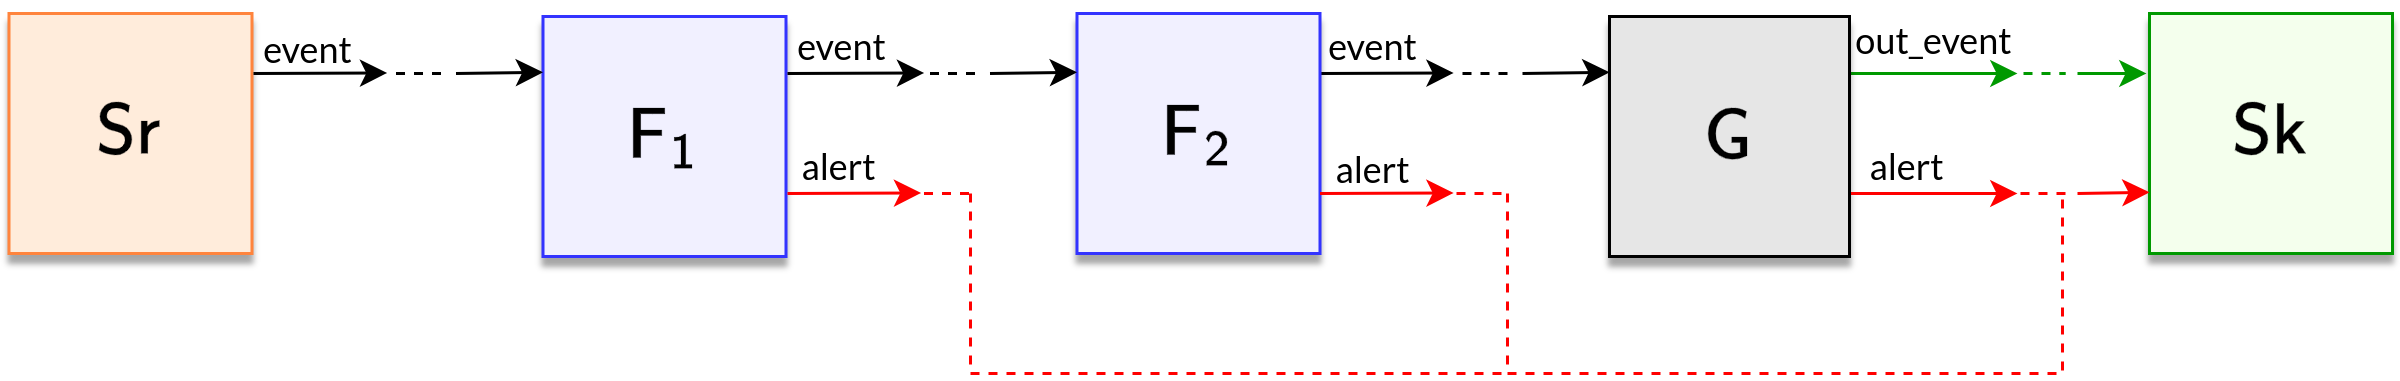
\includegraphics[scale = 0.8]{images/3-Engine/DP-2f.png}
    \caption{Example of the Pipeline Schema of a \DPATM Instance}
    \label{img:pipeline-schema}
\end{figure}


\fmc{Windowing?}
When the time interval window is over, the $\mathsf{DP_{ATM}}$ is, in some sense, reset according to the given window policy. Note that the window policy must take into account stored data that might be valid in between two windows and handle the transition properly.

\fmc{Detalles técnicos - Implementación}
\subsection*{$\mathsf{DP_{ATM}}$ - Implementation}\label{ContinuousQueryEngine-Implementation}

% Lenguaje de programación. Base de datos. Conexión a base de datos.
% - Go: Detalles versión. Por qué lo usamos
% - Neo4j: Detalles versión. Por qué lo usamos
The implementation of the proof of concept can be found in Github\footnote{\url{https://github.com/FCanfran/ATM-DP}}. It was developed using the version \texttt{1.20} of the \texttt{Golang} language. 
% Ventajas: hilos verdes - concurrencia, comunicación entre stages con canales de fácil manejo, fácil conexión con Neo4j mediante el driver
One of the main reasons why we decided to use this language is its inherent capacity to support concurrent programming \cite{Go-cbtnuggets_concurrency, Go-medium_concurrency, Go-reliasoftware_concurrency}, which is the computing technique that we need to implement the \DP schema for our \DPATM engine. In \texttt{Go}, concurrency is achieved primarly through \texttt{goroutines} and \texttt{channels}. \texttt{Goroutines} are lightweight, independent concurrent green threads, which are managed by the \texttt{Go} runtime scheduler, and enable concurrent execution of functions, in our case stages. The communication between \texttt{goroutines} is accomplished via different channels. This provides a safe and efficient method to pass complex data between the different \texttt{goroutines}. 
Unlike traditional threads, \texttt{goroutines} have a small memory footprint and can be created in large numbers with minimal overhead. The \texttt{Go} runtime includes an efficient scheduler that multiplexes \texttt{goroutines} onto CPU cores, reducing context switching overhead and optimizing resource use. However note that, \texttt{goroutines} are not inherently parallel. By default, \texttt{Go} uses only one operating system thread, regardless of the number of \texttt{goroutines}. We need to set up the \texttt{GOMAXPROCS} \footnote{\url{https://pkg.go.dev/runtime\#GOMAXPROCS}} environment variable to the number of logical processors, to achieve that the \texttt{Go} runtime scheduler multiplexes the \texttt{goroutines} onto all the possible logical processors specified.\\

Another advantage that made the election of \texttt{Go} quite suitable was its easy form to interact with \texttt{Neo4j}. \texttt{Go} provides the \texttt{Neo4j Go driver}\footnote{\url{https://neo4j.com/docs/go-manual/current/}} to easily interact with a Neo4j instance through a \texttt{Go} application. More details regarding the connection are later explained. 

\subsubsection*{Neo4j Connection}\label{Neo4j-connection}
% Detalle de la conexión con Neo4j
Our \DPATM system needs a way to interact with the stable bank database PG instance in order to retrieve additional information related with the cardholders or ATMs for the evaluation of the continuous queries. The connection to the Neo4j graph database instance that represents the stable bank PG database is implemented using the version \texttt{v5.24.0} of the \texttt{Neo4j Go driver}\footnote{\url{https://pkg.go.dev/github.com/neo4j/neo4j-go-driver/v5@v5.24.0/neo4j}}. Next we give an overview of some important details on the usage of this driver in order to connect and query the Neo4j instance. More detail on the methods we used can be found in the official driver module websites \cite{neo4j-go-neo4j_go_driver, neo4j-go-neo4j_go_manual}.\\


In our implementation of the \DPATM system in \texttt{Go} we developed the \texttt{Go} module \texttt{internal/connection} to deal with the connection management with the Neo4j stable bank graph database instance.
On it we provide all the needed functions to connect to the database, create connection sessions, and to query it. 

% Initial connection method - .env... driverwithcontext
% Sessions for each of the filters
% Query method to run cypher queries...

\begin{itemize}
    \item \textbf{Initial connection setup}: The \DPATM system initially sets up the connection through the creation of a \texttt{DriverWithContext} object.\\
    In the \texttt{internal/connection} module \texttt{SafeConnect()} is the function that we implement to construct the \texttt{DriverWithContext} object and verifies that a working connection can be established through the \texttt{.VerifyConnectivity()} method.
    The \texttt{DriverWithContext} object holds the details required to establish connections with a Neo4j database, allowing connections and creation of sessions. It is a sharable object among threads. To provide the required details we used the module package \texttt{godotenv}\footnote{\url{https://pkg.go.dev/github.com/joho/godotenv}} to obtain the \textit{URI} and the credentials from a \texttt{.env} file, where the related environment variables are specified. For the connection with our Neo4j instance we use the \texttt{Bolt}\footnote{\url{https://neo4j.com/docs/bolt/current/bolt/}} application protocol, which is the protocol used for interaction between Neo4j instances and drivers. It listens on port 7687 by default. 
    To illustrate, we show an example of a \texttt{.env} file, from which the connection credentials will be gathered by our application. On it the connection details of a toy local Neo4j instance are shared:

    \begin{center}
    \lstset{style=cypherStyle}
    \begin{lstlisting}[caption={Example of a \texttt{.env} file, from which from which the connection credentials will be gathered by our \DPATM application.}]
        NEO4J_URI="bolt://localhost:7687"
        NEO4J_USERNAME="neo4j"
        NEO4J_PASSWORD="xxxxx"
    \end{lstlisting}
    \end{center}

    \item \textbf{Connection sessions}: \texttt{Sessions} act as concrete query channels between the driver(\texttt{DriverWithContext} object) and the server. We need them in order to be able to run \texttt{Cypher} queries from each of the working \filter stages. Each \filter stage creates a different \texttt{session} to interact with the Neo4j database.
    
    In the \texttt{internal/connection} module, the functions \texttt{CreateSession(...)} and \texttt{CloseSession(...)} are the functions for the creation and closing of a \texttt{session}.
    They are created from the \texttt{DriverWithContext} object. 

    \item \textbf{Running queries}: We provide the methods \texttt{ReadQuery(...)} and \texttt{WriteQuery(...)}, which create a \textit{managed transaction} to retrieve data from the database or alter it, respectively, through a \texttt{Cypher} statement. 
    Internally they call the \texttt{ExecuteRead(...)} and the \texttt{ExecuteWrite(...)} functions of the \texttt{Neo4j Go Driver}, which execute the given unit of work in a read/write transaction, via the provided session.

    In the \DPATM we make use of the \texttt{ReadQuery(...)} function from each of the \filter stages, using its own \texttt{session}, to query the database using \texttt{Cypher} statements.
\end{itemize}

\fmc{DUDA: Pongo una referencia a esto?}
\textcolor{gray}{Neo4j limits the number of parallel transactions to 1000 by default. However, so far no reference regarding the limit on the number of parallel sessions has been found. In any case, it is important to remark that many multiple parallel sessions may cause overhead to the database. This can be the case for the architectural design we are proposing, where we have a session per each \filter stage.}

% Comunicación. Canales, tipos más concretos. Eventos, tipos de eventos concretos. Start and End Edges.
\subsubsection*{Communication}

The communication of the different stages is carried via different \texttt{Go} channels. In general, although otherwise specified all the channels that we use are buffered channels of size 5000. All the channels are described next:

\begin{itemize}
    \item \eventch: \texttt{event} channel. Its main purpose is to carry the interaction edges across the \DP stages, from \Sr to \G, passing by all the \F's. The \texttt{event} data type consists on a \texttt{EventType} label and in a \texttt{Edge} object. The \texttt{EventType} label indicates the type of event that can be either: \texttt{EdgeStart} representing an opening of an interaction, \texttt{EdgeEnd} representing an interaction closing, \texttt{EOF}, representing the \textit{End Of File} event so that the \DP can become to an end, finalizing all the stages, and the \texttt{LOG} event for internal log messages of the system.
    \begin{center}
    \lstset{style=golangStyle}
    \begin{lstlisting}[caption={\texttt{Event} Data Type}]
                type Event struct {
            	   Type      EventType
            	   E         Edge
                }
    \end{lstlisting}
    \end{center}

    \texttt{Edge} is the data type that we defined for the interaction edges. This object will be relevant in the case of the \texttt{EdgeStart} and \texttt{EdgeEnd} events, since in this case the \texttt{Edge} object will be containing the information of the opening and closing interaction, respectively, as defined in the volatile property graph data model definition (see \ref{section:volatile-pg}).
    
    % Tipo de dato interaction edge Edge
    \begin{center}
    \lstset{style=golangStyle}
    \begin{lstlisting}[caption={Data Type for the interaction edges in Go}]
    type Edge struct {
    Number_id string   // Card id
    ATM_id   string    // ATM id
    Tx_id    int32     // id
    Tx_type  TxType    // type (withdrawal/deposit/inquiry/transfer)
    Tx_start time.Time // start datetime(DD/MM/YYYY HH:MM:SS)
    Tx_end   time.Time // end datetime(DD/MM/YYYY HH:MM:SS)
    Tx_amount float32  // amount
    }
    \end{lstlisting}
    \end{center}

    where \texttt{TxType} is a custom type made for the different interaction types: 
    \texttt{withdrawal}, \texttt{withdrawal}, \texttt{withdrawal} and  \texttt{withdrawal}. 

    \begin{center}
    \lstset{style=golangStyle}
    \begin{lstlisting}[caption={\texttt{TxType} Data Type, for the different interaction types}]
            type TxType uint8
            const (
            	Withdrawal TxType = 0
            	Deposit           = 1
            	Inquiry           = 2
            	Transfer          = 3
            	Other             = 4
            )
    \end{lstlisting}
    \end{center}
    
    \item \alertch: \texttt{alert} channel. It carries the alerts corresponding to the different possible anomalous transaction patterns detected in a \filter. It is a channel directly connecting each of the \emph{Filters} with the Sink stage. This means that when an alert is emitted it does not have to travel through all the remaining \F stages of the \DP nor the \G stage, allowing a faster communication of the alert to the \Sk stage, in charge of processing the alerts. The \texttt{alert} data type consists on a \texttt{Label} to indicate the type of fraud pattern to which it corresponds, an \texttt{Info} string to indicate additional information related with the alert, and finally \texttt{Subgraph}, the subgraph data structure that triggered the alert. Note that this subgraph does not need to be the full subgraph of the card that triggered the alert, it can be just the part of it involved in the alert. For instance, in the case of the fraud pattern I, these subgraph is composed of the two interaction edges that caused the trigger of this kind of fraud pattern alert.
    \begin{center}
    \lstset{style=golangStyle}
    \begin{lstlisting}[caption={\texttt{Alert} Data Type}]
    type Alert struct {
    	Label    string        
    	Info     string        
    	Subgraph Graph         
    }
    \end{lstlisting}
    \end{center}
    \item $\mathsf{out\_event}$: direct dedicated \texttt{event} channel between the \G and \Sk. 
    \item $\mathsf{internal\_edge}$: Internal \texttt{event} channel between a \F stage and its related \FW substage. It only pass interaction \texttt{Edge} events (\texttt{EdgeStart} and \texttt{EdgeEnd}), that have been determined to belong to the \filter, so that the related \FW of \F can do the corresponding processing with it.
  \end{itemize}

% Detalle de las estructuras y los métodos usados en cada una de las stages.
\subsubsection*{Stages}
In what follows we give specific implementation details of each of the stages of the \DP paradigm used for the \DPATM. Each stage takes the form of a \texttt{goroutine} of the \texttt{Go} language.

% - Source: como se hace la lectura. Como se empezó haciendo inicialmente y cómo se decidió hacer finalmente (lectura por chunks) - hacer referencia a apartado de experimentos donde mostrar el experimento hecho para enseñar que era mejor.
\paragraph*{Source\\ }

% Explicar función

\source stage is designed to be the connection point of the \DPATM with the bank ATM network to receive the interactions produced on these ATMs, which compose the input interaction stream.\\

\fmc{DUDA: Aqui esto no se como ponerlo...
- Decir algo de kafka message queue (como en seraph)?
}
% Forma real de cómo sería el source: recibiendo flujo de transacciones en real time
% Cómo lo hacemos nosotros - lectura de fichero - y variantes dependiendo del tipo de experimento que realizamos
In a real-case scenario, these interaction events could be sent by the ATMs of the bank network and be received by a message queue on our \DPATM system. For our proof of concept, where we generated our own synthetic stream of transactions in a \texttt{csv} file,
the interactions are read from these files, parsed into \texttt{Edge} data types and provided to the pipeline in different ways depending on the kind of simulation we perform. As it will be shown in the Experiments section, we implemented two different cases of simulations. The real-case scenario and the high loaded test scenario. In the first case, the interactions, although read by a file of artificial simulated interactions, are provided to the pipeline data stream in such a way that they simulate their actual arrival time to the system, with the corresponding time separation between them. In the second case, the interactions are provided just one after the other as fast as possible as they are read.\\

% Cómo se leen, parsing al tipo de dato Edge...
In any case, we want the reading of the input file to be the fastest possible, so to minimize the potential bottleneck derived from the operation of reading a file, we utilized a buffered reader of the \texttt{bufio} package, which reads chunks of data into memory, providing buffered access to the file. This buffered reader was provided to a \texttt{csv} reader of the \texttt{encoding/csv} package to read the buffered stream as \texttt{csv} records.

    \begin{center}
    \lstset{style=golangStyle}
    \begin{lstlisting}[caption={\texttt{csv-bufio} reader}]
        reader := csv.NewReader(bufio.NewReader(file))
    \end{lstlisting}
    \end{center}
    
% Lectura por chunks
% chunk size = 100
% read with the help of a worker to keep reading in the background, to accelerate the reading -> explain the reason of why this
Another optimization that was done in order to be able to minimize this bottleneck on the reading of the interactions from the \texttt{csv} file, was reading by chunks the \texttt{csv} records/rows. In particular, this was done by having a \textit{worker} subprocess, implemented as an anonymous \texttt{goroutine} inside \Sr, whose task was to continuously read records from the file using the \texttt{csv-bufio} reader accumulating them in a chunk of rows that were provided through a channel to \Sr whenever they reached the defined \emph{chunkSize}. These records were read directly as \texttt{string} data types. On its side, whenever \Sr receives a chunk of rows, it takes each of the rows on it, parses it to the \texttt{Edge} data type and sends it through the pipeline to the next stage.\\

The \emph{chunkSize} was selected to be of $10^2$ rows. In \ref{input-reading} we provide an experimental analysis that proves and justifies the benefits of this buffered and chunked file reading. On it the \texttt{encoding/csv} package performance is compared to other variants using the \texttt{apache/arrow} package with different combinations of \emph{chunkSize}. We also analyze the benefits of introducing the \textit{worker} subprocess to perform the chunked reading.

\fmc{Explicar más en detalle como va lo de la lectura por chunks con el worker?}







% - Filter: forma inicial - sin filter worker y 1 card per filter - y mejoras posteriores con filter-worker y varias cards por filtro con un hash map para indexar... Poner esquema/algoritmo final del filtro (con referencia al algoritmo de FP definido en el query model).
\paragraph*{Filter\\}

Regarding the \filter stage, there are four main aspects worthy to describe on its implementation: the card subgraph data structure implementation, the \emph{decoupled event handling} implementation, the \filter multiple cards support and the continuous query evaluation.
\begin{itemize}
    \item \textbf{Card Subgraph Data Structure}\\
    It contains the interaction edges related with the continuous query fraud pattern evaluation of a specific card.
    The card subgraph data structure is selected based on the fraud patterns considered so far. Although for the implementation of the detection of the fraud pattern I (see \ref{section:queryModel}) we only need to store the last/most recent interaction for each card, we propose a \texttt{Go} \texttt{list} of \texttt{Edge} (interaction edges) objects as a more general data structure to store incoming interactions ordered by timestamp. This decision responds to what we see it is a more general data structure ready for its usage when implementing the detection of other kinds of fraud patterns.\\ 

    \begin{center}
    \lstset{style=golangStyle}
    \begin{lstlisting}[caption={Card Subgraph Data Structure in Go}]
    type Graph struct {
    	edges *list.List 
    }
    \end{lstlisting}
    \end{center}

    A card subgraph is constructed based on the belonging interaction edges that arrive in the form of incoming \texttt{EdgeStart} and \texttt{EdgeEnd} events. \texttt{EdgeStart} event  produces the creation of a new \texttt{Edge} on the data structure, whereas a \texttt{EdgeEnd} event completeS the values of the properties of the corresponding \texttt{Edge} on the data structure, that was previously created by the \texttt{EdgeStart} event corresponding to that same ATM-Card interaction.

    \fmc{TODO: Poner dibujito de subgrafos dentro del filtro?}

    \item \textbf{Decoupled Event Handling}\\
    % Filter worker
    We implement a \emph{Decoupled Event Handling}, as in the \DP implemented on \cite{DP-Benedi_Garcia_2024}. As the authors mention in this work, there exists a potential inefficiency in the way that the \filter \F stage is defined to work: if an event belongs to the filter then it does the processing related to it. Until \F does not complete this processing the events that arrive to it are not being able to be handled, even if the event does not belong to \F. We have the same scenario for the \DP of the \DPATM, where the events that can belong to \F are the interaction edge $\mathsf{e}$ events.

    To avoid this bottleneck on the flow of interaction edge $\mathsf{e}$ events, the \filterworker \FW is introduced as a substage of the \filter \F stage. \F and its associated \FW will be running in different \texttt{goroutines}. The idea is that \F acts as a dedicated \textit{mailbox}, reading the events coming from the \texttt{event} channel and \emph{filtering} them, that is, deciding whether an incoming interaction edge $\mathsf{e}$ belongs to \F or not. In the case $\mathsf{e}$ belongs to \F, \F forwards $\mathsf{e}$ to the \FW, otherwise it continues passing $\mathsf{e}$ through the pipeline. \FW is dedicated to do the corresponding processing with the interaction edges belonging to the stage that are forwarded by \F.\\

    This decoupling allows to do the processing of belonging interaction edges while not blocking the pipeline event flow, since at the same time it does the \emph{filtering} of events.\\

    In our \texttt{Go} implementation, we decided to implement \FW as an internal anonymous \texttt{goroutine} of the \F \texttt{goroutine}, instead of an external (named) \texttt{goroutine}. 

    To communicate the interaction edges between \F and \FW we use an internal channel \internaledgech. Another possible option considered was a shared buffer of interaction edges. In this last case a mutex would have been needed, since \F and \FW can possible write and read, respectively, into this buffer at the same time. The \textit{mutex} is needed to avoid race conditions in the sharing of the buffer. 
    However, channels are a much more simple alternative to lead with this communication, as they are specifically designed for synchronization and passing the ownership of data, which is the case we are dealing with. Some references on the preference usage of channels over mutex \cite{Go-channels-mutex-gowiki_mutex_channel, Go-channels-mutex-stackoverflow_mutex_channel}.

    The decision to implement \FW as an internal anonymous \texttt{goroutine} also provided a way to simplify the code, since \FW can access the variables of the scope of \F (no need to pass them as parameters). This is particularly useful in the case of the \alertch channel, to which \FW is able to write directly. Same in the case of the \internaledgech channel.

    \begin{figure}[H]
      \centering
      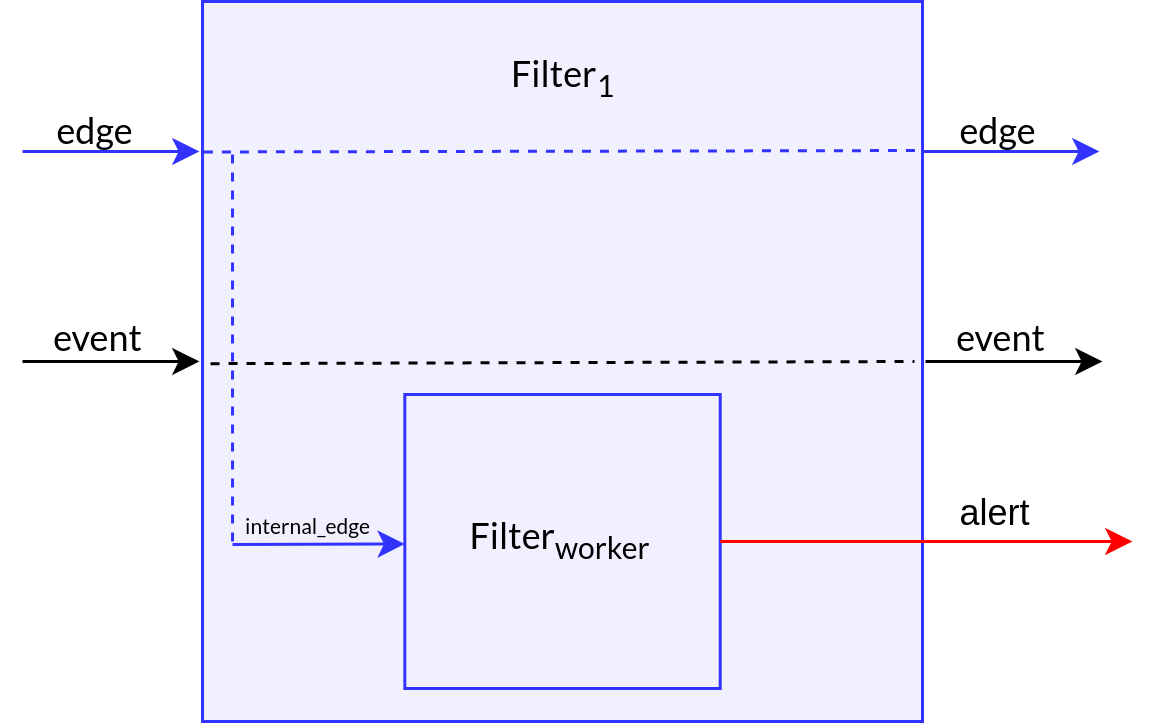
\includegraphics[scale = 1.2]{images/3-Engine/filter-worker.png}
      \caption{Filter Worker detail}
      \label{img:pipeline-schema}
    \end{figure}

    \item \textbf{Multiple Cards Support}\\
    In an initial first toy implementation, we were tracking the activity of only one card per \filter, meaning that for each bank card we were dedicating a \texttt{goroutine} on the form of a \filter stage. This was done as a way to get started, it fast became obvious that this is was an unnecessary waste of computational resources. On a real case scenario, where the number of ATM-card interactions a bank card in a day is not expected to be higher than one on average \fmc{TODO: Poner una referencia formal}, it became clear the need of allowing to share each \filter stage for multiple bank cards.\\

    Formally, as described on \ref{ContinuousQueryEngine}, each \filter \F was implemented to be able to hold a certain subset of root parameters $V_{\mathsf{F}} = \{v_1,\ldots,v_k\}$, representing the Cards being tracked by \F.\\

    In \texttt{Go} to achieve the support of multiple cards per \filter we decided to use hash tables. Go provides a built-in \texttt{map} type that implements a hash table\footnote{\url{https://go.dev/blog/maps}}. We used two different maps, using the card id of the interaction edge $\mathsf{e}$.\emph{number\_id} as the key of both maps.

    \begin{itemize}
        \item \texttt{cardList} \texttt{map}: It is used by \F to determine whether an interaction edge $\mathsf{e}$ belongs to \F, $\mathsf{e} \in$ \F. Only accessed by \F.
        \item \texttt{cardSubgraph} \texttt{map}: To index the interaction edge $\mathsf{e}$ to the corresponding card subgraph.
        Only accessed by \FW. Note that, for our proof of concept, as we are considering only one fraud pattern, we only need one \texttt{cardSubgraph} \texttt{map} data structure. However, note that more will be needed if we consider more fraud patterns with different card subgraphs.
    \end{itemize}

    \begin{center}
    \lstset{style=golangStyle}
    \begin{lstlisting}[caption={Hash Tables \texttt{map} Data Structures on a \emph{Filter} \F stage}]
    var cardList map[string]bool = make(map[string]bool)
    var cardSubgraph map[string]*cmn.Graph = make(map[string]*cmn.Graph)
    \end{lstlisting}
    \end{center}

    % Reason why two maps and not only one
    One could think of using one single \texttt{map} data structure to do the check $\mathsf{e} \in$ \F and at the same time index $\mathsf{e}$ to the corresponding card subgraph, if it is the case. However, the reason why we need two \texttt{maps} and not only one is to respect the architecture of the decoupled event handling. On it, we have two \texttt{goroutines} \F and \FW (as an anonymous internal \texttt{goroutine} of \F) dedicated to check $\mathsf{e} \in$ \F and to do the processing of $\mathsf{e}$, respectively. Having only one \texttt{map} data structure, would mean that both \F and \FW would be doing simultaneous read/write operations on the \texttt{map}, which is unsafe as is not defined what happens (possible race conditions) in \texttt{Go} in this situation. The runtime also warned us to avoid this by alerting us with a fatal error message if we try to share this data structure without any kind of synchronization tool: \textit{\textcolor{red}{Issue: "fatal error: concurrent map read and map write"}}. Therefore a \textit{mutex} or a concurrent map implementation like a \texttt{syncmap} would be needed to control the concurrent access to this shared data structure. For simplicity we decided to avoid sharing the data structure and dedicating one \texttt{map} for each of the \F and \FW stages.

    \item \textbf{Continuous query evaluation}\\
    % Explain the checkFraudI function
    % Fraud pattern 1: obtainTmin -> how this is achieved by retrieving the info from the Neo4j gdb...
    % Fraud patter 0 - tx overlapping -> consider it part of the same?
    As already mentioned, the continuous query evaluation of the different fraud patterns for the cards is accomplished in the \filter stage. For a card $\mathsf{c}$ this is achieved with the evaluation of the algorithms that characterize each of the defined fraud patterns. These algorithms are evaluated over the corresponding card subgraphs and the information retrieved from the stable PG bank database, identifying if there is a subgraph that matches the given patterns and satisfies its constraints.\\
    
    So far, we implemented the fraud pattern I, related with the characterization of a card cloning scenario, as defined in the algorithmic description \ref{alg:check-fraud-def}. 
    In \ref{alg:check-fraud-impl} we provide a more detailed description of the implementation of this algorithm. Whenever a \texttt{EdgeStart} event arrives to \FW through the \internaledgech channel the checking algorithm \texttt{checkFraud} is performed. \texttt{checkFraud} is executed over a non-empty card subgraph $\mathsf{S_c}$ and the interaction \texttt{Edge} $\mathsf{e_{new}}$ of the \texttt{EdgeStart} event. It is checked that there exists a sufficient time distance between $\mathsf{e_{new}}$ and $\mathsf{e_{last}}$; the previous added edge to $\mathsf{Sc}$ before $\mathsf{e_{new}}$.\\
    
    To do it, we need to obtain the minimum needed time \texttt{t\_min} to traverse the distance between the ATMs of the $\mathsf{e_{new}}$ and $\mathsf{e_{last}}$ interactions: $\mathsf{ATM_{last}}$ and $\mathsf{ATM_{new}}$, corresponding to the ATMs with identifiers $\mathsf{e_{last}}.\texttt{ATM\_id}$ and $\mathsf{e_{new}}.\texttt{ATM\_id}$, respectively. \texttt{t\_min} is obtained through the function call $\text{obtainTmin}(\mathsf{e_{last}}, \mathsf{e_{new}})$ on line \ref{line:obtainTmin}. This function obtains the location coordinates of the two ATMs through two \texttt{Cypher} query to the Neo4j stable bank database, using the \texttt{ATM\_id} identifiers (see code listing \ref{lst:cypherQueryCoords}). This is needed since, by definition interaction edges do not contain this information, and therefore the stable bank database needs to be queried to retrieve it, so to be able to do the check of this graph pattern. This query is executed using the function \texttt{ReadQuery} from the \texttt{internal/connection} module of our \DPATM implementation.

    \begin{algorithm}[H]
      \small
      \begin{algorithmic}[1]
      \REQUIRE $\mathsf{S_c}$ is a non-empty subgraph of interaction edges of card $\mathsf{c}$, $\mathsf{e_{new}}$ is the \texttt{Edge} related with the new incoming opening interaction \texttt{EdgeStart} of card $\mathsf{c}$
      \STATE $\mathsf{e_{last}} \gets S_c[|S_c| - 1]$ \COMMENT{Retrieve the last edge from the subgraph $\mathsf{S_c}$}
      \IF{$\mathsf{e_{last}}.\texttt{Tx\_end}$ is empty}
          \STATE \texttt{LOG: Warning: A tx ($\mathsf{e_{new}}$) starts before the previous ($\mathsf{e_{last}}$) ends!} 
          \RETURN
      \ENDIF
      \IF{$\mathsf{e_{last}}.\texttt{ATM\_id} \neq \mathsf{e_{new}}.\texttt{ATM\_id}$}
          \STATE $\texttt{t\_min} \gets \text{obtainTmin}(\mathsf{e_{last}}, \mathsf{e_{new}})$\label{line:obtainTmin}
          \STATE $\texttt{t\_diff} \gets \mathsf{e_{new}}.\texttt{Tx\_start} - \mathsf{e_{last}}.\texttt{Tx\_end}$
          \IF{$\texttt{t\_diff} < \texttt{t\_min}$}   
            \STATE $\text{emitAlert}(\mathsf{e_{last}}, \mathsf{e_{new}})$\label{line:emitAlert}
          \ENDIF
      \ENDIF
      \end{algorithmic}
      \caption{\texttt{checkFraud}($\mathsf{S_c, e_{new}}$)}
      \label{alg:check-fraud-impl}
    \end{algorithm}

    
    \begin{center}
    \lstset{style=cypherStyle}
    \begin{lstlisting}[caption={Code of the constructed \texttt{Cypher} query in \texttt{Go} to obtain the location coordinates of an ATM with its id on the Neo4j graph database}, label={lst:cypherQueryCoords}]
    getATMLocationQuery := 
    MATCH (a:ATM) WHERE a.ATM_id = $ATM_id RETURN 
    a.loc_latitude AS loc_latitude, 
    a.loc_longitude AS loc_longitude
    \end{lstlisting}
    \end{center}

    Once the location coordinates of both ATMs are obtained from the query:
    \begin{itemize}
        \item  $\mathsf{coords_{last}} = (\mathsf{ATM_{last}}.\texttt{loc\_latitude}, \mathsf{ATM_{last}}.\texttt{loc\_logitude})$ 
        \item  $\mathsf{coords_{new}} = (\mathsf{ATM_{new}}.\texttt{loc\_latitude}, \mathsf{ATM_{new}}.\texttt{loc\_logitude})$
    \end{itemize}
    
    then \texttt{t\_min} is calculated as: $\texttt{t\_min} = \texttt{distance}(\mathsf{coords_{last}}, \mathsf{coords_{new}})/\ \texttt{maxSpeed}$.\\
    $\texttt{distance}(\mathsf{coords_{last}}, \mathsf{coords_{new}})$ is the great-circle distance or orthodromic distance between the two coordinate points. It is calculated using the \texttt{Go} haversine package\footnote{\url{https://github.com/umahmood/haversine}}.
    
    \texttt{maxSpeed} is a parametrizable constant indicating the maximum speed at which it is assumed that the distance between any two geographical points can be traveled. So far we defined it to be \texttt{maxSpeed} = 500 km/h. This parameter will have to be defined by the bank system. Of course, a more refined version could calculate this minimum time considering more variables, so to provide a more precise calculation.

    If the required conditions hold, then an \texttt{Alert} is emitted through the \alertch channel to the \sink stage. This is summarized on the function $\text{emitAlert}(\mathsf{e_{last}}, \mathsf{e_{new}})$ on line \ref{line:emitAlert}. The \texttt{Alert} will contain the subgraph built with the two interaction edges causing the alert: $\mathsf{e_{new}}$ and $\mathsf{e_{last}}$ on the \texttt{Subgraph} field, as well as the indication on the type of fraud on its \texttt{Label} field as the type "1" and some optional additional information related with the anomaly on \texttt{Info}. A possible implementation of this function is shown in \texttt{Go} in the \ref{lst:emitAlertImpl} code listing. Note that $\mathsf{out\_alert}$ refers to the output \alertch channel that connects the \filter stage with the \sink stage ( \texttt{chan<- cmn.Alert}).

    \begin{center}
    \lstset{style=golangStyle}
    \begin{lstlisting}[caption={Possible implementation of $\text{emitAlert}(\mathsf{e_{last}}, \mathsf{e_{new}})$}, label={lst:emitAlertImpl}]
            var fraudAlert Alert 
            subgraph := NewGraph()
            subgraph.AddEdge(last_e)
            subgraph.AddEdge(new_e)
            fraudAlert.Label = "1"
            fraudAlert.Info = "fraud pattern"
            fraudAlert.Subgraph = *subgraph
            ...
            out_alert <- fraudAlert
    \end{lstlisting}
    \end{center}
\end{itemize}

With all these ingredients a final \texttt{Go} implementation of the \filter is provided on the code listing \ref{lst:filterImplementation}.

\newpage
\begin{center}
\lstset{style=golangStyle}
\begin{lstlisting}[caption={A \filter stage \texttt{Go} implementation}, label={lst:filterImplementation}]
func filter(event cmn.Event, in_event <-chan cmn.Event, out_event chan<- cmn.Event, out_alert chan<- cmn.Alert) {

var edge cmn.Edge = event.E
var cardList map[string]bool = make(map[string]bool)
var cardSubgraph map[string]*cmn.Graph = make(map[string]*cmn.Graph)
cardList[edge.Number_id] = true
internal_edge := make(chan cmn.Event, cmn.ChannelSize)
// termination synchronization channel F-FW
endchan := make(chan struct{}) 

context := context.Background() 
session := connection.CreateSession(context)
defer connection.CloseSession(context, session)

// FW 
go func() {
 // auxiliary subgraph variable
 var subgraph *cmn.Graph 
 cardSubgraph[edge.Number_id] = cmn.NewGraph()
 subgraph, _ := cardSubgraph[edge.Number_id]
 subgraph.AddEdge(edge)
Worker_Loop:
 for {
    event_worker, _ := <-internal_edge
    switch event_worker.Type {
      case cmn.EOF:
      // finish the worker
      endchan <- struct{}{}
      break Worker_Loop
    case cmn.EdgeStart:
      subgraph, ok = cardSubgraph[event_worker.E.Number_id]
      if !ok {
        // first edge related to the card on subgraph
        cardSubgraph[event_worker.E.Number_id] = cmn.NewGraph()
        subgraph, _ = cardSubgraph[event_worker.E.Number_id]
        subgraph.AddEdge(event_worker.E)
      } else {
        // already an edge of the card
        isFraud, alert := subgraph.CheckFraud(context, session, event_worker.E)
        if isFraud {
          alert.LastEventTimestamp = event_worker.Timestamp
          out_alert <- alert
        }
        // set as new head of the subgraph (only save the last edge)
        subgraph.NewHead(event_worker.E)
      }
    case cmn.EdgeEnd:
      subgraph, ok = cardSubgraph[event_worker.E.Number_id]
        if !ok {
          cardSubgraph[event_worker.E.Number_id] = cmn.NewGraph()
          subgraph, _ = cardSubgraph[event_worker.E.Number_id]
          subgraph.AddEdge(event_worker.E)
        } else {
          subgraph.CompleteEdge(event_worker.E)
        }
    }
    }
}()

// Filter
Filter_Loop:
 for {
    event, _ := <-in_event
    switch event.Type {
    case cmn.EOF:
        internal_edge <- event
        <-endchan
        out_event <- event 
        break Filter_Loop
    case cmn.EdgeStart, cmn.EdgeEnd:
        if cardList[event.E.Number_id] {
            internal_edge <- event
        } else if len(cardList) < cmn.MaxFilterSize {
            cardList[event.E.Number_id] = true
            internal_edge <- event
        } else {
            out_event <- event
        }
    }
}
close(internal_edge)
close(out_event)
}
\end{lstlisting}
\end{center}

% - Generator: Descripción. Código concreto?
\paragraph*{Generator\\}

The \generator \G main functionality is spawning a new \filter \F stage whenever it receives an interaction \texttt{Edge} event. This event is provided as a parameter to the new spawned \F so that it can be then processed there.

Whenever the new \F is spawned, the pipeline is reconnected accordingly: \F takes as \eventch input channel the original \eventch input channel of \G, and \G generates a new \eventch input channel which is set up as the output \eventch channel for \F and as the new input \eventch channel for \G. The \alertch is also provided to \F so that it can utilize as an output channel to send alerts to the \sink stage.

\fmc{Poner extracto código para enseñar mejor?}

% - Sink...
\paragraph*{Sink\\}

The \sink \Sk stage is in charge of reading from the \eventch and \alertch. Its main functionality is to receive the \texttt{alerts} coming from the \alertch and post-processing them accordingly to the bank requirements. In our case, we just write them into an output file to record them. In addition we also maintain a log event output file with the received events received from the \eventch channel.

\fmc{Actualizar los dibujos correspondientes. Poner estos y otros similares a los de la presentación del AMW2024 pero actualizados a este formato.}
\begin{figure}[H]
  \centering
  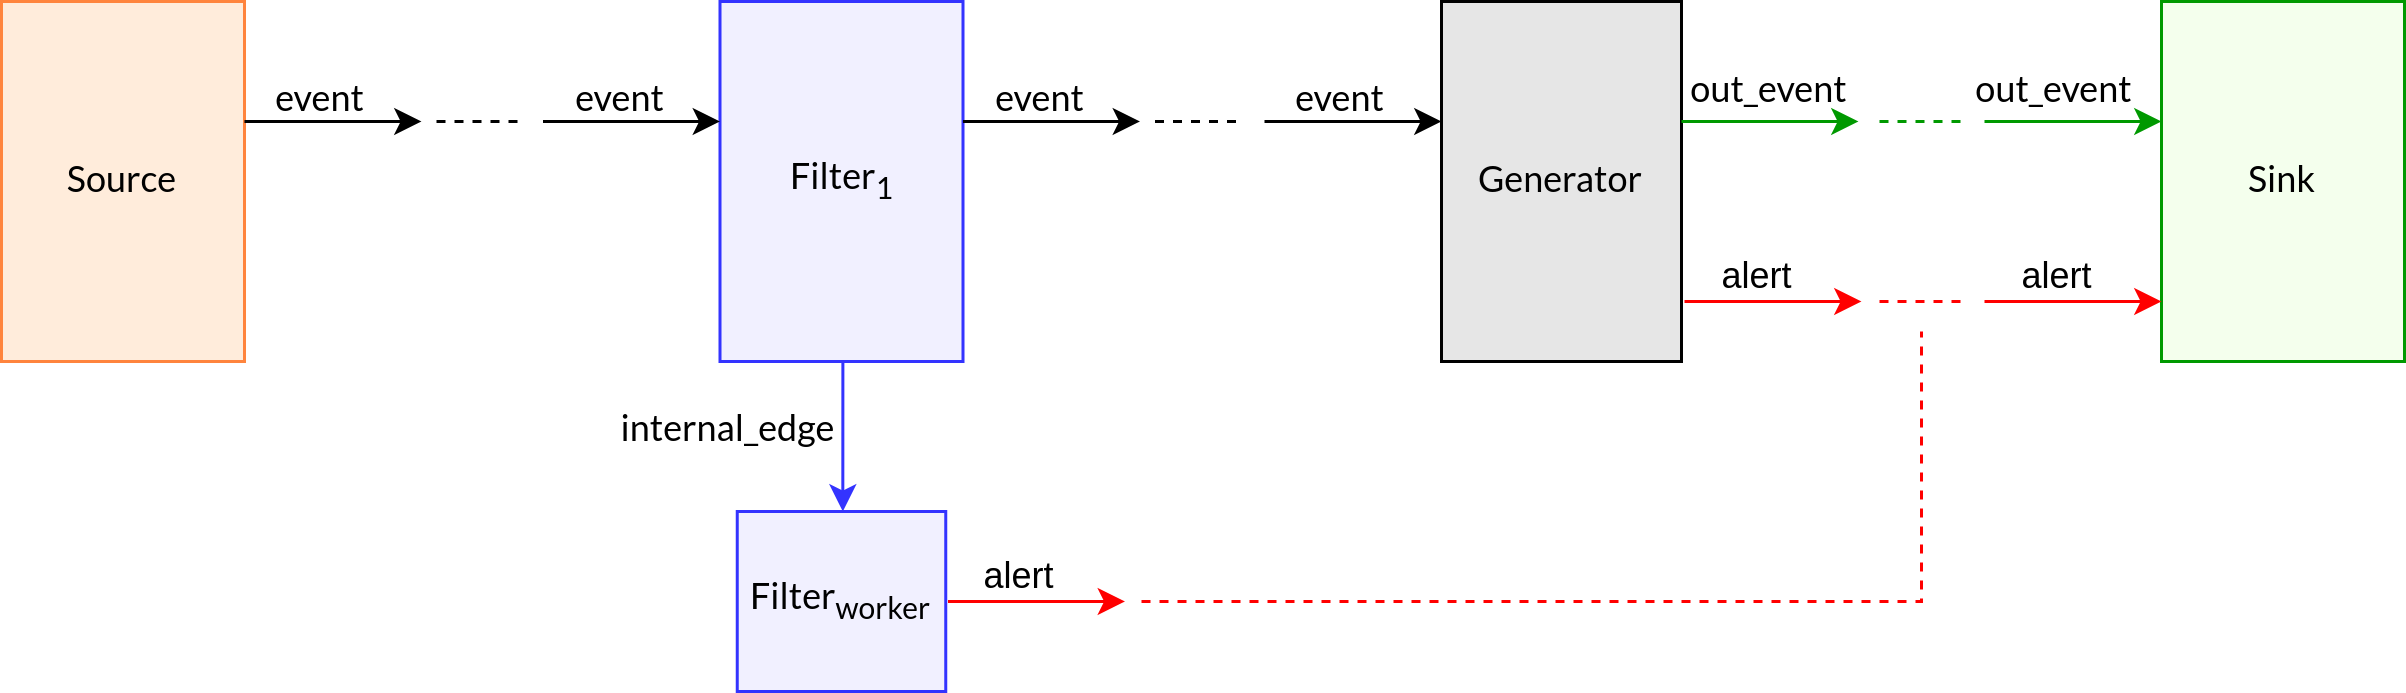
\includegraphics[scale = 0.7]{images/3-Engine/pipeline-schema-filter-detail-old.png}
  \caption{Pipeline Schema with Filter detail}
  \label{img:pipeline-schema-0}
\end{figure}

\begin{figure}[H]
  \centering
  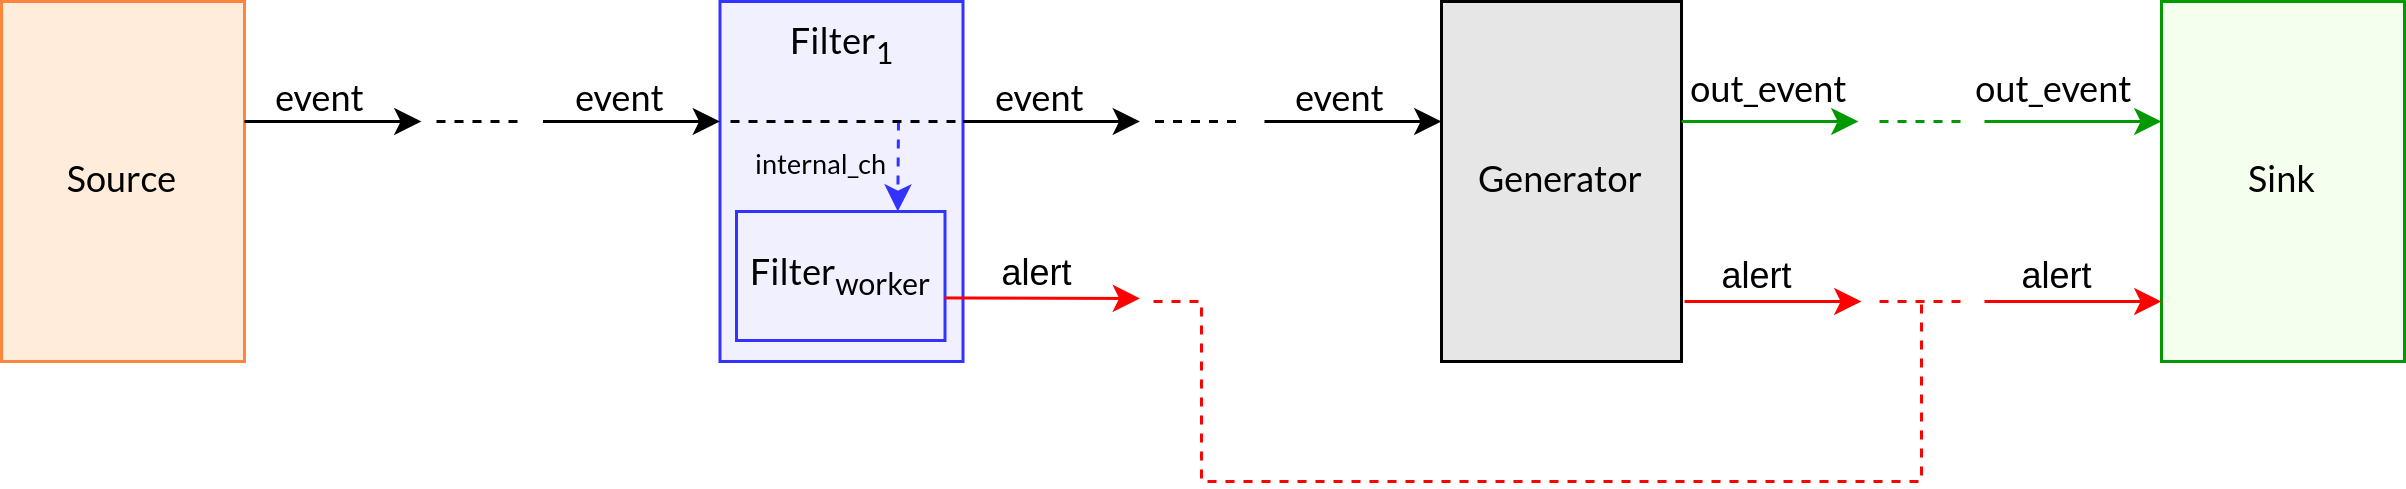
\includegraphics[scale = 0.7]{images/3-Engine/pipeline-schema-filter-detail-1.png}
  \caption{Pipeline Schema with Filter detail 1}
  \label{img:pipeline-schema-1}
\end{figure}

